% Options for packages loaded elsewhere
\PassOptionsToPackage{unicode}{hyperref}
\PassOptionsToPackage{hyphens}{url}
\PassOptionsToPackage{dvipsnames,svgnames*,x11names*}{xcolor}
%
\documentclass[
  12pt,
]{book}
\usepackage{lmodern}
\usepackage{amsmath}
\usepackage{ifxetex,ifluatex}
\ifnum 0\ifxetex 1\fi\ifluatex 1\fi=0 % if pdftex
  \usepackage[T1]{fontenc}
  \usepackage[utf8]{inputenc}
  \usepackage{textcomp} % provide euro and other symbols
  \usepackage{amssymb}
\else % if luatex or xetex
  \usepackage{unicode-math}
  \defaultfontfeatures{Scale=MatchLowercase}
  \defaultfontfeatures[\rmfamily]{Ligatures=TeX,Scale=1}
  \setmonofont[]{Source Code Pro}
\fi
% Use upquote if available, for straight quotes in verbatim environments
\IfFileExists{upquote.sty}{\usepackage{upquote}}{}
\IfFileExists{microtype.sty}{% use microtype if available
  \usepackage[]{microtype}
  \UseMicrotypeSet[protrusion]{basicmath} % disable protrusion for tt fonts
}{}
\makeatletter
\@ifundefined{KOMAClassName}{% if non-KOMA class
  \IfFileExists{parskip.sty}{%
    \usepackage{parskip}
  }{% else
    \setlength{\parindent}{0pt}
    \setlength{\parskip}{6pt plus 2pt minus 1pt}}
}{% if KOMA class
  \KOMAoptions{parskip=half}}
\makeatother
\usepackage{xcolor}
\IfFileExists{xurl.sty}{\usepackage{xurl}}{} % add URL line breaks if available
\IfFileExists{bookmark.sty}{\usepackage{bookmark}}{\usepackage{hyperref}}
\hypersetup{
  pdftitle={Notas Curso Básico R},
  pdfauthor={Tobías Chavarría},
  colorlinks=true,
  linkcolor=Maroon,
  filecolor=Maroon,
  citecolor=Blue,
  urlcolor=Blue,
  pdfcreator={LaTeX via pandoc}}
\urlstyle{same} % disable monospaced font for URLs
\usepackage{color}
\usepackage{fancyvrb}
\newcommand{\VerbBar}{|}
\newcommand{\VERB}{\Verb[commandchars=\\\{\}]}
\DefineVerbatimEnvironment{Highlighting}{Verbatim}{commandchars=\\\{\}}
% Add ',fontsize=\small' for more characters per line
\usepackage{framed}
\definecolor{shadecolor}{RGB}{248,248,248}
\newenvironment{Shaded}{\begin{snugshade}}{\end{snugshade}}
\newcommand{\AlertTok}[1]{\textcolor[rgb]{0.94,0.16,0.16}{#1}}
\newcommand{\AnnotationTok}[1]{\textcolor[rgb]{0.56,0.35,0.01}{\textbf{\textit{#1}}}}
\newcommand{\AttributeTok}[1]{\textcolor[rgb]{0.77,0.63,0.00}{#1}}
\newcommand{\BaseNTok}[1]{\textcolor[rgb]{0.00,0.00,0.81}{#1}}
\newcommand{\BuiltInTok}[1]{#1}
\newcommand{\CharTok}[1]{\textcolor[rgb]{0.31,0.60,0.02}{#1}}
\newcommand{\CommentTok}[1]{\textcolor[rgb]{0.56,0.35,0.01}{\textit{#1}}}
\newcommand{\CommentVarTok}[1]{\textcolor[rgb]{0.56,0.35,0.01}{\textbf{\textit{#1}}}}
\newcommand{\ConstantTok}[1]{\textcolor[rgb]{0.00,0.00,0.00}{#1}}
\newcommand{\ControlFlowTok}[1]{\textcolor[rgb]{0.13,0.29,0.53}{\textbf{#1}}}
\newcommand{\DataTypeTok}[1]{\textcolor[rgb]{0.13,0.29,0.53}{#1}}
\newcommand{\DecValTok}[1]{\textcolor[rgb]{0.00,0.00,0.81}{#1}}
\newcommand{\DocumentationTok}[1]{\textcolor[rgb]{0.56,0.35,0.01}{\textbf{\textit{#1}}}}
\newcommand{\ErrorTok}[1]{\textcolor[rgb]{0.64,0.00,0.00}{\textbf{#1}}}
\newcommand{\ExtensionTok}[1]{#1}
\newcommand{\FloatTok}[1]{\textcolor[rgb]{0.00,0.00,0.81}{#1}}
\newcommand{\FunctionTok}[1]{\textcolor[rgb]{0.00,0.00,0.00}{#1}}
\newcommand{\ImportTok}[1]{#1}
\newcommand{\InformationTok}[1]{\textcolor[rgb]{0.56,0.35,0.01}{\textbf{\textit{#1}}}}
\newcommand{\KeywordTok}[1]{\textcolor[rgb]{0.13,0.29,0.53}{\textbf{#1}}}
\newcommand{\NormalTok}[1]{#1}
\newcommand{\OperatorTok}[1]{\textcolor[rgb]{0.81,0.36,0.00}{\textbf{#1}}}
\newcommand{\OtherTok}[1]{\textcolor[rgb]{0.56,0.35,0.01}{#1}}
\newcommand{\PreprocessorTok}[1]{\textcolor[rgb]{0.56,0.35,0.01}{\textit{#1}}}
\newcommand{\RegionMarkerTok}[1]{#1}
\newcommand{\SpecialCharTok}[1]{\textcolor[rgb]{0.00,0.00,0.00}{#1}}
\newcommand{\SpecialStringTok}[1]{\textcolor[rgb]{0.31,0.60,0.02}{#1}}
\newcommand{\StringTok}[1]{\textcolor[rgb]{0.31,0.60,0.02}{#1}}
\newcommand{\VariableTok}[1]{\textcolor[rgb]{0.00,0.00,0.00}{#1}}
\newcommand{\VerbatimStringTok}[1]{\textcolor[rgb]{0.31,0.60,0.02}{#1}}
\newcommand{\WarningTok}[1]{\textcolor[rgb]{0.56,0.35,0.01}{\textbf{\textit{#1}}}}
\usepackage{longtable,booktabs}
\usepackage{calc} % for calculating minipage widths
% Correct order of tables after \paragraph or \subparagraph
\usepackage{etoolbox}
\makeatletter
\patchcmd\longtable{\par}{\if@noskipsec\mbox{}\fi\par}{}{}
\makeatother
% Allow footnotes in longtable head/foot
\IfFileExists{footnotehyper.sty}{\usepackage{footnotehyper}}{\usepackage{footnote}}
\makesavenoteenv{longtable}
\usepackage{graphicx}
\makeatletter
\def\maxwidth{\ifdim\Gin@nat@width>\linewidth\linewidth\else\Gin@nat@width\fi}
\def\maxheight{\ifdim\Gin@nat@height>\textheight\textheight\else\Gin@nat@height\fi}
\makeatother
% Scale images if necessary, so that they will not overflow the page
% margins by default, and it is still possible to overwrite the defaults
% using explicit options in \includegraphics[width, height, ...]{}
\setkeys{Gin}{width=\maxwidth,height=\maxheight,keepaspectratio}
% Set default figure placement to htbp
\makeatletter
\def\fps@figure{htbp}
\makeatother
\setlength{\emergencystretch}{3em} % prevent overfull lines
\providecommand{\tightlist}{%
  \setlength{\itemsep}{0pt}\setlength{\parskip}{0pt}}
\setcounter{secnumdepth}{5}
%\usepackage{inputenc}
% \usepackage{newpxtext,newpxmath}
\setcounter{tocdepth}{3}
\setcounter{secnumdepth}{3}
\usepackage[spanish]{babel}
\usepackage{booktabs}
\usepackage{csquotes}
\usepackage{amsmath, amsthm, amssymb,amsbsy}
\usepackage{mathtools}
\usepackage{graphics, graphicx}


% \usepackage{setspace}
% \doublespacing
%\addbibresource{bibliografia.bib}


% \usepackage{tcolorbox}
% \tcbuselibrary{theorems}
% \tcbuselibrary{breakable}
% 
% \newtcbtheorem[number within=section]{nota}{Nota}%
% {breakable, colback=yellow!5, colframe=yellow!40!gray,
% 	fonttitle=\bfseries}{nota}
% 
% \newtcbtheorem[number within=section,use counter
% from=nota]{cuidado}{Cuidado}%
% {breakable, colback=red!5, colframe=red!50!gray,
% 	fonttitle=\bfseries}{cuidado}
% 
% \newtcbtheorem[number within=section,use counter
% from=nota]{tarea}{Tarea}%
% {breakable, colback=blue!5, colframe=blue!35!black,
% 	fonttitle=\bfseries}{tarea}
% 
% \newtcbtheorem[number within=section,use counter
% from=nota]{solucion}{Solución}%
% {breakable, colback=gray!5, colframe=gray!35!black,
% 	fonttitle=\bfseries}{sol}
% 
% \newtcbtheorem[number within=section,use counter
% from=nota]{pregunta}{Pregunta}%
% {breakable,  colback=green!5, colframe=green!35!black,
% 	fonttitle=\bfseries}{preg}
% 
% \newtcbtheorem[number within=section,use counter
% from=nota]{ejemplo}{Ejemplo}%
% {breakable, colback=magenta!10, colframe=magenta!50!black,
% 	fonttitle=\bfseries}{ej}
% 
% \newtcbtheorem[number within=section,use counter
% from=nota]{laboratorio}{Laboratorio}%
% {breakable, colback=purple!10, colframe=purple!50!black,
% 	fonttitle=\bfseries}{lab}
%%end novalidate

%
%\usepackage{amsmath}
%\usepackage{amsthm}
%\usepackage{amssymb}
%%%% DEFINICIÓN DE ESTILOS DE TEOREMAS %%%
%\theoremstyle{definition}
%\newtheorem{definicion}{Definición}
%
%\theoremstyle{plain}
%\newtheorem{teorema}{Teorema}
%\newtheorem{lema}{Lema}
%%%%%%%%%%%%%%%%%%%%%%%%%%%%%%%%%%%%%%%%%%
\ifluatex
  \usepackage{selnolig}  % disable illegal ligatures
\fi

\title{Notas Curso Básico R}
\author{Tobías Chavarría}
\date{Actualizado el 01 Mar, 2021}

\begin{document}
\maketitle

{
\hypersetup{linkcolor=}
\setcounter{tocdepth}{4}
\tableofcontents
}
\hypertarget{introducciuxf3n}{%
\chapter{Introducción}\label{introducciuxf3n}}

Este documento contiene las bases del lenguaje de programación \textbf{R} para poder
empezar a realizar análisis de datos, se va a iniciar con la instalación y las
configuraciones básicas, y luego avanzaremos a los principios básicos del
lenguaje y las herramientas necesarias que nos permitan realizar un análisis
exploratorio de un conjunto de datos, construir funciones básicas y realizar visualizaciones.

\hypertarget{primeros-pasos-con-r-y-rstudio}{%
\chapter{\texorpdfstring{\textbf{Primeros pasos con R y RStudio}}{Primeros pasos con R y RStudio}}\label{primeros-pasos-con-r-y-rstudio}}

R es un entorno y lenguaje de programación con un enfoque al análisis estadístico

RStudio es un IDE por sus siglas en ingles Integrated Development Environment o Entorno De Desarrollo Integrado que facilita la interacción con el lenguaje de programación R y los procesos de carga de datos, instalación y administración de paquetes, exportación de gráficos y administración de archivos, entre otros.

El objetivo de este capítulo es conocer el entorno de trabajo que proporciona R y RStudio, además de aprender a instalar y cargar los paquetes que se necesiten para realizar análisis de datos.

\hypertarget{instalaciuxf3n}{%
\section{\texorpdfstring{\textbf{Instalación}}{Instalación}}\label{instalaciuxf3n}}

\hypertarget{r}{%
\subsection{\texorpdfstring{\textbf{R}}{R}}\label{r}}

Para instalar R en Windows, la forma más simple es descargar la versión más reciente de R base desde el siguiente enlace de CRAN:

\url{https://cran.r-project.org/bin/windows/base/}

El archivo que necesitamos tiene la extensión \textbf{.exe} (por ejemplo 4.0.2-win.exe). Una vez descargado, lo ejecutamos como cualquier instalable.

Después de la instalación, estamos listos para usar R.

\hypertarget{rstudio}{%
\subsection{\texorpdfstring{\textbf{RStudio}}{RStudio}}\label{rstudio}}

Para instalar RStudio, es necesario descargar y ejecutar alguno de los instaladores disponibles en su sitio oficial. Están disponibles versiones para Windows, OSX y Linux.

\url{https://www.rstudio.com/products/rstudio/download/}

Si ya hemos instalado R en nuestro equipo, RStudio lo detectará automáticamente y podremos utilizarlo desde este entorno. Si no instalamos RStudio antes que R, no hay problema, cada vez que iniciamos este programa, verificará la instalación de R.

\hypertarget{entorno-de-trabajo-de-rstudio.}{%
\section{\texorpdfstring{\textbf{Entorno de trabajo de RStudio.}}{Entorno de trabajo de RStudio.}}\label{entorno-de-trabajo-de-rstudio.}}

En general se trabaja con la interfaz de RStudio antes que con la de R porque la primera es mucho ``más amigable.''

Al abrir RStudio veremos algo como esto:

\begin{center}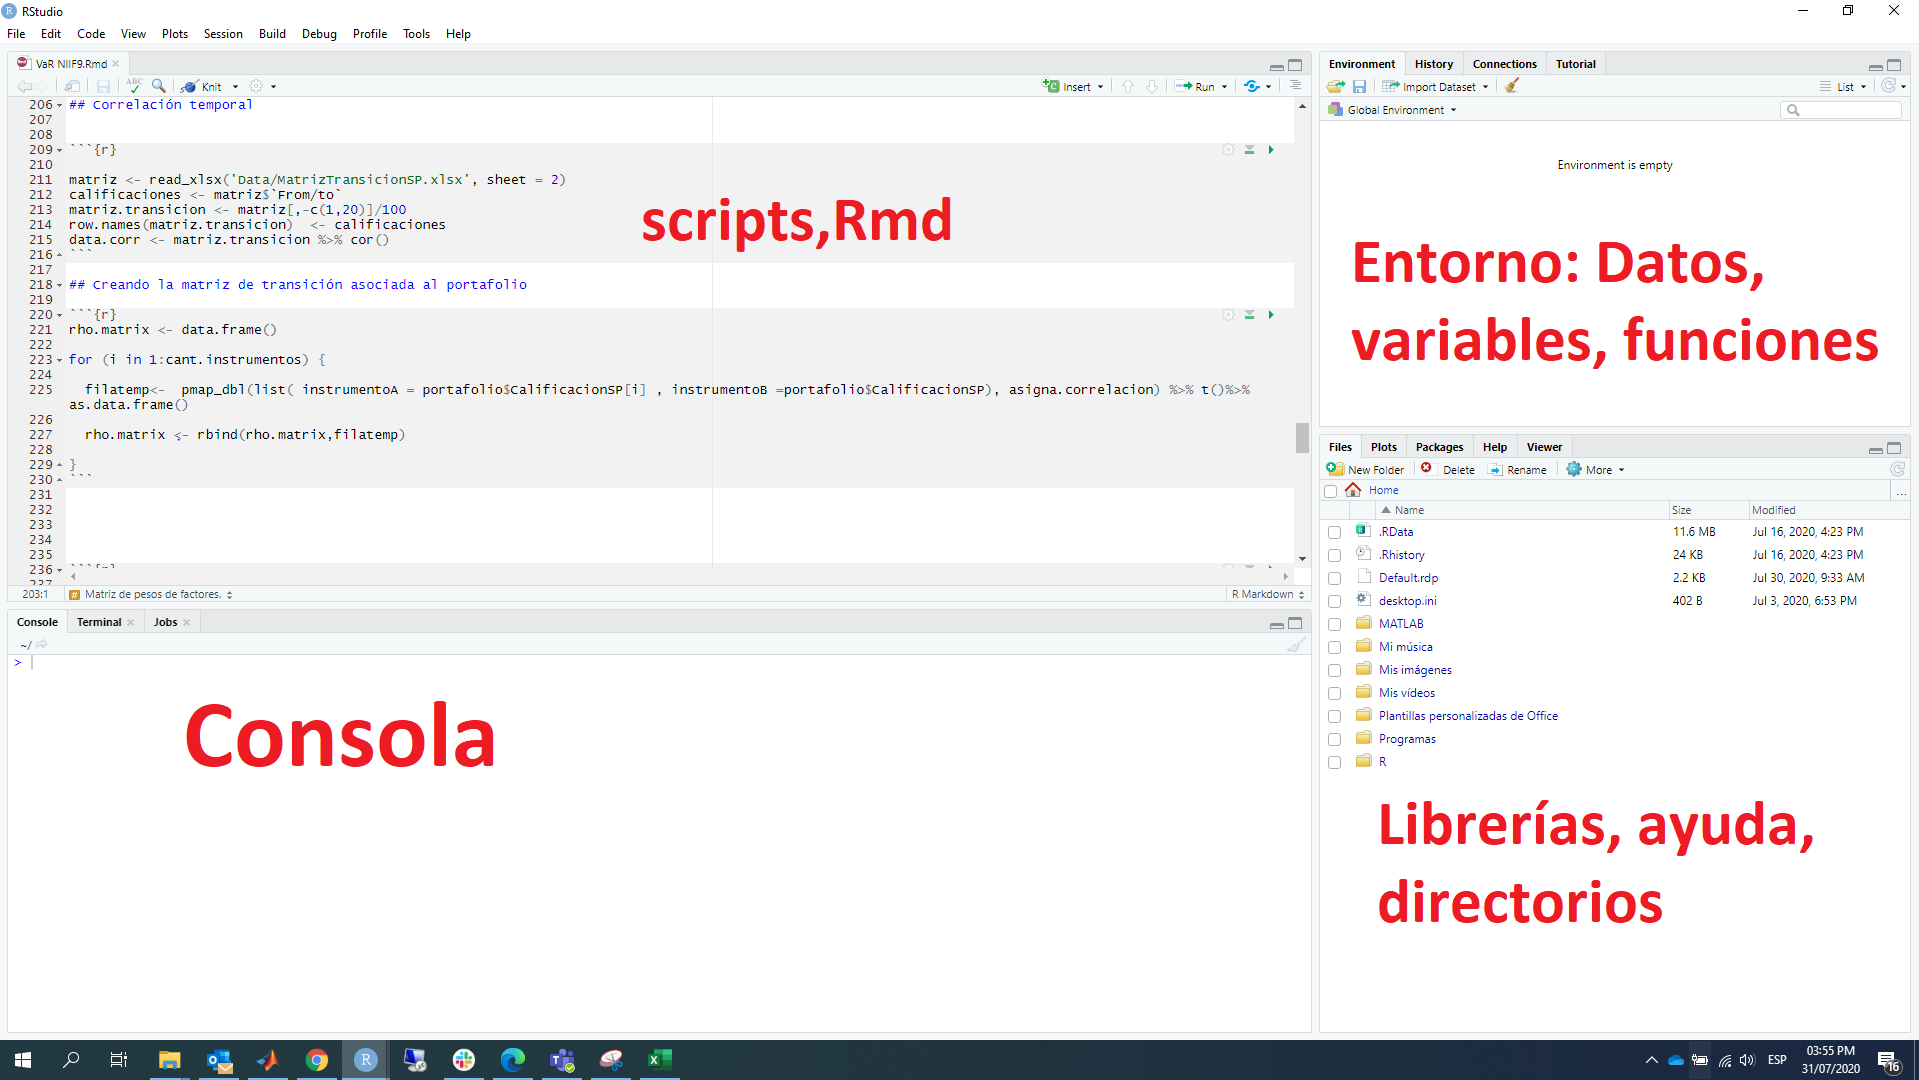
\includegraphics[width=1\linewidth]{images/entornoRStudio} \end{center}

Una vez estamos en RStudio, podemos escribir y ejecutar las órdenes de varias formas:

\begin{itemize}
\tightlist
\item
  Directamente en la consola
\item
  A través de un script (.R)
\item
  Con ficheros Rmarkdown (.Rmd)
\end{itemize}

\hypertarget{consola-de-r}{%
\subsection{\texorpdfstring{\textbf{Consola de R}}{Consola de R}}\label{consola-de-r}}

La consola de RStudio nos permite interactuar con los comandos de R, es decir, ingresamos una instrucción en la consola y esta retornará el resultado de la ejecución de ese comando, aunque esta es una herramienta muy útil no es la mejor opción cuando nuestro código gana complejidad.

En la consola escribimos \textbf{expresiones}, el símbolo ``\textless-'' es el operador de asignación, aunque también se puede utilizar el símbolo ``=.''

\textbf{Asignación de valores.}

\begin{Shaded}
\begin{Highlighting}[]
\NormalTok{x }\OtherTok{\textless{}{-}} \DecValTok{1}  \CommentTok{\# Asignamos el valor 1 a la variable x}

\NormalTok{texto }\OtherTok{\textless{}{-}} \StringTok{"Bienvenidos"}  \CommentTok{\# Asignamos el valor "Bienvenidos" a la variable texto}
\end{Highlighting}
\end{Shaded}

En R el símbolo ``\#'' indica que es un comentario, cualquier cosa que esté a su derecha (incluido el ``\#'') será ignorado a la hora de ejecutar el código. Este es el único símbolo para hacer comentarios en R y además cabe mencionar que R no soporta comentarios en bloques o multilíneas.

\textbf{Evaluación.}

Cuando escribimos una expresión en la consola, podemos imprimir su valor sin una orden explícita.

\begin{Shaded}
\begin{Highlighting}[]
\NormalTok{x }\OtherTok{\textless{}{-}} \DecValTok{13} \CommentTok{\# No imprime nada, solo asigna el valor}
\end{Highlighting}
\end{Shaded}

\begin{Shaded}
\begin{Highlighting}[]
\NormalTok{x }\CommentTok{\# Se imprime el valor}
\end{Highlighting}
\end{Shaded}

\begin{verbatim}
## [1] 13
\end{verbatim}

\begin{Shaded}
\begin{Highlighting}[]
\FunctionTok{print}\NormalTok{(x) }\CommentTok{\# Orden explicita}
\end{Highlighting}
\end{Shaded}

\begin{verbatim}
## [1] 13
\end{verbatim}

\hypertarget{ayuda-en-r}{%
\subsection{\texorpdfstring{\textbf{Ayuda en R}}{Ayuda en R}}\label{ayuda-en-r}}

Al comenzar a trabajar con R necesitaremos información sobre cada instrucción,
función y paquete. Toda la documentación se encuentra integrada en RStudio, para accesar a esta información podemos usar la función \textbf{help()} o el signo de interrogación \textbf{?}, de la siguiente manera

\begin{Shaded}
\begin{Highlighting}[]
\FunctionTok{help}\NormalTok{(}\StringTok{"funcion"}\NormalTok{)}

\NormalTok{?funcion}
\NormalTok{??nombre\_paquete}
\end{Highlighting}
\end{Shaded}

Al ejecutar estas instrucciones la información aparece en la pestaña de \textbf{help}.

\begin{Shaded}
\begin{Highlighting}[]
\FunctionTok{help}\NormalTok{(}\StringTok{"read.table"}\NormalTok{)}

\NormalTok{?read.table}
\end{Highlighting}
\end{Shaded}

\hypertarget{nombres-en-r}{%
\subsection{\texorpdfstring{\textbf{Nombres en R}}{Nombres en R}}\label{nombres-en-r}}

Al igual que la documentación de nuestro código, es importante el nombre que le demos a nuestros objetos (variables, funciones). En \textbf{R} los nombres de los objetos deben comenzar con una letra y solo pueden contener letras, números y los signos : "\emph{" , ``.'' Es bueno que los nombres sean descriptivos, es necesario adoptar una convención, la más común es la del guión bajo (snake\_case) en la que los nombres se escriben en minúscula y separados por } .

\begin{Shaded}
\begin{Highlighting}[]
\NormalTok{yo\_uso\_guion\_bajo  }\DocumentationTok{\#\# snake\_case}

\NormalTok{OtraGenteUsaMayusculas}

\NormalTok{algunas.personas.usan.puntos }\DocumentationTok{\#\# Esto es peculiar de R, ya que en otros lenguajes el punto no se acepta en los nombres}
\DocumentationTok{\#\# ya que tiene otras funciones}

\NormalTok{Y\_algunasPocas.Personas\_RENIEGANdelasconvenciones}
\end{Highlighting}
\end{Shaded}

Generalmente las variables son sustantivos y el nombre de las funciones verbos, se debe procurar que los nombres sean concisos y con significado.

\begin{Shaded}
\begin{Highlighting}[]
\DocumentationTok{\#\# Correcto}

\NormalTok{dia\_uno }\OtherTok{\textless{}{-}} \DecValTok{10}

\DocumentationTok{\#\# Incorrecto}

\NormalTok{primer\_dia\_del\_mes }\OtherTok{\textless{}{-}} \DecValTok{10}
\end{Highlighting}
\end{Shaded}

También se debe evitar utilizar nombres de funciones o variables comunes, esto causa confusión al leer el código.

\begin{Shaded}
\begin{Highlighting}[]
\DocumentationTok{\#\# Incorrecto}

\NormalTok{T }\OtherTok{\textless{}{-}} \ConstantTok{FALSE}
\NormalTok{c }\OtherTok{\textless{}{-}} \DecValTok{10}

\NormalTok{mean }\OtherTok{\textless{}{-}} \ControlFlowTok{function}\NormalTok{(x) \{}
  \FunctionTok{sum}\NormalTok{(x)}
\NormalTok{\}}
\end{Highlighting}
\end{Shaded}

Existen muchas otras buenas prácticas a la hora de escribir código en \textbf{R}, el siguiente link contiene una guía del estilo \emph{tidyverse}.

\url{https://style.tidyverse.org/index.html}

\hypertarget{scripts-de-r}{%
\subsection{\texorpdfstring{\textbf{Scripts de R}}{Scripts de R}}\label{scripts-de-r}}

Trabajar en la consola es muy limitado ya que las instrucciones se tienen que escribir una por una. Lo habitual es trabajar con scripts o ficheros de instrucciones. Estos ficheros tienen extensión \textbf{.R}.

Se puede crear una script con cualquier editor de texto, pero nosotros lo haremos desde RStudio. Para hacer esto, seleccionamos la siguiente ruta de menús: File \textgreater{} New File \textgreater{} R script

\begin{center}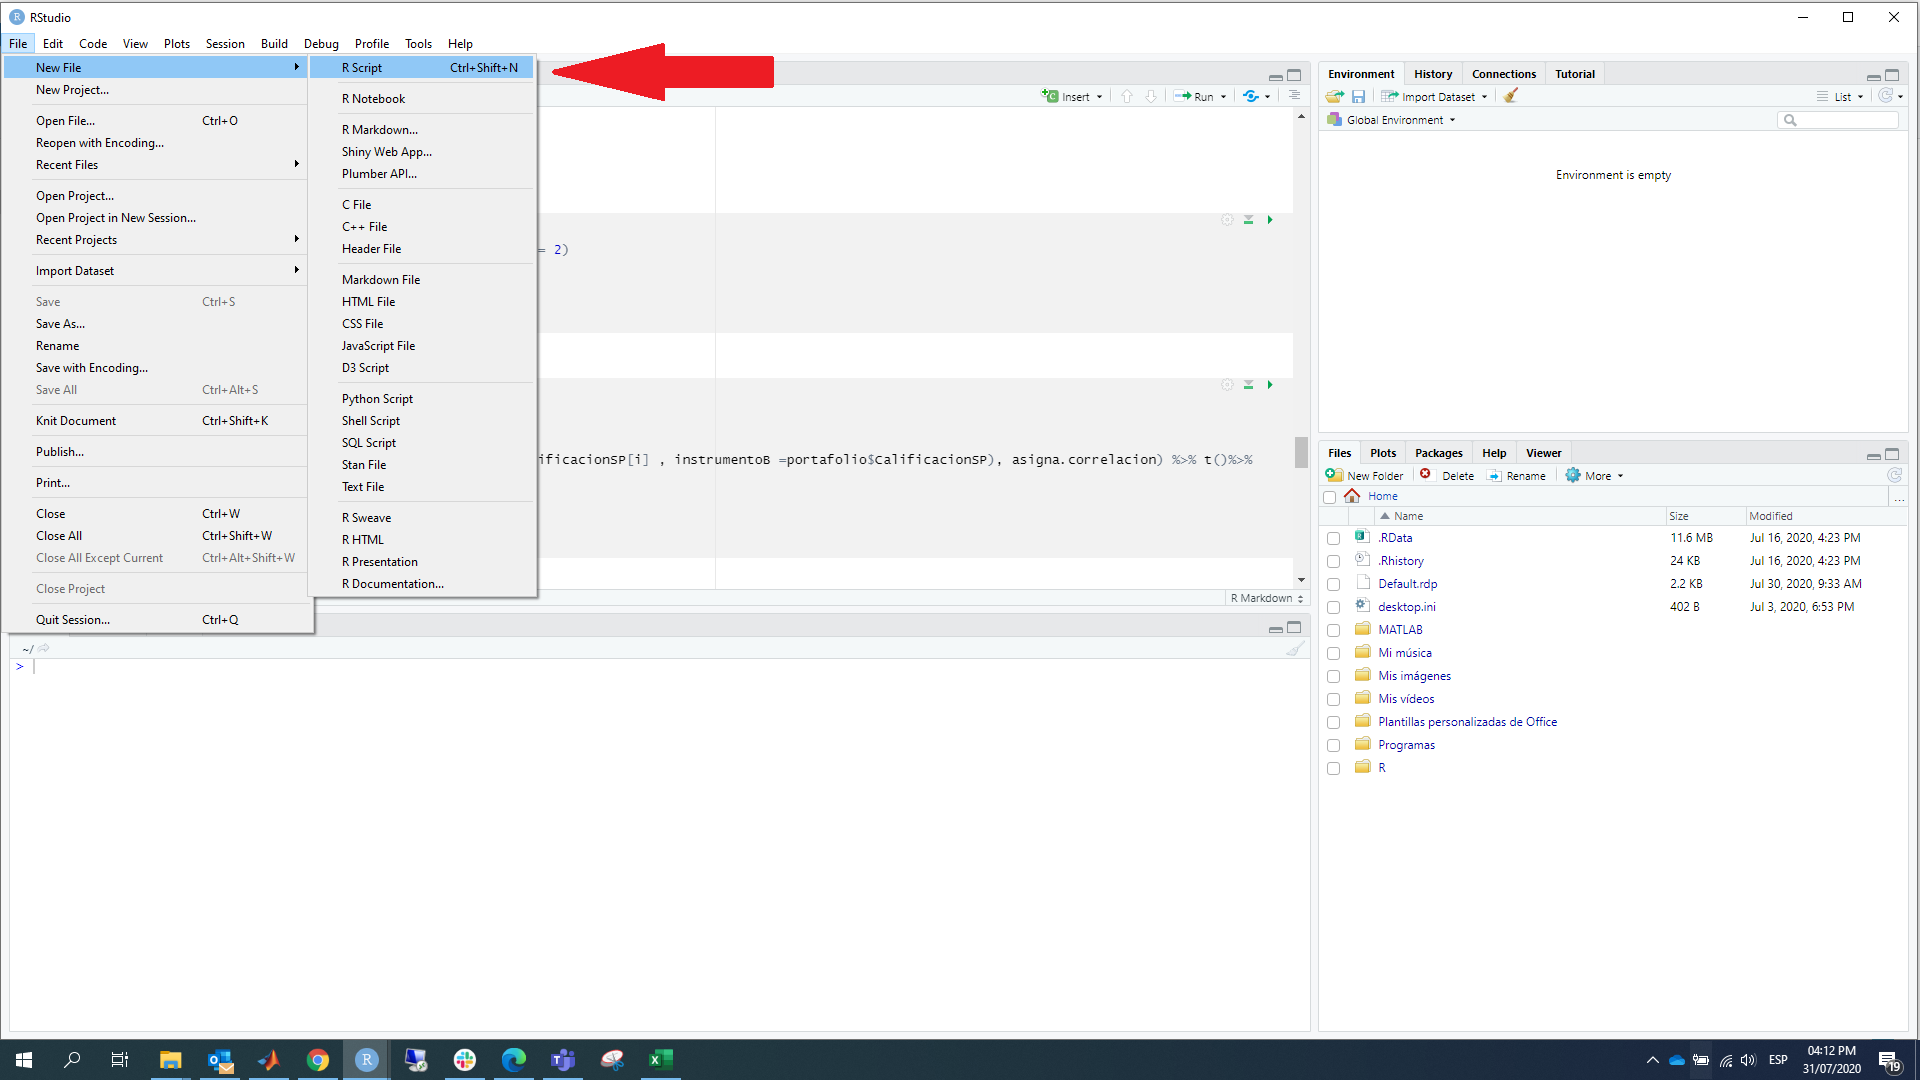
\includegraphics[width=1\linewidth]{images/script} \end{center}

\hypertarget{entorno}{%
\subsection{\texorpdfstring{\textbf{Entorno}}{Entorno}}\label{entorno}}

El panel de entorno esta compuesto de dos pestañas: Environment y History.

En el entorno se irán registrando los objetos que vayamos creando en la sesión de trabajo: datos, variables, funciones. También tenemos la opción de cargar y guardar una sesión de trabajo, importar datos y limpiar los objetos de la sesión. Estas opciones están accesibles a través de las de opciones de la pestaña.

\begin{center}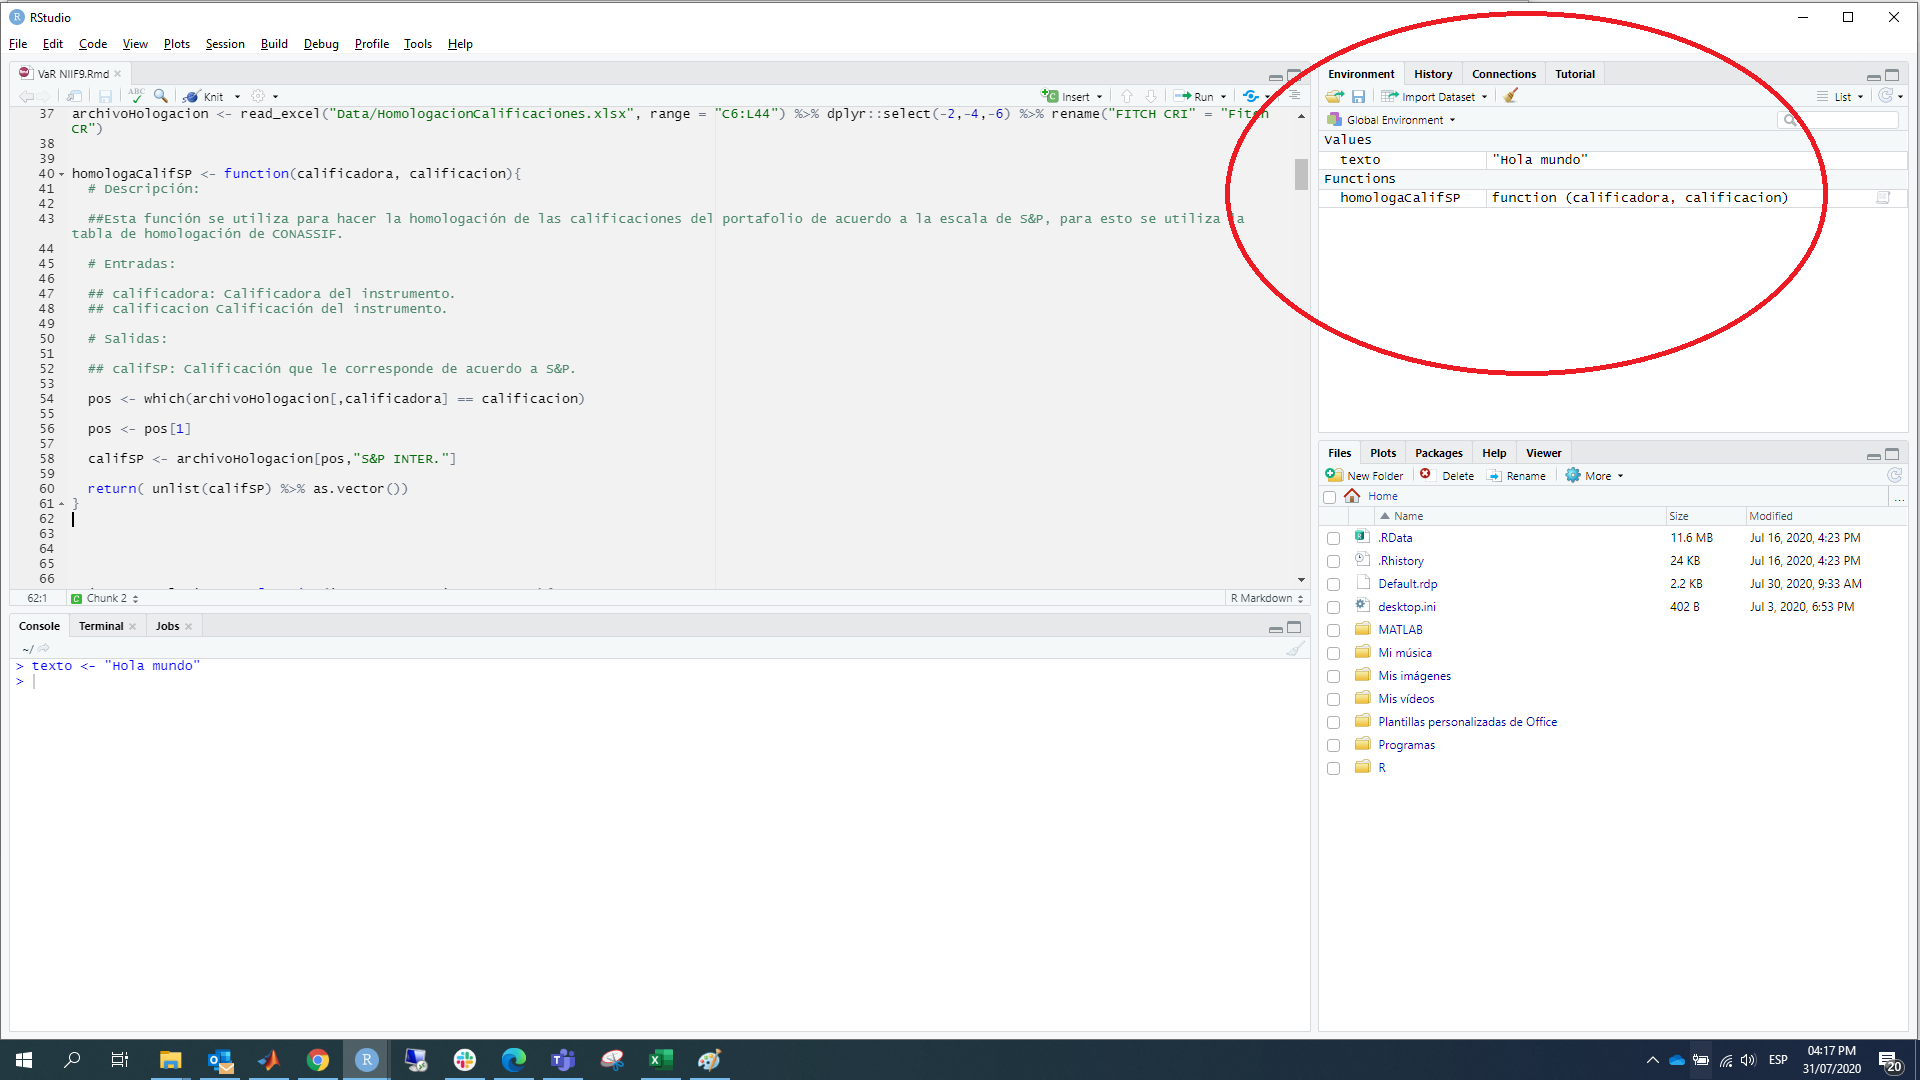
\includegraphics[width=1\linewidth]{images/entorno} \end{center}

\hypertarget{directorio-de-trabajo}{%
\subsection{\texorpdfstring{\textbf{Directorio de trabajo}}{Directorio de trabajo}}\label{directorio-de-trabajo}}

El directorio o carpeta de trabajo es el lugar en la computadora en el que se encuentran los archivos con los que se van a trabajar en R. Este es el lugar donde R buscara archivos para importarlos y al que serán exportados, a menos que indiquemos otra cosa.

Para encontrar cuál es el directorio de trabajo actual se utiliza la función \textbf{getwd()}.

\begin{Shaded}
\begin{Highlighting}[]
\FunctionTok{getwd}\NormalTok{()}
\end{Highlighting}
\end{Shaded}

\begin{verbatim}
## [1] "/Users/tchavarria/Documents/GitHub/programacion-r-basico"
\end{verbatim}

Se mostrará en la consola la ruta del directorio que está usando R.

Se puede cambiar el directorio de trabajo usando la función setwd(), dando como argumento la ruta del directorio que se desea utilizar.

\begin{Shaded}
\begin{Highlighting}[]
\FunctionTok{setwd}\NormalTok{(}\StringTok{"otra\_ruta"}\NormalTok{)}
\end{Highlighting}
\end{Shaded}

\hypertarget{paquetes}{%
\section{\texorpdfstring{\textbf{Paquetes}}{Paquetes}}\label{paquetes}}

Cada paquete es una colección de funciones diseñadas para atender una tarea específica. Por ejemplo, hay paquetes para trabajo visualización, conexiones a bases de datos, minería de datos, interacción con servicios de internet, entre otros.

Estos paquetes se encuentran alojados en CRAN, así que pasan por un control riguroso antes de estar disponibles para su uso generalizado.

Se pueden instalar paquetes usando la función \textbf{install.packages()}, dando como argumento el nombre del paquete que deseamos instalar, entre comillas.

Por ejemplo, para instalar el paquete \textbf{dplyr}, ejecutamos lo siguiente.

\begin{Shaded}
\begin{Highlighting}[]
\FunctionTok{install.packages}\NormalTok{(}\StringTok{"dplyr"}\NormalTok{) }\DocumentationTok{\#\# En general se escribe  install.packages("nombre\_paquete")}
\end{Highlighting}
\end{Shaded}

Después de ejecutar esa instrucción, aparecerán algunos mensajes en la consola mostrando el avance de la instalación

Una vez concluida la instalación de un paquete, para poder utilizar sus funciones debemos ejecutar la función \textbf{library()} con el nombre del paquete que se quiere utilizar.

\begin{Shaded}
\begin{Highlighting}[]
\FunctionTok{library}\NormalTok{(dplyr)   }\DocumentationTok{\#\# En general se escribe  library("nombre\_paquete")}
\end{Highlighting}
\end{Shaded}

\hypertarget{scripts}{%
\section{\texorpdfstring{\textbf{Scripts}}{Scripts}}\label{scripts}}

Los scripts son documentos de texto con la extensión de archivo .R, por ejemplo mi\_script.R.

Estos archivos son iguales a cualquier documentos de texto, pero R los puede leer y ejecutar el código que contienen.

Aunque R permite el uso interactivo, es recomendable guardar el código en un archivo .R, de esta manera se puede utilizar después y compartirlo con otras personas. En general, en proyectos complejos, es posible que sean necesarios múltiples scripts para distintos fines.

Se pueden abrir y ejecutar scripts en R usando la función \textbf{source()}, esta recibe como argumento la ruta del archivo .R en nuestra computadora, entre comillas.

Por ejemplo.

\begin{Shaded}
\begin{Highlighting}[]
\FunctionTok{source}\NormalTok{(}\StringTok{"C:/Proyecto/limpiezaDatos.R"}\NormalTok{)}
\end{Highlighting}
\end{Shaded}

Cuando usamos RStudio y abrimos un script con extensión .R, este programa abre un panel en el que se puede ver su contenido. De este modo se puede ejecutar todo el código que contiene o sólo partes de él.

\hypertarget{shortcuts}{%
\section{\texorpdfstring{\textbf{Shortcuts}}{Shortcuts}}\label{shortcuts}}

\begin{itemize}
\tightlist
\item
  Borrar toda la consola: CTRL + L.
\item
  Ejecutar una línea o lo que se seleccione: CTRL+R
\end{itemize}

\hypertarget{objetos-en-r.}{%
\chapter{\texorpdfstring{\textbf{Objetos en R.}}{Objetos en R.}}\label{objetos-en-r.}}

En R tenemos 5 clases de objeto básicos o atómicos:

\begin{itemize}
\tightlist
\item
  character
\item
  numeric
\item
  integer
\item
  complex
\item
  logical (TRUE/FALSE)
\end{itemize}

\begin{Shaded}
\begin{Highlighting}[]
\NormalTok{tipo.bien }\OtherTok{\textless{}{-}} \StringTok{"Vivienda"}   \DocumentationTok{\#\# character}

\NormalTok{saldo }\OtherTok{\textless{}{-}} \FloatTok{130500.34}        \DocumentationTok{\#\# numeric}

\NormalTok{meses }\OtherTok{\textless{}{-}} \DecValTok{13}               \DocumentationTok{\#\# numeric}

\NormalTok{dias.mora }\OtherTok{\textless{}{-}}\NormalTok{ 10L          }\DocumentationTok{\#\# integer}

\NormalTok{complejo }\OtherTok{\textless{}{-}} \DecValTok{1} \SpecialCharTok{+}\NormalTok{ 3i         }\DocumentationTok{\#\# complex}

\NormalTok{cobro.judicial }\OtherTok{\textless{}{-}} \ConstantTok{TRUE}    \DocumentationTok{\#\# logical}
\end{Highlighting}
\end{Shaded}

\textbf{Números.}

\begin{itemize}
\tightlist
\item
  En R los número en general se tratan como objetos numeric (i.e números reales de doble precisión.)
\item
  Existe el valor \textbf{Inf} que representa infinito y se asocia a operaciones como : 1/0.
\end{itemize}

\begin{Shaded}
\begin{Highlighting}[]
\DecValTok{1} \SpecialCharTok{/} \DecValTok{0}
\end{Highlighting}
\end{Shaded}

\begin{verbatim}
## [1] Inf
\end{verbatim}

\begin{Shaded}
\begin{Highlighting}[]
\SpecialCharTok{{-}}\DecValTok{1} \SpecialCharTok{/} \DecValTok{0}
\end{Highlighting}
\end{Shaded}

\begin{verbatim}
## [1] -Inf
\end{verbatim}

\begin{Shaded}
\begin{Highlighting}[]
\DecValTok{100} \SpecialCharTok{/} \ConstantTok{Inf}
\end{Highlighting}
\end{Shaded}

\begin{verbatim}
## [1] 0
\end{verbatim}

\begin{itemize}
\tightlist
\item
  El valor \textbf{NaN} significa not a number, este se asocia generalmente a datos ausentes pero también a una operación del tipo 0/0 que no está definida.
\end{itemize}

\textbf{Atributos}

Los objetos en R pueden tener los siguientes atributos

\begin{itemize}
\tightlist
\item
  names, dimnames (matrices, data frames)
\item
  dimension (matrices, data frames)
\item
  class
\item
  length
\end{itemize}

más adelante veremos que con detalle el uso de estos.

\hypertarget{operadores}{%
\chapter{\texorpdfstring{\textbf{Operadores}}{Operadores}}\label{operadores}}

\textbf{Operadores aritméticos}

En R tenemos los siguientes operadores aritméticos:

\begin{longtable}[]{@{}rrlll@{}}
\toprule
Operador & Operación & Ejemplo & Resultado &\tabularnewline
\midrule
\endhead
+ & Suma & 3+1 & 4 &\tabularnewline
- & Resta & 4-6 & -2 &\tabularnewline
* & Multiplicación & 4*6 & 24 &\tabularnewline
/ & División & 14/5 & 2.8 &\tabularnewline
\^{} & Potencia & 2\^{}3 & 8 &\tabularnewline
\%\% & División entera & 5\%\%2 & 1 &\tabularnewline
\bottomrule
\end{longtable}

\textbf{Operadores relacionales}

Los operadores relacionales son usados para hacer comparaciones y siempre devuelven como resultado TRUE o FALSE (verdadero o falso, respectivamente).

\begin{longtable}[]{@{}rrlll@{}}
\toprule
Operador & Operación & Ejemplo & Resultado &\tabularnewline
\midrule
\endhead
\textless{} & Menor estricto & 10 \textless{} 3 & FALSE &\tabularnewline
\textless= & Menor o igual & 10 \textless= 3 & FALSE &\tabularnewline
\textgreater{} & Mayor estricto & 10 \textgreater{} 3 & TRUE &\tabularnewline
\textgreater= & Mayor o igual & 10 \textgreater= 3 & TRUE &\tabularnewline
== & Igual & 10 == 3 & FALSE &\tabularnewline
!= & Distinto & 10 != 3 & TRUE &\tabularnewline
\bottomrule
\end{longtable}

\textbf{Operadores lógicos}

Los operadores lógicos son usados para operaciones de álgebra Booleana, es decir, para describir relaciones lógicas, expresadas como verdadero (TRUE) o falso (FALSO).

\begin{longtable}[]{@{}rrl@{}}
\toprule
Operador & Operación &\tabularnewline
\midrule
\endhead
\textbar{} & or &\tabularnewline
\& & and (conjunción) &\tabularnewline
! & negación &\tabularnewline
\bottomrule
\end{longtable}

Los operadores \textbar{} y \& siguen estas reglas:

\begin{itemize}
\tightlist
\item
  \textbar{} devuelve TRUE si alguno de los datos es TRUE
\item
  \& solo devuelve TRUE si ambos datos es TRUE
\item
  \textbar{} solo devuelve FALSE si ambos datos son FALSE
\item
  \& devuelve FALSE si alguno de los datos es FALSE
\end{itemize}

\begin{Shaded}
\begin{Highlighting}[]
\NormalTok{edad }\OtherTok{\textless{}{-}} \DecValTok{16}
\NormalTok{notas }\OtherTok{\textless{}{-}} \DecValTok{83}

\NormalTok{beca1 }\OtherTok{\textless{}{-}}\NormalTok{ (edad }\SpecialCharTok{\textgreater{}} \DecValTok{18} \SpecialCharTok{\&}\NormalTok{ notas }\SpecialCharTok{\textgreater{}} \DecValTok{80}\NormalTok{)}

\NormalTok{beca1}
\end{Highlighting}
\end{Shaded}

\begin{verbatim}
## [1] FALSE
\end{verbatim}

\begin{Shaded}
\begin{Highlighting}[]
\NormalTok{beca2 }\OtherTok{\textless{}{-}}\NormalTok{ (edad }\SpecialCharTok{\textgreater{}} \DecValTok{18} \SpecialCharTok{|}\NormalTok{ notas }\SpecialCharTok{\textgreater{}} \DecValTok{80}\NormalTok{)}

\NormalTok{beca2}
\end{Highlighting}
\end{Shaded}

\begin{verbatim}
## [1] TRUE
\end{verbatim}

\hypertarget{estructuras-de-datos.}{%
\chapter{\texorpdfstring{\textbf{Estructuras de datos.}}{Estructuras de datos.}}\label{estructuras-de-datos.}}

Las estructuras de datos básicas de R se pueden agrupar por su dimensionalidad y según si son homogéneas (todos los elementos son del mismo tipo) o heterogéneas (hay elementos de distintos tipos). En el siguiente cuadro se resumen estas:

\begin{longtable}[]{@{}rrl@{}}
\toprule
Dimensión & Homogéneas & Heterogéneas\tabularnewline
\midrule
\endhead
1d & Vector & Lista\tabularnewline
2d & Matriz & Data Frame\tabularnewline
\bottomrule
\end{longtable}

\hypertarget{vectores}{%
\section{\texorpdfstring{\textbf{Vectores}}{Vectores}}\label{vectores}}

Los vectores en R son fundamentales ya que, es una de las estructuras de datos más utilizada, la propiedad más importante de los vectores, es que \textbf{solo pueden contener objetos de la misma clase}.

Vectores vacíos pueden crearse con la función \textbf{vector()}, por ejemplo:

\begin{Shaded}
\begin{Highlighting}[]
\FunctionTok{vector}\NormalTok{(}\StringTok{"numeric"}\NormalTok{, }\AttributeTok{length =} \DecValTok{10}\NormalTok{) }\DocumentationTok{\#\# Tiene los parámetros clase y longitud.}
\end{Highlighting}
\end{Shaded}

\begin{verbatim}
##  [1] 0 0 0 0 0 0 0 0 0 0
\end{verbatim}

\begin{Shaded}
\begin{Highlighting}[]
\FunctionTok{vector}\NormalTok{(}\StringTok{"character"}\NormalTok{, }\DecValTok{3}\NormalTok{)}
\end{Highlighting}
\end{Shaded}

\begin{verbatim}
## [1] "" "" ""
\end{verbatim}

Sin embargo, la forma más común para crear vectores es utilizando la función \textbf{c()} que hace referencia a la palabra concatenar.

\begin{Shaded}
\begin{Highlighting}[]
\NormalTok{vector.numerico }\OtherTok{\textless{}{-}} \FunctionTok{c}\NormalTok{(}\DecValTok{1}\NormalTok{, }\DecValTok{2}\NormalTok{, }\FloatTok{3.5}\NormalTok{)   }\DocumentationTok{\#\# numeric}

\NormalTok{vector.logical }\OtherTok{\textless{}{-}} \FunctionTok{c}\NormalTok{(}\ConstantTok{TRUE}\NormalTok{, }\ConstantTok{FALSE}\NormalTok{, T, T, F) }\DocumentationTok{\#\# logical}

\NormalTok{vector.char }\OtherTok{\textless{}{-}} \FunctionTok{c}\NormalTok{(}\StringTok{"Azul"}\NormalTok{, }\StringTok{"Blanco"}\NormalTok{, }\StringTok{"Verde"}\NormalTok{) }\DocumentationTok{\#\# character}

\NormalTok{vector.entero }\OtherTok{\textless{}{-}} \DecValTok{1}\SpecialCharTok{:}\DecValTok{13}   \DocumentationTok{\#\# integer}
\end{Highlighting}
\end{Shaded}

\begin{Shaded}
\begin{Highlighting}[]
\NormalTok{vector.numerico}
\end{Highlighting}
\end{Shaded}

\begin{verbatim}
## [1] 1.0 2.0 3.5
\end{verbatim}

\begin{Shaded}
\begin{Highlighting}[]
\NormalTok{vector.logical}
\end{Highlighting}
\end{Shaded}

\begin{verbatim}
## [1]  TRUE FALSE  TRUE  TRUE FALSE
\end{verbatim}

\begin{Shaded}
\begin{Highlighting}[]
\NormalTok{vector.char}
\end{Highlighting}
\end{Shaded}

\begin{verbatim}
## [1] "Azul"   "Blanco" "Verde"
\end{verbatim}

\begin{Shaded}
\begin{Highlighting}[]
\NormalTok{vector.entero}
\end{Highlighting}
\end{Shaded}

\begin{verbatim}
##  [1]  1  2  3  4  5  6  7  8  9 10 11 12 13
\end{verbatim}

\hypertarget{coerciuxf3n}{%
\subsection{\texorpdfstring{\textbf{Coerción}}{Coerción}}\label{coerciuxf3n}}

Como dijimos anteriormente los vectores solo contienen una misma clase de datos, sin embargo, cuando mezclamos diferentes clases ocurre automáticamente un proceso que se llama \textbf{coerción}, esto básicamente transforma todos los elementos del vector a una misma clase.

\begin{Shaded}
\begin{Highlighting}[]
\NormalTok{vector.prueba1 }\OtherTok{\textless{}{-}} \FunctionTok{c}\NormalTok{(}\FloatTok{1.3}\NormalTok{, }\StringTok{"Diego"}\NormalTok{) }\CommentTok{\# character}
\NormalTok{vector.prueba1}
\end{Highlighting}
\end{Shaded}

\begin{verbatim}
## [1] "1.3"   "Diego"
\end{verbatim}

\begin{Shaded}
\begin{Highlighting}[]
\NormalTok{vector.prueba2 }\OtherTok{\textless{}{-}} \FunctionTok{c}\NormalTok{(}\ConstantTok{TRUE}\NormalTok{, }\DecValTok{13}\NormalTok{, }\ConstantTok{FALSE}\NormalTok{) }\CommentTok{\# numeric  \#TRUE =1 , \# FALSE =0}
\NormalTok{vector.prueba2}
\end{Highlighting}
\end{Shaded}

\begin{verbatim}
## [1]  1 13  0
\end{verbatim}

Una función muy útil es \textbf{length} ya que nos devuelve el tamaño de nuestro vector.

\begin{Shaded}
\begin{Highlighting}[]
\FunctionTok{length}\NormalTok{(vector.prueba2)}
\end{Highlighting}
\end{Shaded}

\begin{verbatim}
## [1] 3
\end{verbatim}

\textbf{Reglas de coerción}:

\begin{itemize}
\item
  Valores lógicos se convierten en numéricos: TRUE = 1, FALSE=0.
\item
  El orden de coerción es el siguiente:

  \begin{itemize}
  \tightlist
  \item
    logical -\textgreater{} integer -\textgreater{} numeric -\textgreater{} character
  \end{itemize}
\end{itemize}

Es decir todos los elementos del vector se van a transformar a la clase correspondiente siguiendo el orden anterior.

\begin{Shaded}
\begin{Highlighting}[]
\NormalTok{vector.prueba3 }\OtherTok{\textless{}{-}} \FunctionTok{c}\NormalTok{(}\DecValTok{12}\NormalTok{, }\ConstantTok{TRUE}\NormalTok{, }\StringTok{"Azul"}\NormalTok{)}

\NormalTok{vector.prueba3}
\end{Highlighting}
\end{Shaded}

\begin{verbatim}
## [1] "12"   "TRUE" "Azul"
\end{verbatim}

Esto es lo que hace R de forma automática, sin embargo, podemos realizar la coerción de forma explícita utilizando la función \textbf{as.}*

\begin{Shaded}
\begin{Highlighting}[]
\CommentTok{\# Vector numerico 0,1,2,3,4,5.}
\NormalTok{x }\OtherTok{\textless{}{-}} \DecValTok{0}\SpecialCharTok{:}\DecValTok{5}
\CommentTok{\# Se transforma a clase logical}
\FunctionTok{as.logical}\NormalTok{(x) }\CommentTok{\# 0 es FALSE, y cualquier otro número es TRUE.}
\end{Highlighting}
\end{Shaded}

\begin{verbatim}
## [1] FALSE  TRUE  TRUE  TRUE  TRUE  TRUE
\end{verbatim}

\begin{Shaded}
\begin{Highlighting}[]
\CommentTok{\# Se transforma a clase character}
\FunctionTok{as.character}\NormalTok{(x)}
\end{Highlighting}
\end{Shaded}

\begin{verbatim}
## [1] "0" "1" "2" "3" "4" "5"
\end{verbatim}

\begin{Shaded}
\begin{Highlighting}[]
\NormalTok{x }\OtherTok{\textless{}{-}} \FunctionTok{as.character}\NormalTok{(x)}
\NormalTok{x}
\end{Highlighting}
\end{Shaded}

\begin{verbatim}
## [1] "0" "1" "2" "3" "4" "5"
\end{verbatim}

Al hacer la coerción de forma explícita es común obtener el siguiente warning:

``Nas introduced by coercion''

Esto significa que dentro del vector hay valores que no tiene sentido convertirlos a la clase que queremos, por ejemplo, convertir

\begin{Shaded}
\begin{Highlighting}[]
\NormalTok{y }\OtherTok{\textless{}{-}} \FunctionTok{c}\NormalTok{(}\StringTok{"A"}\NormalTok{, }\StringTok{"B"}\NormalTok{, }\StringTok{"C"}\NormalTok{)}
\FunctionTok{as.numeric}\NormalTok{(y)}
\end{Highlighting}
\end{Shaded}

\begin{verbatim}
## [1] NA NA NA
\end{verbatim}

Tal vez en el ejemplo anterior no tiene mucho sentido, sin embargo puede pasar que haya una variable que debería contener solo números, pero aparece una letra por error.

\begin{Shaded}
\begin{Highlighting}[]
\NormalTok{y }\OtherTok{\textless{}{-}} \FunctionTok{c}\NormalTok{(}\DecValTok{1}\SpecialCharTok{:}\DecValTok{3}\NormalTok{, }\StringTok{"A"}\NormalTok{, }\DecValTok{5}\SpecialCharTok{:}\DecValTok{7}\NormalTok{)}
\NormalTok{y}
\end{Highlighting}
\end{Shaded}

\begin{verbatim}
## [1] "1" "2" "3" "A" "5" "6" "7"
\end{verbatim}

\begin{Shaded}
\begin{Highlighting}[]
\FunctionTok{as.numeric}\NormalTok{(y)}
\end{Highlighting}
\end{Shaded}

\begin{verbatim}
## [1]  1  2  3 NA  5  6  7
\end{verbatim}

\hypertarget{matrices}{%
\section{\texorpdfstring{\textbf{Matrices}}{Matrices}}\label{matrices}}

Las matrices son vectores pero con el atributo de dimensión. Este atributo es un vector de longitud 2 que contiene el número de filas y el número de columnas (nrow,ncol).

En R la función para crear matrices es \textbf{matrix} recibe cuatro parámetros (dos son opcionales)

\begin{itemize}
\tightlist
\item
  data : vector con los valores que contendrá la matriz.
\item
  nrow : cantidad de filas de la matriz.
\item
  ncol : cantidad de columnas de la matriz.
\item
  byrow : si su valor es TRUE la lectura de los datos se realiza por filas sino se realiza por columnas.
\end{itemize}

\begin{Shaded}
\begin{Highlighting}[]
\NormalTok{matriz1 }\OtherTok{\textless{}{-}} \FunctionTok{matrix}\NormalTok{(}\AttributeTok{nrow =} \DecValTok{2}\NormalTok{, }\AttributeTok{ncol =} \DecValTok{3}\NormalTok{) }\CommentTok{\# No le doy los valores entonces coloca NA en todas las entradas.}

\NormalTok{matriz1}
\end{Highlighting}
\end{Shaded}

\begin{verbatim}
##      [,1] [,2] [,3]
## [1,]   NA   NA   NA
## [2,]   NA   NA   NA
\end{verbatim}

Las matrices se construyen por defecto por columnas, empezando por el valor de la entrada \((1,1)\).

\begin{Shaded}
\begin{Highlighting}[]
\NormalTok{matriz1 }\OtherTok{\textless{}{-}} \FunctionTok{matrix}\NormalTok{(}\DecValTok{1}\SpecialCharTok{:}\DecValTok{9}\NormalTok{, }\AttributeTok{nrow =} \DecValTok{3}\NormalTok{, }\AttributeTok{ncol =} \DecValTok{3}\NormalTok{)}
\NormalTok{matriz1}
\end{Highlighting}
\end{Shaded}

\begin{verbatim}
##      [,1] [,2] [,3]
## [1,]    1    4    7
## [2,]    2    5    8
## [3,]    3    6    9
\end{verbatim}

Esta función nos devuelve la cantidad de filas y columnas de nuestra matriz.

\begin{Shaded}
\begin{Highlighting}[]
\NormalTok{dimensiones }\OtherTok{\textless{}{-}} \FunctionTok{dim}\NormalTok{(matriz1)}

\NormalTok{dimensiones}
\end{Highlighting}
\end{Shaded}

\begin{verbatim}
## [1] 3 3
\end{verbatim}

Es muy común utilizar solo uno de estos valores, estos se pueden obtener mediante la siguiente instrucción.

\begin{Shaded}
\begin{Highlighting}[]
\NormalTok{filas }\OtherTok{\textless{}{-}}\NormalTok{  dimensiones[}\DecValTok{1}\NormalTok{]}
\NormalTok{columnas }\OtherTok{\textless{}{-}}\NormalTok{ dimensiones[}\DecValTok{2}\NormalTok{]}

\NormalTok{filas}
\end{Highlighting}
\end{Shaded}

\begin{verbatim}
## [1] 3
\end{verbatim}

\begin{Shaded}
\begin{Highlighting}[]
\NormalTok{columnas}
\end{Highlighting}
\end{Shaded}

\begin{verbatim}
## [1] 3
\end{verbatim}

Sin embargo se puede cambiar a que se construyan por filas asignando el parámetro \textbf{byrow} en TRUE.

\begin{Shaded}
\begin{Highlighting}[]
\NormalTok{matriz2 }\OtherTok{\textless{}{-}} \FunctionTok{matrix}\NormalTok{(}\DecValTok{1}\SpecialCharTok{:}\DecValTok{9}\NormalTok{, }\AttributeTok{nrow =} \DecValTok{3}\NormalTok{, }\AttributeTok{ncol =} \DecValTok{3}\NormalTok{, }\AttributeTok{byrow =}\NormalTok{ T)}
\NormalTok{matriz2}
\end{Highlighting}
\end{Shaded}

\begin{verbatim}
##      [,1] [,2] [,3]
## [1,]    1    2    3
## [2,]    4    5    6
## [3,]    7    8    9
\end{verbatim}

Un par de funciones útiles a la hora de crear matrices o conjuntos de datos son \textbf{rbind} y \textbf{cbind} que permiten concatenar objetos en forma de filas y columnas respectivamente.

\begin{Shaded}
\begin{Highlighting}[]
\NormalTok{x }\OtherTok{\textless{}{-}} \DecValTok{1}\SpecialCharTok{:}\DecValTok{5}

\NormalTok{y }\OtherTok{\textless{}{-}} \DecValTok{11}\SpecialCharTok{:}\DecValTok{15}

\FunctionTok{rbind}\NormalTok{(x, y)}
\end{Highlighting}
\end{Shaded}

\begin{verbatim}
##   [,1] [,2] [,3] [,4] [,5]
## x    1    2    3    4    5
## y   11   12   13   14   15
\end{verbatim}

\begin{Shaded}
\begin{Highlighting}[]
\FunctionTok{cbind}\NormalTok{(x, y)}
\end{Highlighting}
\end{Shaded}

\begin{verbatim}
##      x  y
## [1,] 1 11
## [2,] 2 12
## [3,] 3 13
## [4,] 4 14
## [5,] 5 15
\end{verbatim}

\hypertarget{data-frames}{%
\section{\texorpdfstring{\textbf{Data Frames}}{Data Frames}}\label{data-frames}}

Los data frames constituyen la manera más eficiente mediante la cual R puede analizar un conjunto de datos estadísticos.

Habitualmente se configuran de tal manera que \textbf{cada fila se refiere a un individuo o unidad estadística, mientras que cada columna hace referencia a una variable estadística}, esa configuración hace que visualmente un data frame parezca una matriz. Sin embargo, como objetos de R, son cosas distintas.

\begin{itemize}
\item
  Los data frames tienen los atributos \textbf{row.names} y \textbf{col.names}.
\item
  Usualmente se crean leyendo datos con las funciones \textbf{read.table()} y \textbf{read.csv()}, pero también podemos utilizar la función \textbf{data.frame()}.
\item
  Se pueden convertir a matrices utilizando la función \textbf{data.matrix()} o \textbf{as.matrix()}.
\end{itemize}

\begin{Shaded}
\begin{Highlighting}[]
\CommentTok{\# Creamos las variables de nuestro data frame.}

\NormalTok{emisor }\OtherTok{\textless{}{-}} \FunctionTok{c}\NormalTok{(}\StringTok{"BL"}\NormalTok{, }\StringTok{"BARCL"}\NormalTok{, }\StringTok{"CSGF"}\NormalTok{, }\StringTok{"CVS"}\NormalTok{, }\StringTok{"DBK"}\NormalTok{, }\StringTok{"G"}\NormalTok{, }\StringTok{"NOMUR"}\NormalTok{, }\StringTok{"USTES"}\NormalTok{, }\StringTok{"BNSFI"}\NormalTok{)}

\NormalTok{monto.facial }\OtherTok{\textless{}{-}} \FunctionTok{c}\NormalTok{(}\DecValTok{5000000}\NormalTok{, }\DecValTok{2500000}\NormalTok{, }\DecValTok{10000000}\NormalTok{, }\DecValTok{40000000}\NormalTok{, }\DecValTok{5000000}\NormalTok{, }\DecValTok{40000000}\NormalTok{, }\DecValTok{10000000}\NormalTok{, }\DecValTok{5600000}\NormalTok{, }\DecValTok{50000000}\NormalTok{)}

\NormalTok{categoria }\OtherTok{\textless{}{-}} \FunctionTok{c}\NormalTok{(}\StringTok{"COSTO AMORTIZADO"}\NormalTok{, }\StringTok{"COSTO AMORTIZADO"}\NormalTok{, }\StringTok{"COSTO AMORTIZADO"}\NormalTok{, }\StringTok{"VR CON CAMBIO EN ORI"}\NormalTok{, }\StringTok{"COSTO AMORTIZADO"}\NormalTok{, }\StringTok{"VR CON CAMBIO EN P/G"}\NormalTok{, }\StringTok{"COSTO AMORTIZADO"}\NormalTok{, }\StringTok{"COSTO AMORTIZADO"}\NormalTok{, }\StringTok{"COSTO AMORTIZADO"}\NormalTok{)}

\NormalTok{calificacion.SP }\OtherTok{\textless{}{-}} \FunctionTok{c}\NormalTok{(}\StringTok{"BBB+"}\NormalTok{, }\StringTok{"AA+"}\NormalTok{, }\StringTok{"B+"}\NormalTok{, }\StringTok{"B+"}\NormalTok{, }\StringTok{"B"}\NormalTok{, }\StringTok{"B"}\NormalTok{, }\StringTok{"A+"}\NormalTok{, }\StringTok{"BB{-}"}\NormalTok{, }\StringTok{"BB"}\NormalTok{)}

\NormalTok{isin }\OtherTok{\textless{}{-}} \FunctionTok{c}\NormalTok{(}\StringTok{"US06738EAL92"}\NormalTok{, }\StringTok{"US225433AH43"}\NormalTok{, }\StringTok{"US126650CK42"}\NormalTok{, }\StringTok{"XS2127535131"}\NormalTok{, }\StringTok{"CRG0000B82H3"}\NormalTok{, }\StringTok{"US404280BJ78"}\NormalTok{, }\StringTok{"0NRBNCR00465"}\NormalTok{, }\StringTok{"US9127962Z13"}\NormalTok{, }\StringTok{"US9128283G32"}\NormalTok{)}


\CommentTok{\# Creamos el data frame.}

\NormalTok{portafolio }\OtherTok{\textless{}{-}} \FunctionTok{data.frame}\NormalTok{(}\AttributeTok{ISIN =}\NormalTok{ isin, }\AttributeTok{Emisor =}\NormalTok{ emisor, }\AttributeTok{Monto.Facial =}\NormalTok{ monto.facial, }\AttributeTok{Categoria\_NIIF =}\NormalTok{ categoria, }\AttributeTok{Calificacion =}\NormalTok{ calificacion.SP)}


\NormalTok{portafolio}
\end{Highlighting}
\end{Shaded}

\begin{verbatim}
##           ISIN Emisor Monto.Facial       Categoria_NIIF Calificacion
## 1 US06738EAL92     BL      5.0e+06     COSTO AMORTIZADO         BBB+
## 2 US225433AH43  BARCL      2.5e+06     COSTO AMORTIZADO          AA+
## 3 US126650CK42   CSGF      1.0e+07     COSTO AMORTIZADO           B+
## 4 XS2127535131    CVS      4.0e+07 VR CON CAMBIO EN ORI           B+
## 5 CRG0000B82H3    DBK      5.0e+06     COSTO AMORTIZADO            B
## 6 US404280BJ78      G      4.0e+07 VR CON CAMBIO EN P/G            B
## 7 0NRBNCR00465  NOMUR      1.0e+07     COSTO AMORTIZADO           A+
## 8 US9127962Z13  USTES      5.6e+06     COSTO AMORTIZADO          BB-
## 9 US9128283G32  BNSFI      5.0e+07     COSTO AMORTIZADO           BB
\end{verbatim}

\begin{Shaded}
\begin{Highlighting}[]
\FunctionTok{dim}\NormalTok{(portafolio)}
\end{Highlighting}
\end{Shaded}

\begin{verbatim}
## [1] 9 5
\end{verbatim}

\hypertarget{listas}{%
\section{\texorpdfstring{\textbf{Listas}}{Listas}}\label{listas}}

Con los data frames vimos que se pueden guardar diferentes tipos de datos en columnas.

Ahora queremos ir un poco más allá y guardar diferentes objetos en una misma estructura de datos.

Las listas permiten agrupar o contener cosas como dataframes, matrices y vectores en una misma variable.

Para crear una lista podemos utilizar la función \textbf{list()}, por ejemplo

\begin{Shaded}
\begin{Highlighting}[]
\NormalTok{lista1 }\OtherTok{\textless{}{-}} \FunctionTok{list}\NormalTok{(}\DecValTok{1}\NormalTok{, }\StringTok{"A"}\NormalTok{, }\ConstantTok{TRUE}\NormalTok{) }\CommentTok{\# integer, character, logical}
\NormalTok{lista1}
\end{Highlighting}
\end{Shaded}

\begin{verbatim}
## [[1]]
## [1] 1
## 
## [[2]]
## [1] "A"
## 
## [[3]]
## [1] TRUE
\end{verbatim}

\begin{Shaded}
\begin{Highlighting}[]
\NormalTok{mi\_vector }\OtherTok{\textless{}{-}} \DecValTok{1}\SpecialCharTok{:}\DecValTok{10}
\NormalTok{mi\_matriz }\OtherTok{\textless{}{-}} \FunctionTok{matrix}\NormalTok{(}\DecValTok{1}\SpecialCharTok{:}\DecValTok{4}\NormalTok{, }\AttributeTok{nrow =} \DecValTok{2}\NormalTok{)}

\NormalTok{mi\_dataframe }\OtherTok{\textless{}{-}} \FunctionTok{data.frame}\NormalTok{(}\StringTok{"numeros"} \OtherTok{=} \DecValTok{1}\SpecialCharTok{:}\DecValTok{3}\NormalTok{, }\StringTok{"letras"} \OtherTok{=} \FunctionTok{c}\NormalTok{(}\StringTok{"a"}\NormalTok{, }\StringTok{"b"}\NormalTok{, }\StringTok{"c"}\NormalTok{))}

\NormalTok{mi\_lista }\OtherTok{\textless{}{-}} \FunctionTok{list}\NormalTok{(}\StringTok{"un\_vector"} \OtherTok{=}\NormalTok{ mi\_vector, }\StringTok{"una\_matriz"} \OtherTok{=}\NormalTok{ mi\_matriz, }\StringTok{"un\_df"} \OtherTok{=}\NormalTok{ mi\_dataframe)}

\NormalTok{mi\_lista}
\end{Highlighting}
\end{Shaded}

\begin{verbatim}
## $un_vector
##  [1]  1  2  3  4  5  6  7  8  9 10
## 
## $una_matriz
##      [,1] [,2]
## [1,]    1    3
## [2,]    2    4
## 
## $un_df
##   numeros letras
## 1       1      a
## 2       2      b
## 3       3      c
\end{verbatim}

Cuando creamos listas lo más común es nombrar cada una de las entradas para luego poder extraer esos datos con el signo ``\$.''

\begin{Shaded}
\begin{Highlighting}[]
\NormalTok{lista\_clientes }\OtherTok{\textless{}{-}} \FunctionTok{list}\NormalTok{(}\AttributeTok{saldo =} \FunctionTok{runif}\NormalTok{(}\DecValTok{3}\NormalTok{, }\AttributeTok{min =} \DecValTok{1000}\NormalTok{, }\AttributeTok{max =} \DecValTok{2000}\NormalTok{), }\AttributeTok{nombres =} \FunctionTok{c}\NormalTok{(}\StringTok{"Juan"}\NormalTok{, }\StringTok{"Luis"}\NormalTok{, }\StringTok{"Carlos"}\NormalTok{), }\AttributeTok{tarjeta.credito =} \FunctionTok{c}\NormalTok{(T, T, F))}


\NormalTok{lista\_clientes}
\end{Highlighting}
\end{Shaded}

\begin{verbatim}
## $saldo
## [1] 1514.047 1169.385 1807.954
## 
## $nombres
## [1] "Juan"   "Luis"   "Carlos"
## 
## $tarjeta.credito
## [1]  TRUE  TRUE FALSE
\end{verbatim}

\begin{Shaded}
\begin{Highlighting}[]
\CommentTok{\# runif(cantidad, min, max) genera números aleatorios.}
\end{Highlighting}
\end{Shaded}

\begin{Shaded}
\begin{Highlighting}[]
\NormalTok{lista\_clientes}\SpecialCharTok{$}\NormalTok{saldo}
\end{Highlighting}
\end{Shaded}

\begin{verbatim}
## [1] 1514.047 1169.385 1807.954
\end{verbatim}

Otro ejemplo:

\begin{Shaded}
\begin{Highlighting}[]
\NormalTok{datos.lucas }\OtherTok{\textless{}{-}} \FunctionTok{list}\NormalTok{(}\AttributeTok{Nombre =} \StringTok{"Lucas"}\NormalTok{, }\AttributeTok{Edad =} \DecValTok{33}\NormalTok{, }\AttributeTok{Tarjeta.Credito =} \ConstantTok{FALSE}\NormalTok{)}

\NormalTok{datos.lucas}
\end{Highlighting}
\end{Shaded}

\begin{verbatim}
## $Nombre
## [1] "Lucas"
## 
## $Edad
## [1] 33
## 
## $Tarjeta.Credito
## [1] FALSE
\end{verbatim}

Una ventaja del objeto lista es que podemos accesar a cada uno de sus argumentos mediante el símbolo ``\$,'' por ejemplo si quisieramos ver su Edad y luego si posee tarjeta de crédito o no, podemos escribir

\begin{Shaded}
\begin{Highlighting}[]
\NormalTok{datos.lucas}\SpecialCharTok{$}\NormalTok{Edad}
\end{Highlighting}
\end{Shaded}

\begin{verbatim}
## [1] 33
\end{verbatim}

\begin{Shaded}
\begin{Highlighting}[]
\NormalTok{datos.lucas}\SpecialCharTok{$}\NormalTok{Tarjeta.Credito}
\end{Highlighting}
\end{Shaded}

\begin{verbatim}
## [1] FALSE
\end{verbatim}

\hypertarget{factores}{%
\section{\texorpdfstring{\textbf{Factores}}{Factores}}\label{factores}}

Esta clase de datos se utiliza para representar datos categóricos. Estos pueden ser ordenados y sin orden. Podemos pensar en los factores como un vector de enteros, donde cada número representa una categoría.

\begin{itemize}
\tightlist
\item
  Los factores tienen un tratamiento especial en las funciones de modelación como lm() y glm(). (Regresiones lineales)
\item
  Es mejor utilizar factores que utilizar enteros, por ejemplo tener la variable Estado civil, con los valores ``Casado,'' ``Soltero'' es mejor que utilizar los valores 1 y 2.
\end{itemize}

La función para crear variables categóricas es \textbf{factor()}

\begin{Shaded}
\begin{Highlighting}[]
\NormalTok{estado.deuda }\OtherTok{\textless{}{-}} \FunctionTok{factor}\NormalTok{(}\FunctionTok{c}\NormalTok{(}\StringTok{"NORMAL"}\NormalTok{, }\StringTok{"NORMAL"}\NormalTok{, }\StringTok{"VENCIDA"}\NormalTok{, }\StringTok{"COBRO JUDICIAL"}\NormalTok{, }\StringTok{"VENCIDA"}\NormalTok{))}
\NormalTok{estado.deuda}
\end{Highlighting}
\end{Shaded}

\begin{verbatim}
## [1] NORMAL         NORMAL         VENCIDA        COBRO JUDICIAL VENCIDA       
## Levels: COBRO JUDICIAL NORMAL VENCIDA
\end{verbatim}

Como podemos ver, al imprimir nuestra variable categórica tenemos tres niveles : COBRO JUDICIAL NORMAL VENCIDA. Estos representan las categorías en nuestra variable. R automáticamente hace está asignación por orden alfabético, si queremos definir nosotros el orden, podemos hacerlo utilizando el parámetro \textbf{levels}.

\begin{Shaded}
\begin{Highlighting}[]
\NormalTok{estado.deuda }\OtherTok{\textless{}{-}} \FunctionTok{factor}\NormalTok{(}\FunctionTok{c}\NormalTok{(}\StringTok{"NORMAL"}\NormalTok{, }\StringTok{"NORMAL"}\NormalTok{, }\StringTok{"VENCIDA"}\NormalTok{, }\StringTok{"COBRO JUDICIAL"}\NormalTok{, }\StringTok{"VENCIDA"}\NormalTok{), }\AttributeTok{levels =} \FunctionTok{c}\NormalTok{(}\StringTok{"NORMAL"}\NormalTok{, }\StringTok{"VENCIDA"}\NormalTok{, }\StringTok{"COBRO JUDICIAL"}\NormalTok{))}

\NormalTok{estado.deuda}
\end{Highlighting}
\end{Shaded}

\begin{verbatim}
## [1] NORMAL         NORMAL         VENCIDA        COBRO JUDICIAL VENCIDA       
## Levels: NORMAL VENCIDA COBRO JUDICIAL
\end{verbatim}

Una forma de saber cuantos individuos hay en cada categoría es mediante la función \textbf{table()}.

\begin{Shaded}
\begin{Highlighting}[]
\FunctionTok{table}\NormalTok{(estado.deuda)}
\end{Highlighting}
\end{Shaded}

\begin{verbatim}
## estado.deuda
##         NORMAL        VENCIDA COBRO JUDICIAL 
##              2              2              1
\end{verbatim}

\hypertarget{valores-ausentes}{%
\section{\texorpdfstring{\textbf{Valores ausentes}}{Valores ausentes}}\label{valores-ausentes}}

Los valores ausentes se denotan por \textbf{NA} (not avaiable) o \textbf{NaN}(not a number), las siguientes funciones se utilizan para verificar y encontrar valores ausentes.

\begin{enumerate}
\def\labelenumi{\arabic{enumi}.}
\item
  \textbf{is.na()}: Se utiliza para verificar y encontrar los valores \textbf{NA} en un objeto.
\item
  \textbf{is.nan()}: Se utiliza para verificar y encontrar los valores \textbf{NaN} en un objeto.
\item
  Un valor \textbf{NaN} es un \textbf{NA} pero la otra dirección no es cierta.
\end{enumerate}

\begin{Shaded}
\begin{Highlighting}[]
\DocumentationTok{\#\# Creamos un vector que contenga un NA}
\NormalTok{x }\OtherTok{\textless{}{-}} \FunctionTok{c}\NormalTok{(}\DecValTok{1}\NormalTok{, }\DecValTok{3}\NormalTok{, }\ConstantTok{NA}\NormalTok{, }\DecValTok{10}\NormalTok{, }\DecValTok{3}\NormalTok{)}

\DocumentationTok{\#\# Retorna un vector de la misma longitud de x, con TRUE donde hay un NA y FALSE donde no.}
\FunctionTok{is.na}\NormalTok{(x)}
\end{Highlighting}
\end{Shaded}

\begin{verbatim}
## [1] FALSE FALSE  TRUE FALSE FALSE
\end{verbatim}

\begin{Shaded}
\begin{Highlighting}[]
\DocumentationTok{\#\# Creamos un vector que contenga un NA y NaN.}
\NormalTok{x }\OtherTok{\textless{}{-}} \FunctionTok{c}\NormalTok{(}\DecValTok{1}\NormalTok{, }\DecValTok{3}\NormalTok{, }\ConstantTok{NA}\NormalTok{, }\DecValTok{10}\NormalTok{, }\DecValTok{3}\NormalTok{, }\ConstantTok{NaN}\NormalTok{)}

\DocumentationTok{\#\# Retorna un vector de la misma longitud de x, con TRUE donde hay un NA y FALSE donde no.}
\FunctionTok{is.na}\NormalTok{(x)}
\end{Highlighting}
\end{Shaded}

\begin{verbatim}
## [1] FALSE FALSE  TRUE FALSE FALSE  TRUE
\end{verbatim}

\begin{Shaded}
\begin{Highlighting}[]
\DocumentationTok{\#\# Retorna un vector de la misma longitud de x, con TRUE donde hay un NA y FALSE donde no.}
\FunctionTok{is.nan}\NormalTok{(x)}
\end{Highlighting}
\end{Shaded}

\begin{verbatim}
## [1] FALSE FALSE FALSE FALSE FALSE  TRUE
\end{verbatim}

con el ejemplo anterior se puede verificar el punto \textbf{3.}.

\hypertarget{subsetting}{%
\chapter{\texorpdfstring{\textbf{Subsetting}}{Subsetting}}\label{subsetting}}

Vamos a ver como podemos obtener subconjuntos de nuestros datos, existen tres tipos de operaciones para extraer subconjuntos de datos en R:

\begin{itemize}
\tightlist
\item
  \([ ]\): Siempre retorna un objeto de la misma clase que el original.
\item
  \([[ ]]\): Se utiliza para extraer elementos de una lista o un data frame, mediante índices lógicos o numéricos. No necesariamente retorna una lista o data frame.
\item
  \$: Se utiliza para extraer elementos de una lista por su nombre.
\end{itemize}

\hypertarget{subsetting-vectores}{%
\section{\texorpdfstring{\textbf{Subsetting vectores}}{Subsetting vectores}}\label{subsetting-vectores}}

Índices numéricos:

\begin{Shaded}
\begin{Highlighting}[]
\NormalTok{x }\OtherTok{\textless{}{-}} \FunctionTok{c}\NormalTok{(}\StringTok{"A"}\NormalTok{, }\StringTok{"BB+"}\NormalTok{, }\StringTok{"CCC"}\NormalTok{, }\StringTok{"AA+"}\NormalTok{, }\StringTok{"B"}\NormalTok{, }\StringTok{"B+"}\NormalTok{)}

\NormalTok{x[}\DecValTok{1}\NormalTok{]}
\end{Highlighting}
\end{Shaded}

\begin{verbatim}
## [1] "A"
\end{verbatim}

\begin{Shaded}
\begin{Highlighting}[]
\NormalTok{x[}\DecValTok{3}\NormalTok{]}
\end{Highlighting}
\end{Shaded}

\begin{verbatim}
## [1] "CCC"
\end{verbatim}

\begin{Shaded}
\begin{Highlighting}[]
\NormalTok{x[}\DecValTok{1}\SpecialCharTok{:}\DecValTok{3}\NormalTok{]}
\end{Highlighting}
\end{Shaded}

\begin{verbatim}
## [1] "A"   "BB+" "CCC"
\end{verbatim}

Algo peculiar y útil en R es que podemos obtener elementos, seleccionando los que \textbf{no} queremos

\begin{Shaded}
\begin{Highlighting}[]
\NormalTok{x[}\SpecialCharTok{{-}}\DecValTok{1}\NormalTok{]  }\DocumentationTok{\#\# Todos excepto el primer elemento}
\end{Highlighting}
\end{Shaded}

\begin{verbatim}
## [1] "BB+" "CCC" "AA+" "B"   "B+"
\end{verbatim}

\begin{Shaded}
\begin{Highlighting}[]
\NormalTok{x[}\SpecialCharTok{{-}}\FunctionTok{c}\NormalTok{(}\DecValTok{1}\NormalTok{, }\DecValTok{3}\NormalTok{, }\DecValTok{5}\NormalTok{)] }\DocumentationTok{\#\# Todos excepto los elementos e la posición 1,3,5.}
\end{Highlighting}
\end{Shaded}

\begin{verbatim}
## [1] "BB+" "AA+" "B+"
\end{verbatim}

Índices lógicos.

\begin{Shaded}
\begin{Highlighting}[]
\CommentTok{\# Vector de enteros del 1 al 10.}
\NormalTok{y }\OtherTok{\textless{}{-}} \FunctionTok{sample}\NormalTok{(}\DecValTok{30}\NormalTok{, }\DecValTok{10}\NormalTok{)}
\CommentTok{\# sample(x,n) retorna n números aleatorios sin repeticiones menores o iguales a x.}
\NormalTok{y}
\end{Highlighting}
\end{Shaded}

\begin{verbatim}
##  [1] 14 27 26 12 29 19 16 10 20 23
\end{verbatim}

\begin{Shaded}
\begin{Highlighting}[]
\CommentTok{\# Retorna un vector con los valores mayores que 4.}
\NormalTok{y[y }\SpecialCharTok{\textgreater{}} \DecValTok{10}\NormalTok{]}
\end{Highlighting}
\end{Shaded}

\begin{verbatim}
## [1] 14 27 26 12 29 19 16 20 23
\end{verbatim}

Esto también es válido pero es más lardo de escribir.

\begin{Shaded}
\begin{Highlighting}[]
\CommentTok{\# Guardamos un índice lógico que nos devuelve TRUE en las posiciones de y que hay elementos mayores a 4.}
\NormalTok{index }\OtherTok{\textless{}{-}}\NormalTok{ y }\SpecialCharTok{\textgreater{}} \DecValTok{20}
\NormalTok{index}
\end{Highlighting}
\end{Shaded}

\begin{verbatim}
##  [1] FALSE  TRUE  TRUE FALSE  TRUE FALSE FALSE FALSE FALSE  TRUE
\end{verbatim}

\begin{Shaded}
\begin{Highlighting}[]
\CommentTok{\# Extraemos los elementos utilizando el índice lógico.}
\NormalTok{y[index]}
\end{Highlighting}
\end{Shaded}

\begin{verbatim}
## [1] 27 26 29 23
\end{verbatim}

\hypertarget{subsetting-matrices}{%
\section{\texorpdfstring{\textbf{Subsetting matrices}}{Subsetting matrices}}\label{subsetting-matrices}}

Podemos obtener los elementos de una matriz utilizando los índices usuales, es decir, para obtener de la matriz \(M\) el elemento que está en la fila \(i\) y en la columna \(j\), escribimos
\[
M[i,j]
\]

Si queremos obtener la fila \(i\) o la columna \(j\) escribimos
\[
M[i,] \qquad; \qquad M[,j]
\]

respectivamente.

\begin{Shaded}
\begin{Highlighting}[]
\NormalTok{M }\OtherTok{\textless{}{-}} \FunctionTok{matrix}\NormalTok{(}\DecValTok{1}\SpecialCharTok{:}\DecValTok{9}\NormalTok{, }\DecValTok{3}\NormalTok{, }\DecValTok{3}\NormalTok{)}

\NormalTok{M}
\end{Highlighting}
\end{Shaded}

\begin{verbatim}
##      [,1] [,2] [,3]
## [1,]    1    4    7
## [2,]    2    5    8
## [3,]    3    6    9
\end{verbatim}

\begin{Shaded}
\begin{Highlighting}[]
\DocumentationTok{\#\# Obtenemos el elemento que está en la fila 1 y la columna 3.}
\NormalTok{M[}\DecValTok{1}\NormalTok{, }\DecValTok{3}\NormalTok{]}
\end{Highlighting}
\end{Shaded}

\begin{verbatim}
## [1] 7
\end{verbatim}

\begin{Shaded}
\begin{Highlighting}[]
\DocumentationTok{\#\# Obtenemos la fila 1}
\NormalTok{M[}\DecValTok{1}\NormalTok{, ]}
\end{Highlighting}
\end{Shaded}

\begin{verbatim}
## [1] 1 4 7
\end{verbatim}

\begin{Shaded}
\begin{Highlighting}[]
\DocumentationTok{\#\# Obtenemos la columna 2}
\NormalTok{M[, }\DecValTok{2}\NormalTok{]}
\end{Highlighting}
\end{Shaded}

\begin{verbatim}
## [1] 4 5 6
\end{verbatim}

\begin{Shaded}
\begin{Highlighting}[]
\DocumentationTok{\#\# La matriz menos la fila 1}

\NormalTok{M[}\SpecialCharTok{{-}}\DecValTok{1}\NormalTok{, ]}
\end{Highlighting}
\end{Shaded}

\begin{verbatim}
##      [,1] [,2] [,3]
## [1,]    2    5    8
## [2,]    3    6    9
\end{verbatim}

\begin{Shaded}
\begin{Highlighting}[]
\CommentTok{\# Con drop igual FALSE obtenemos un objeto de tipo matrix.}
\NormalTok{M[}\DecValTok{3}\NormalTok{, , drop }\OtherTok{=}\NormalTok{ F]}
\end{Highlighting}
\end{Shaded}

\begin{verbatim}
##      [,1] [,2] [,3]
## [1,]    3    6    9
\end{verbatim}

\hypertarget{subsetting-data-frames}{%
\section{\texorpdfstring{\textbf{Subsetting data frames}}{Subsetting data frames}}\label{subsetting-data-frames}}

Para extraer ``trozos'' de un data frame por filas y columnas (funciona exactamente igual que en matrices) donde \(n\) y \(m\) pueden definirse como:

\begin{itemize}
\tightlist
\item
  intervalos
\item
  condiciones
\item
  números naturales
\item
  no poner nada
\end{itemize}

\begin{Shaded}
\begin{Highlighting}[]
\NormalTok{mtcars[}\DecValTok{1}\NormalTok{, ]}
\end{Highlighting}
\end{Shaded}

\begin{verbatim}
##           mpg cyl disp  hp drat   wt  qsec vs am gear carb
## Mazda RX4  21   6  160 110  3.9 2.62 16.46  0  1    4    4
\end{verbatim}

\begin{Shaded}
\begin{Highlighting}[]
\NormalTok{mtcars[}\DecValTok{1}\SpecialCharTok{:}\DecValTok{3}\NormalTok{, }\DecValTok{1}\SpecialCharTok{:}\DecValTok{4}\NormalTok{]}
\end{Highlighting}
\end{Shaded}

\begin{verbatim}
##                mpg cyl disp  hp
## Mazda RX4     21.0   6  160 110
## Mazda RX4 Wag 21.0   6  160 110
## Datsun 710    22.8   4  108  93
\end{verbatim}

Para extraer a solo una variable (columna) del data frame podemos utilizar el simbolo de dólar ``\$.''

\begin{Shaded}
\begin{Highlighting}[]
\NormalTok{mtcars}\SpecialCharTok{$}\NormalTok{hp}
\end{Highlighting}
\end{Shaded}

\begin{verbatim}
##  [1] 110 110  93 110 175 105 245  62  95 123 123 180 180 180 205 215 230  66  52
## [20]  65  97 150 150 245 175  66  91 113 264 175 335 109
\end{verbatim}

Para hacer filtros podemos combinar los dos métodos anteriores:

\begin{Shaded}
\begin{Highlighting}[]
\NormalTok{mtcars[mtcars}\SpecialCharTok{$}\NormalTok{hp }\SpecialCharTok{\textgreater{}} \DecValTok{100}\NormalTok{, ]}
\end{Highlighting}
\end{Shaded}

\begin{verbatim}
##                      mpg cyl  disp  hp drat    wt  qsec vs am gear carb
## Mazda RX4           21.0   6 160.0 110 3.90 2.620 16.46  0  1    4    4
## Mazda RX4 Wag       21.0   6 160.0 110 3.90 2.875 17.02  0  1    4    4
## Hornet 4 Drive      21.4   6 258.0 110 3.08 3.215 19.44  1  0    3    1
## Hornet Sportabout   18.7   8 360.0 175 3.15 3.440 17.02  0  0    3    2
## Valiant             18.1   6 225.0 105 2.76 3.460 20.22  1  0    3    1
## Duster 360          14.3   8 360.0 245 3.21 3.570 15.84  0  0    3    4
## Merc 280            19.2   6 167.6 123 3.92 3.440 18.30  1  0    4    4
## Merc 280C           17.8   6 167.6 123 3.92 3.440 18.90  1  0    4    4
## Merc 450SE          16.4   8 275.8 180 3.07 4.070 17.40  0  0    3    3
## Merc 450SL          17.3   8 275.8 180 3.07 3.730 17.60  0  0    3    3
## Merc 450SLC         15.2   8 275.8 180 3.07 3.780 18.00  0  0    3    3
## Cadillac Fleetwood  10.4   8 472.0 205 2.93 5.250 17.98  0  0    3    4
## Lincoln Continental 10.4   8 460.0 215 3.00 5.424 17.82  0  0    3    4
## Chrysler Imperial   14.7   8 440.0 230 3.23 5.345 17.42  0  0    3    4
## Dodge Challenger    15.5   8 318.0 150 2.76 3.520 16.87  0  0    3    2
## AMC Javelin         15.2   8 304.0 150 3.15 3.435 17.30  0  0    3    2
## Camaro Z28          13.3   8 350.0 245 3.73 3.840 15.41  0  0    3    4
## Pontiac Firebird    19.2   8 400.0 175 3.08 3.845 17.05  0  0    3    2
## Lotus Europa        30.4   4  95.1 113 3.77 1.513 16.90  1  1    5    2
## Ford Pantera L      15.8   8 351.0 264 4.22 3.170 14.50  0  1    5    4
## Ferrari Dino        19.7   6 145.0 175 3.62 2.770 15.50  0  1    5    6
## Maserati Bora       15.0   8 301.0 335 3.54 3.570 14.60  0  1    5    8
## Volvo 142E          21.4   4 121.0 109 4.11 2.780 18.60  1  1    4    2
\end{verbatim}

\hypertarget{subsetting-listas}{%
\section{\texorpdfstring{\textbf{Subsetting listas}}{Subsetting listas}}\label{subsetting-listas}}

Para acceder a elementos de las listas podemos usar \textbf{\$} o doble corchete \textbf{{[}{[} {]}{]}}, ambos realizan la misma operación in embargo una usa índice y el otro el nombre del elemento.

\begin{Shaded}
\begin{Highlighting}[]
\NormalTok{datos.cliente }\OtherTok{\textless{}{-}} \FunctionTok{list}\NormalTok{(}\AttributeTok{Nombre =} \FunctionTok{c}\NormalTok{(}\StringTok{"Lucas"}\NormalTok{, }\StringTok{"Luis"}\NormalTok{, }\StringTok{"Diego"}\NormalTok{), }\AttributeTok{Edad =} \FunctionTok{c}\NormalTok{(}\DecValTok{33}\NormalTok{, }\DecValTok{50}\NormalTok{, }\DecValTok{20}\NormalTok{), }\AttributeTok{Tarjeta.Credito =} \FunctionTok{c}\NormalTok{(T, F, T))}

\NormalTok{datos.cliente}
\end{Highlighting}
\end{Shaded}

\begin{verbatim}
## $Nombre
## [1] "Lucas" "Luis"  "Diego"
## 
## $Edad
## [1] 33 50 20
## 
## $Tarjeta.Credito
## [1]  TRUE FALSE  TRUE
\end{verbatim}

\begin{Shaded}
\begin{Highlighting}[]
\NormalTok{datos.cliente}\SpecialCharTok{$}\NormalTok{Nombre}
\end{Highlighting}
\end{Shaded}

\begin{verbatim}
## [1] "Lucas" "Luis"  "Diego"
\end{verbatim}

\begin{Shaded}
\begin{Highlighting}[]
\NormalTok{datos.cliente}\SpecialCharTok{$}\NormalTok{Edad}
\end{Highlighting}
\end{Shaded}

\begin{verbatim}
## [1] 33 50 20
\end{verbatim}

\begin{Shaded}
\begin{Highlighting}[]
\NormalTok{datos.cliente}\SpecialCharTok{$}\NormalTok{Tarjeta.Credito}
\end{Highlighting}
\end{Shaded}

\begin{verbatim}
## [1]  TRUE FALSE  TRUE
\end{verbatim}

\begin{Shaded}
\begin{Highlighting}[]
\NormalTok{datos.cliente[[}\DecValTok{1}\NormalTok{]]}
\end{Highlighting}
\end{Shaded}

\begin{verbatim}
## [1] "Lucas" "Luis"  "Diego"
\end{verbatim}

\begin{Shaded}
\begin{Highlighting}[]
\NormalTok{datos.cliente[[}\DecValTok{2}\NormalTok{]]}
\end{Highlighting}
\end{Shaded}

\begin{verbatim}
## [1] 33 50 20
\end{verbatim}

Si queremos el valor i del elemento j escribimos \[lista[[j]][i]\]

\begin{Shaded}
\begin{Highlighting}[]
\NormalTok{datos.cliente[[}\DecValTok{3}\NormalTok{]][}\DecValTok{1}\NormalTok{] }\DocumentationTok{\#\# Valor 1 del elemento 3.}
\end{Highlighting}
\end{Shaded}

\begin{verbatim}
## [1] TRUE
\end{verbatim}

\hypertarget{operaciones-vectorizadas.}{%
\chapter{\texorpdfstring{\textbf{Operaciones vectorizadas.}}{Operaciones vectorizadas.}}\label{operaciones-vectorizadas.}}

La idea de las operaciones vectorizadas es que los cálculos se pueden hacer en paralelo.

Muchas de las operaciones en R son \emph{vectorizadas}, esto hace que el código sea mucho más eficiente, fácil de escribir y leer.

Suma de dos vectores

\begin{Shaded}
\begin{Highlighting}[]
\NormalTok{x }\OtherTok{\textless{}{-}} \DecValTok{1}\SpecialCharTok{:}\DecValTok{4}
\NormalTok{y }\OtherTok{\textless{}{-}} \DecValTok{6}\SpecialCharTok{:}\DecValTok{9}
\NormalTok{x}
\end{Highlighting}
\end{Shaded}

\begin{verbatim}
## [1] 1 2 3 4
\end{verbatim}

\begin{Shaded}
\begin{Highlighting}[]
\NormalTok{y}
\end{Highlighting}
\end{Shaded}

\begin{verbatim}
## [1] 6 7 8 9
\end{verbatim}

En otros lenguajes

\begin{Shaded}
\begin{Highlighting}[]
\NormalTok{z }\OtherTok{\textless{}{-}} \FunctionTok{vector}\NormalTok{(}\StringTok{"numeric"}\NormalTok{, }\AttributeTok{length =} \FunctionTok{length}\NormalTok{(x))}
\ControlFlowTok{for}\NormalTok{ (i }\ControlFlowTok{in} \DecValTok{1}\SpecialCharTok{:}\FunctionTok{length}\NormalTok{(x)) \{}
\NormalTok{  z[i] }\OtherTok{\textless{}{-}}\NormalTok{ x[i] }\SpecialCharTok{+}\NormalTok{ y[i]}
\NormalTok{\}}
\NormalTok{z}
\end{Highlighting}
\end{Shaded}

\begin{verbatim}
## [1]  7  9 11 13
\end{verbatim}

En R

\begin{Shaded}
\begin{Highlighting}[]
\NormalTok{x }\SpecialCharTok{+}\NormalTok{ y}
\end{Highlighting}
\end{Shaded}

\begin{verbatim}
## [1]  7  9 11 13
\end{verbatim}

Otras operaciones

\begin{Shaded}
\begin{Highlighting}[]
\NormalTok{x }\SpecialCharTok{\textgreater{}} \DecValTok{2}
\end{Highlighting}
\end{Shaded}

\begin{verbatim}
## [1] FALSE FALSE  TRUE  TRUE
\end{verbatim}

\begin{Shaded}
\begin{Highlighting}[]
\NormalTok{y }\SpecialCharTok{==} \DecValTok{8}
\end{Highlighting}
\end{Shaded}

\begin{verbatim}
## [1] FALSE FALSE  TRUE FALSE
\end{verbatim}

\begin{Shaded}
\begin{Highlighting}[]
\NormalTok{x }\SpecialCharTok{*}\NormalTok{ y}
\end{Highlighting}
\end{Shaded}

\begin{verbatim}
## [1]  6 14 24 36
\end{verbatim}

\begin{Shaded}
\begin{Highlighting}[]
\NormalTok{x }\SpecialCharTok{/}\NormalTok{ y}
\end{Highlighting}
\end{Shaded}

\begin{verbatim}
## [1] 0.1666667 0.2857143 0.3750000 0.4444444
\end{verbatim}

Similar para matrices

\begin{Shaded}
\begin{Highlighting}[]
\NormalTok{x }\OtherTok{\textless{}{-}} \FunctionTok{matrix}\NormalTok{(}\DecValTok{1}\SpecialCharTok{:}\DecValTok{4}\NormalTok{, }\DecValTok{2}\NormalTok{, }\DecValTok{2}\NormalTok{)}
\NormalTok{y }\OtherTok{\textless{}{-}} \FunctionTok{matrix}\NormalTok{(}\FunctionTok{rep}\NormalTok{(}\DecValTok{10}\NormalTok{, }\DecValTok{4}\NormalTok{), }\DecValTok{2}\NormalTok{, }\DecValTok{2}\NormalTok{)  }\DocumentationTok{\#\# rep(x, n) repite el objeto x n veces.}

\NormalTok{x}
\end{Highlighting}
\end{Shaded}

\begin{verbatim}
##      [,1] [,2]
## [1,]    1    3
## [2,]    2    4
\end{verbatim}

\begin{Shaded}
\begin{Highlighting}[]
\NormalTok{y }\CommentTok{\# imprimir las matrices}
\end{Highlighting}
\end{Shaded}

\begin{verbatim}
##      [,1] [,2]
## [1,]   10   10
## [2,]   10   10
\end{verbatim}

\begin{Shaded}
\begin{Highlighting}[]
\NormalTok{x }\SpecialCharTok{*}\NormalTok{ y }\DocumentationTok{\#\# multiplicación entrada por entrada}
\end{Highlighting}
\end{Shaded}

\begin{verbatim}
##      [,1] [,2]
## [1,]   10   30
## [2,]   20   40
\end{verbatim}

\begin{Shaded}
\begin{Highlighting}[]
\NormalTok{x }\SpecialCharTok{/}\NormalTok{ y }\DocumentationTok{\#\# división entrada por entrada}
\end{Highlighting}
\end{Shaded}

\begin{verbatim}
##      [,1] [,2]
## [1,]  0.1  0.3
## [2,]  0.2  0.4
\end{verbatim}

\begin{Shaded}
\begin{Highlighting}[]
\NormalTok{x }\SpecialCharTok{\%*\%}\NormalTok{ y }\DocumentationTok{\#\# multiplicación matricial}
\end{Highlighting}
\end{Shaded}

\begin{verbatim}
##      [,1] [,2]
## [1,]   40   40
## [2,]   60   60
\end{verbatim}

\hypertarget{estructuras-de-control-en-r}{%
\chapter{\texorpdfstring{\textbf{Estructuras de control en R}}{Estructuras de control en R}}\label{estructuras-de-control-en-r}}

Las estructuras de control nos permiten controlar el flujo de ejecución de una secuencia de comandos.
De este modo, podemos poner «lógica» en el código de R y lograr así reutilizar fragmentos de código una y otra vez.

Las estructuras de control más utilizadas son:

\begin{itemize}
\tightlist
\item
  if, else: permite decidir si ejecutar o no un fragmento de código en función de una condición.
\item
  for: ejecuta un bucle una cantidad fija de veces.
\item
  while: ejecuta un bucle mientras sea verdadera una condición.
\item
  repeat: ejecuta un bucle indefinidamente. (la única forma de detener esta estructura es mediante el comando break).
\item
  break: detiene la ejecución de un bucle.
\item
  next: salta a la siguiente ejecución de un bucle.
\item
  return: permite salir de la función.
\end{itemize}

La mayoría de estas no son usadas escribimos código directo en la consola, sino cuando escribimos funciones o expresiones largas. En la próxima clase veremos como trabajar con funcionar en R, pero es necesario tener bases sólidas de estos conceptos pues son necesarias cada vez que queramos producir o leer código.

\hypertarget{if-else}{%
\section{\texorpdfstring{\textbf{if-else}:}{if-else:}}\label{if-else}}

La combinación if-else es muy utilizada a la hora de programar. Esta estructura de control permite actuar en función de una condición.
La sintaxis es la siguiente

\begin{Shaded}
\begin{Highlighting}[]
\ControlFlowTok{if}\NormalTok{(}\SpecialCharTok{\textless{}}\NormalTok{condicion}\SpecialCharTok{\textgreater{}}\NormalTok{) \{}
  \DocumentationTok{\#\# bloque de código}
\NormalTok{\}}
\end{Highlighting}
\end{Shaded}

\begin{Shaded}
\begin{Highlighting}[]
\ControlFlowTok{if}\NormalTok{(}\SpecialCharTok{\textless{}}\NormalTok{condicion}\SpecialCharTok{\textgreater{}}\NormalTok{) \{}
  \DocumentationTok{\#\# bloque de código}
\NormalTok{\} }\ControlFlowTok{else}\NormalTok{ \{}
  \DocumentationTok{\#\# otro bloque de código}
\NormalTok{\}}
\end{Highlighting}
\end{Shaded}

\begin{Shaded}
\begin{Highlighting}[]
\ControlFlowTok{if}\NormalTok{(}\SpecialCharTok{\textless{}}\NormalTok{condition1}\SpecialCharTok{\textgreater{}}\NormalTok{) \{}
  \DocumentationTok{\#\# bloque de código}
\NormalTok{\} }\ControlFlowTok{else} \ControlFlowTok{if}\NormalTok{(}\SpecialCharTok{\textless{}}\NormalTok{condicion2}\SpecialCharTok{\textgreater{}}\NormalTok{) \{}
  \DocumentationTok{\#\# otro bloque de código}
\NormalTok{\} }\ControlFlowTok{else}\NormalTok{ \{}
  \DocumentationTok{\#\# otro bloque de código}
\NormalTok{\}}
\end{Highlighting}
\end{Shaded}

Ejemplo

\begin{Shaded}
\begin{Highlighting}[]
\NormalTok{x }\OtherTok{\textless{}{-}} \FunctionTok{runif}\NormalTok{(}\DecValTok{1}\NormalTok{, }\DecValTok{1}\NormalTok{, }\DecValTok{10}\NormalTok{)}
\NormalTok{y }\OtherTok{\textless{}{-}} \DecValTok{0}

\ControlFlowTok{if}\NormalTok{ (x }\SpecialCharTok{\textgreater{}} \DecValTok{5}\NormalTok{) \{}
\NormalTok{  y }\OtherTok{\textless{}{-}} \DecValTok{10}
\NormalTok{\}}
\NormalTok{x}
\end{Highlighting}
\end{Shaded}

\begin{verbatim}
## [1] 1.679069
\end{verbatim}

\begin{Shaded}
\begin{Highlighting}[]
\NormalTok{y}
\end{Highlighting}
\end{Shaded}

\begin{verbatim}
## [1] 0
\end{verbatim}

\begin{Shaded}
\begin{Highlighting}[]
\NormalTok{tipo.cambio }\OtherTok{\textless{}{-}} \FloatTok{585.6}

\NormalTok{moneda.deuda }\OtherTok{\textless{}{-}} \FunctionTok{sample}\NormalTok{(}\FunctionTok{c}\NormalTok{(}\StringTok{"CRC"}\NormalTok{, }\StringTok{"USD"}\NormalTok{), }\DecValTok{1}\NormalTok{)}

\NormalTok{saldo.deuda }\OtherTok{\textless{}{-}} \FunctionTok{runif}\NormalTok{(}\DecValTok{1}\NormalTok{, }\DecValTok{1}\NormalTok{, }\DecValTok{1000}\NormalTok{)}

\NormalTok{saldo.deuda}
\end{Highlighting}
\end{Shaded}

\begin{verbatim}
## [1] 104.3849
\end{verbatim}

\begin{Shaded}
\begin{Highlighting}[]
\NormalTok{moneda.deuda}
\end{Highlighting}
\end{Shaded}

\begin{verbatim}
## [1] "CRC"
\end{verbatim}

\begin{Shaded}
\begin{Highlighting}[]
\ControlFlowTok{if}\NormalTok{ (moneda.deuda }\SpecialCharTok{==} \StringTok{"USD"}\NormalTok{) \{}
\NormalTok{  saldo.deuda }\OtherTok{\textless{}{-}}\NormalTok{ saldo.deuda }\SpecialCharTok{*}\NormalTok{ tipo.cambio}
\NormalTok{\}}


\NormalTok{saldo.deuda}
\end{Highlighting}
\end{Shaded}

\begin{verbatim}
## [1] 104.3849
\end{verbatim}

\begin{Shaded}
\begin{Highlighting}[]
\NormalTok{estado.mora }\OtherTok{\textless{}{-}} \FunctionTok{c}\NormalTok{(}\StringTok{""}\NormalTok{)}

\NormalTok{dias.mora }\OtherTok{\textless{}{-}} \FunctionTok{sample}\NormalTok{(}\DecValTok{85}\SpecialCharTok{:}\DecValTok{100}\NormalTok{, }\DecValTok{1}\NormalTok{) }\CommentTok{\# sample(x,m), genera m números aleatorios tomados del objeto x.}

\NormalTok{dias.mora}
\end{Highlighting}
\end{Shaded}

\begin{verbatim}
## [1] 85
\end{verbatim}

\begin{Shaded}
\begin{Highlighting}[]
\ControlFlowTok{if}\NormalTok{ (dias.mora }\SpecialCharTok{\textgreater{}} \DecValTok{90}\NormalTok{) \{}
\NormalTok{  estado.mora }\OtherTok{\textless{}{-}} \StringTok{"Mora 90"}
\NormalTok{\} }\ControlFlowTok{else}\NormalTok{ \{}
\NormalTok{  estado.mora }\OtherTok{\textless{}{-}} \StringTok{"Normal"}
\NormalTok{\}}

\NormalTok{estado.mora}
\end{Highlighting}
\end{Shaded}

\begin{verbatim}
## [1] "Normal"
\end{verbatim}

\begin{Shaded}
\begin{Highlighting}[]
\NormalTok{estado.mora }\OtherTok{\textless{}{-}} \FunctionTok{c}\NormalTok{(}\StringTok{""}\NormalTok{)}

\NormalTok{dias.mora }\OtherTok{\textless{}{-}} \FunctionTok{sample}\NormalTok{(}\DecValTok{85}\SpecialCharTok{:}\DecValTok{145}\NormalTok{, }\DecValTok{1}\NormalTok{) }\CommentTok{\# sample(x,m), genera m números aleatorios tomados del objeto x.}

\NormalTok{dias.mora}
\end{Highlighting}
\end{Shaded}

\begin{verbatim}
## [1] 119
\end{verbatim}

\begin{Shaded}
\begin{Highlighting}[]
\ControlFlowTok{if}\NormalTok{ (dias.mora }\SpecialCharTok{\textgreater{}} \DecValTok{120}\NormalTok{) \{}
\NormalTok{  estado.mora }\OtherTok{\textless{}{-}} \StringTok{"Cobro Judicial"}
\NormalTok{\} }\ControlFlowTok{else} \ControlFlowTok{if}\NormalTok{ (}\DecValTok{90} \SpecialCharTok{\textgreater{}}\NormalTok{ dias.mora) \{}
\NormalTok{  estado.mora }\OtherTok{\textless{}{-}} \StringTok{"Normal"}
\NormalTok{\} }\ControlFlowTok{else}\NormalTok{ \{}
\NormalTok{  estado.mora }\OtherTok{\textless{}{-}} \StringTok{"Mora 90"}
\NormalTok{\}}

\NormalTok{estado.mora}
\end{Highlighting}
\end{Shaded}

\begin{verbatim}
## [1] "Mora 90"
\end{verbatim}

\textbf{ifelse()} es una función que nos permite escribir de forma más compacta la estructura if-else.

\begin{Shaded}
\begin{Highlighting}[]
\NormalTok{saldo.deuda }\OtherTok{\textless{}{-}} \FunctionTok{ifelse}\NormalTok{(moneda.deuda }\SpecialCharTok{==} \StringTok{"USD"}\NormalTok{, saldo.deuda }\SpecialCharTok{*}\NormalTok{ tipo.cambio, saldo.deuda)}

\NormalTok{saldo.deuda}
\end{Highlighting}
\end{Shaded}

\begin{verbatim}
## [1] 104.3849
\end{verbatim}

\hypertarget{for-loop}{%
\section{\texorpdfstring{\textbf{for loop}}{for loop}}\label{for-loop}}

Los bucles \textbf{for} se utilizan para recorrer .

\begin{Shaded}
\begin{Highlighting}[]
\ControlFlowTok{for}\NormalTok{(}\SpecialCharTok{\textless{}}\NormalTok{variable}\SpecialCharTok{\textgreater{}} \ControlFlowTok{in} \SpecialCharTok{\textless{}}\NormalTok{objeto iterable}\SpecialCharTok{\textgreater{}}\NormalTok{) \{}
  \CommentTok{\# código}
\NormalTok{  ...}
\NormalTok{\}}
\end{Highlighting}
\end{Shaded}

Recorrer por índice.

\begin{Shaded}
\begin{Highlighting}[]
\NormalTok{meses }\OtherTok{\textless{}{-}} \FunctionTok{c}\NormalTok{(}\StringTok{"Enero"}\NormalTok{, }\StringTok{"Febrero"}\NormalTok{, }\StringTok{"Marzo"}\NormalTok{, }\StringTok{"Abril"}\NormalTok{, }\StringTok{"Mayo"}\NormalTok{, }\StringTok{"Junio"}\NormalTok{, }\StringTok{"Julio"}\NormalTok{, }\StringTok{"Agosto"}\NormalTok{, }\StringTok{"Setiembre"}\NormalTok{, }\StringTok{"Octubre"}\NormalTok{, }\StringTok{"Noviembre"}\NormalTok{, }\StringTok{"Diciembre"}\NormalTok{)}

\ControlFlowTok{for}\NormalTok{ (i }\ControlFlowTok{in} \DecValTok{1}\SpecialCharTok{:}\DecValTok{6}\NormalTok{) \{}
  \FunctionTok{print}\NormalTok{(meses[i])}
\NormalTok{\}}
\end{Highlighting}
\end{Shaded}

\begin{verbatim}
## [1] "Enero"
## [1] "Febrero"
## [1] "Marzo"
## [1] "Abril"
## [1] "Mayo"
## [1] "Junio"
\end{verbatim}

La función \textbf{seq\_along()} es muy utilizada en los ciclos for, para poder generar una secuencia de enteros basada en el tamaño del objeto sobre el que queremos iterar.

\begin{Shaded}
\begin{Highlighting}[]
\ControlFlowTok{for}\NormalTok{ (i }\ControlFlowTok{in} \FunctionTok{seq\_along}\NormalTok{(meses)) \{}
  \FunctionTok{print}\NormalTok{(meses[i])}
\NormalTok{\}}
\end{Highlighting}
\end{Shaded}

\begin{verbatim}
## [1] "Enero"
## [1] "Febrero"
## [1] "Marzo"
## [1] "Abril"
## [1] "Mayo"
## [1] "Junio"
## [1] "Julio"
## [1] "Agosto"
## [1] "Setiembre"
## [1] "Octubre"
## [1] "Noviembre"
## [1] "Diciembre"
\end{verbatim}

Recorrer los elementos.

\begin{Shaded}
\begin{Highlighting}[]
\ControlFlowTok{for}\NormalTok{ (mes }\ControlFlowTok{in}\NormalTok{ meses) \{}
  \FunctionTok{print}\NormalTok{(mes)}
\NormalTok{\}}
\end{Highlighting}
\end{Shaded}

\begin{verbatim}
## [1] "Enero"
## [1] "Febrero"
## [1] "Marzo"
## [1] "Abril"
## [1] "Mayo"
## [1] "Junio"
## [1] "Julio"
## [1] "Agosto"
## [1] "Setiembre"
## [1] "Octubre"
## [1] "Noviembre"
## [1] "Diciembre"
\end{verbatim}

\hypertarget{while-loop}{%
\section{\texorpdfstring{\textbf{while loop}}{while loop}}\label{while-loop}}

Los ciclos while comienzan revisando una condición, si se cumple inicia el ciclo y se repite hasta que la condición no se cumpla.

\begin{Shaded}
\begin{Highlighting}[]
\NormalTok{contador }\OtherTok{\textless{}{-}} \DecValTok{0}

\ControlFlowTok{while}\NormalTok{ (contador }\SpecialCharTok{\textless{}} \DecValTok{5}\NormalTok{) \{}
  \FunctionTok{print}\NormalTok{(contador)}
\NormalTok{  contador }\OtherTok{\textless{}{-}}\NormalTok{ contador }\SpecialCharTok{+} \DecValTok{1}

\NormalTok{\}}
\end{Highlighting}
\end{Shaded}

\begin{verbatim}
## [1] 0
## [1] 1
## [1] 2
## [1] 3
## [1] 4
\end{verbatim}

Caminata aleatoria

\begin{Shaded}
\begin{Highlighting}[]
\NormalTok{z }\OtherTok{\textless{}{-}} \DecValTok{5}

\FunctionTok{set.seed}\NormalTok{(}\DecValTok{1}\NormalTok{)}

\ControlFlowTok{while}\NormalTok{ (z }\SpecialCharTok{\textgreater{}=} \DecValTok{3} \SpecialCharTok{\&\&}\NormalTok{ z }\SpecialCharTok{\textless{}=} \DecValTok{10}\NormalTok{) \{}
\NormalTok{  moneda }\OtherTok{\textless{}{-}} \FunctionTok{rbinom}\NormalTok{(}\DecValTok{1}\NormalTok{, }\DecValTok{1}\NormalTok{, }\FloatTok{0.5}\NormalTok{)}

  \ControlFlowTok{if}\NormalTok{ (moneda }\SpecialCharTok{==} \DecValTok{1}\NormalTok{) \{ }\DocumentationTok{\#\# Paso hacia la derecha}
\NormalTok{    z }\OtherTok{\textless{}{-}}\NormalTok{ z }\SpecialCharTok{+} \DecValTok{1}
\NormalTok{  \} }\ControlFlowTok{else}\NormalTok{ \{          }\DocumentationTok{\#\# Paso hacia la izquierda}
\NormalTok{    z }\OtherTok{\textless{}{-}}\NormalTok{ z }\SpecialCharTok{{-}} \DecValTok{1}
\NormalTok{  \}}
\NormalTok{\}}

\NormalTok{z}
\end{Highlighting}
\end{Shaded}

\begin{verbatim}
## [1] 2
\end{verbatim}

\hypertarget{repeat-next-break}{%
\section{\texorpdfstring{\textbf{repeat, next, break}}{repeat, next, break}}\label{repeat-next-break}}

\textbf{repeat} inicia un ciclo infinito. La única forma de terminar o de salir de un ciclo \textbf{repeat} es mediante la instrucción \textbf{break}. No son muy comunes a la hora de hacer análisis de datos, pero vale la pena mencionarlos pues se pueden utilizar para algoritmos que busquen una solución con cierto de nivel de tolerancia, ya que en estos casos no se puede saber de ante mano cuantas iteraciones se necesitan.

\begin{Shaded}
\begin{Highlighting}[]
\NormalTok{x0 }\OtherTok{\textless{}{-}} \DecValTok{1}

\NormalTok{tol }\OtherTok{\textless{}{-}} \FloatTok{1e{-}10}

\ControlFlowTok{repeat}\NormalTok{\{}


\NormalTok{  x1 }\OtherTok{\textless{}{-}} \FunctionTok{algoritmoEstimacion}\NormalTok{() }\DocumentationTok{\#\# Se calcula el estimado}

  \ControlFlowTok{if}\NormalTok{ (}\FunctionTok{abs}\NormalTok{(x1 }\SpecialCharTok{{-}}\NormalTok{ x0) }\SpecialCharTok{\textless{}}\NormalTok{ tol) \{ }\DocumentationTok{\#\# Se hace el test}
    \ControlFlowTok{break}
\NormalTok{  \} }\ControlFlowTok{else}\NormalTok{ \{   }\DocumentationTok{\#\# Continua}

\NormalTok{    x0 }\OtherTok{\textless{}{-}}\NormalTok{ x1}
\NormalTok{  \}}

\NormalTok{\}}
\end{Highlighting}
\end{Shaded}

\textbf{next}: Se utiliza para avanzar a la siguiente iteración del ciclo.
\textbf{break}: Se utiliza para salir del ciclo inmediatamente.

\hypertarget{funciones}{%
\chapter{\texorpdfstring{\textbf{Funciones}}{Funciones}}\label{funciones}}

Como analistas de datos escribir funciones es una de las mejores herramientas, ya que nos permiten automatizar y estandarizar tareas, además de que hace nuestro código más legible y mucho más sencillo de mantener.

La idea de este capítulo es introducir los conceptos básicos de las funciones y buenas prácticas a la hora de escribirlas.

\begin{center}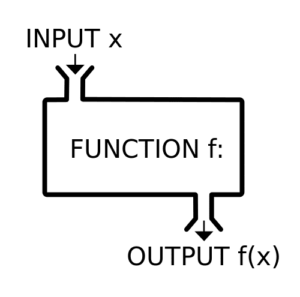
\includegraphics[width=1\linewidth]{images/function2} \end{center}

\begin{center}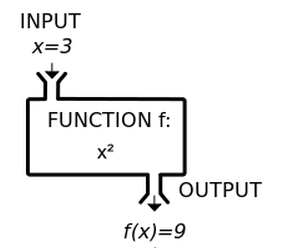
\includegraphics[width=1\linewidth]{images/function} \end{center}

Sintaxis

\begin{Shaded}
\begin{Highlighting}[]
\NormalTok{nombre.funcion }\OtherTok{\textless{}{-}} \ControlFlowTok{function}\NormalTok{(}\SpecialCharTok{\textless{}}\NormalTok{entradas}\SpecialCharTok{\textgreater{}}\NormalTok{)\{}
  
  \DocumentationTok{\#\#Cuerpo de la función}
  
\NormalTok{  return }\SpecialCharTok{\textless{}}\NormalTok{resultado}\SpecialCharTok{\textgreater{}}
  
\NormalTok{\}}
\end{Highlighting}
\end{Shaded}

\textbf{Ejemplos:}

\begin{Shaded}
\begin{Highlighting}[]
\DocumentationTok{\#\# Función que calcula el area de un triángulo dada su base y su altura.}


\CommentTok{\# Parámetros}
\DocumentationTok{\#\# base : Base del triángulo.}
\DocumentationTok{\#\# altura: Altura del triángulo}

\CommentTok{\# Resultado}
\DocumentationTok{\#\# area: Área del triángulo.}

\NormalTok{area.triangulo }\OtherTok{\textless{}{-}} \ControlFlowTok{function}\NormalTok{(base, altura) \{}
\NormalTok{  area }\OtherTok{\textless{}{-}}\NormalTok{ (base }\SpecialCharTok{*}\NormalTok{ altura) }\SpecialCharTok{/} \DecValTok{2}
  \FunctionTok{return}\NormalTok{(area)}
\NormalTok{\}}

\FunctionTok{area.triangulo}\NormalTok{(}\DecValTok{2}\NormalTok{, }\DecValTok{5}\NormalTok{)}
\end{Highlighting}
\end{Shaded}

\begin{verbatim}
## [1] 5
\end{verbatim}

Una persona desea sacar un préstamo, de \(P\) colones a una tasa de interés mensual \(i\). El préstamo tiene que ser reembolsado en \(n\) cuotas mensuales de tamaño \(C\), comenzando dentro de un mes. El problema es calcular \(C\). La fórmula \(C\) es:

\[
C = P\cdot\bigg(\dfrac{i}{1-(1+i)^{-n}}\bigg)
\]

Supongamos que \(P=150000\), que la tasa de interés es del \(2\%\) y que le número de pagos es \(10\). EL código en \textbf{R} sería:

\begin{Shaded}
\begin{Highlighting}[]
\NormalTok{tasa.interes }\OtherTok{\textless{}{-}} \FloatTok{0.02}
\NormalTok{n }\OtherTok{\textless{}{-}} \DecValTok{10}
\NormalTok{principal }\OtherTok{\textless{}{-}} \DecValTok{150000}
\NormalTok{pago }\OtherTok{\textless{}{-}}\NormalTok{ principal }\SpecialCharTok{*}\NormalTok{ tasa.interes }\SpecialCharTok{/}\NormalTok{ (}\DecValTok{1} \SpecialCharTok{{-}}\NormalTok{ (}\DecValTok{1} \SpecialCharTok{+}\NormalTok{ tasa.interes)}\SpecialCharTok{\^{}}\NormalTok{(}\SpecialCharTok{{-}}\NormalTok{n))}
\NormalTok{pago}
\end{Highlighting}
\end{Shaded}

\begin{verbatim}
## [1] 16698.98
\end{verbatim}

Utilizando una función:

\begin{Shaded}
\begin{Highlighting}[]
\CommentTok{\# Parámetros}
\DocumentationTok{\#\# tasa.interes : Tasa de interés mensual del préstamo}
\DocumentationTok{\#\# n: Número de cuotas}
\DocumentationTok{\#\# principal: Monto del préstamo}

\CommentTok{\# Resultado}
\DocumentationTok{\#\# pago: Cuota del préstamo.}


\NormalTok{calcula.cuota }\OtherTok{\textless{}{-}} \ControlFlowTok{function}\NormalTok{(tasa.interes, n, principal) \{}
\NormalTok{  pago }\OtherTok{\textless{}{-}}\NormalTok{ principal }\SpecialCharTok{*}\NormalTok{ tasa.interes }\SpecialCharTok{/}\NormalTok{ (}\DecValTok{1} \SpecialCharTok{{-}}\NormalTok{ (}\DecValTok{1} \SpecialCharTok{+}\NormalTok{ tasa.interes)}\SpecialCharTok{\^{}}\NormalTok{(}\SpecialCharTok{{-}}\NormalTok{n))}
  \FunctionTok{return}\NormalTok{(pago)}
\NormalTok{\}}


\FunctionTok{calcula.cuota}\NormalTok{(}\FloatTok{0.02}\NormalTok{, }\DecValTok{10}\NormalTok{, }\DecValTok{150000}\NormalTok{) }\DocumentationTok{\#\# Orden por defecto}
\end{Highlighting}
\end{Shaded}

\begin{verbatim}
## [1] 16698.98
\end{verbatim}

\begin{Shaded}
\begin{Highlighting}[]
\FunctionTok{calcula.cuota}\NormalTok{(}\AttributeTok{n =} \DecValTok{340}\NormalTok{, }\AttributeTok{tasa.interes =} \FloatTok{0.11}\NormalTok{, }\AttributeTok{principal =} \DecValTok{3500000}\NormalTok{) }\DocumentationTok{\#\# Para cambiar el orden se especifica el nombre del parámetro}
\end{Highlighting}
\end{Shaded}

\begin{verbatim}
## [1] 385000
\end{verbatim}

Ejemplo de función que retorna una lista.

\begin{Shaded}
\begin{Highlighting}[]
\CommentTok{\# Parámetros}
\DocumentationTok{\#\# DF : Data frame}
\DocumentationTok{\#\# NC: Número de columna}

\CommentTok{\# Resultado}
\DocumentationTok{\#\# lista con nombre de la variable correspondiente al número de columna, la media, la mediana, la desviación estándar,la varianza, el máximo y el mínimo.}

\NormalTok{estadisticas }\OtherTok{\textless{}{-}} \ControlFlowTok{function}\NormalTok{(DF, NC) \{}

\NormalTok{  variable }\OtherTok{\textless{}{-}}\NormalTok{ DF[, NC]}
\NormalTok{  nombre }\OtherTok{\textless{}{-}} \FunctionTok{colnames}\NormalTok{(DF)[NC]}

\NormalTok{  media }\OtherTok{\textless{}{-}} \FunctionTok{mean}\NormalTok{(variable)}
\NormalTok{  mediana }\OtherTok{\textless{}{-}} \FunctionTok{median}\NormalTok{(variable)}
\NormalTok{  deviacion }\OtherTok{\textless{}{-}} \FunctionTok{sd}\NormalTok{(variable)}
\NormalTok{  varianza }\OtherTok{\textless{}{-}} \FunctionTok{var}\NormalTok{(variable)}
\NormalTok{  maximo }\OtherTok{\textless{}{-}} \FunctionTok{max}\NormalTok{(variable)}
\NormalTok{  minimo }\OtherTok{\textless{}{-}} \FunctionTok{min}\NormalTok{(variable)}

  \FunctionTok{return}\NormalTok{(}\FunctionTok{list}\NormalTok{(}\AttributeTok{Variable =}\NormalTok{ nombre, }\AttributeTok{Media =}\NormalTok{ media, }\AttributeTok{Mediana =}\NormalTok{ mediana, }\AttributeTok{DesEst =}\NormalTok{ deviacion, }\AttributeTok{Varianza =}\NormalTok{ varianza, }\AttributeTok{Maximo =}\NormalTok{ maximo, }\AttributeTok{Minimo =}\NormalTok{ minimo))}
\NormalTok{\}}


\FunctionTok{estadisticas}\NormalTok{(portafolio.banco, }\DecValTok{20}\NormalTok{)}
\end{Highlighting}
\end{Shaded}

\begin{verbatim}
## Error in estadisticas(portafolio.banco, 20): object 'portafolio.banco' not found
\end{verbatim}

\hypertarget{importaciuxf3n-de-datos}{%
\chapter{\texorpdfstring{\textbf{Importación de datos}}{Importación de datos}}\label{importaciuxf3n-de-datos}}

Algunas de las funciones base en R para la lectura datos son:

\begin{itemize}
\tightlist
\item
  \textbf{read.table} , \textbf{read.csv}, se utilizan para leer datos que tienen formato de tabla.
\end{itemize}

\hypertarget{read.table}{%
\subsection{\texorpdfstring{\textbf{read.table}}{read.table}}\label{read.table}}

\begin{Shaded}
\begin{Highlighting}[]
\FunctionTok{read.table}\NormalTok{(}\AttributeTok{file =}\NormalTok{ archivo[, }\AttributeTok{header =} \ConstantTok{TRUE} \SpecialCharTok{|} \ConstantTok{FALSE}\NormalTok{,}
  \AttributeTok{sep =}\NormalTok{ separadorDatos, }\AttributeTok{dec =}\NormalTok{ separadorDecimal,}
  \AttributeTok{quote =}\NormalTok{ delimitadorCadenas,}
  \AttributeTok{stringsAsFactors =} \ConstantTok{TRUE} \SpecialCharTok{|} \ConstantTok{FALSE}\NormalTok{])}
\end{Highlighting}
\end{Shaded}

Esta es la función genérica para leer datos en formato .csv y genera , algunos de sus argumentos son:

\begin{itemize}
\tightlist
\item
  \textbf{file}: El nombre del archivo o su ubicación.
\item
  \textbf{header}: Variable lógica que indica si el archivo tiene encabezado.
\item
  \textbf{sep}: String que indica como están separadas las columnas.
\item
  \textbf{dec}: Para datos numéricos, establece cuál es el separador entre parte entera
  y decimal.
\item
  \textbf{colClasses}: Vector con las clases de cada una de las columnas.
\item
  \textbf{stringsAsFactors}: Indica si las variables de tipo character se deben leer como factor.
\end{itemize}

\textbf{Leer documentación de la función read.table}.

\hypertarget{read.csv}{%
\subsection{\texorpdfstring{\textbf{read.csv}}{read.csv}}\label{read.csv}}

Es una implementación especializada de read.table() en la que se asume
que los parámetros header, sep y dec toman los valores TRUE, ``,'' y ``.'' respectivamente.

\begin{Shaded}
\begin{Highlighting}[]
\NormalTok{datos.credito }\OtherTok{\textless{}{-}} \FunctionTok{read.csv}\NormalTok{(}\StringTok{"data/DeudaCredito.csv"}\NormalTok{, }\AttributeTok{sep =} \StringTok{";"}\NormalTok{, }\AttributeTok{dec =} \StringTok{"."}\NormalTok{)}

\FunctionTok{str}\NormalTok{(datos.credito)}
\end{Highlighting}
\end{Shaded}

\begin{verbatim}
## 'data.frame':    400 obs. of  13 variables:
##  $ X            : int  1 2 3 4 5 6 7 8 9 10 ...
##  $ monto_ingreso: num  14891 106025 104593 148924 55882 ...
##  $ monto_limite : int  3606 6645 7075 9504 4897 8047 3388 7114 3300 6819 ...
##  $ CalifCredit  : int  283 483 514 681 357 569 259 512 266 491 ...
##  $ Tarjetas     : int  2 3 4 3 2 4 2 2 5 3 ...
##  $ Edad         : int  34 82 71 36 68 77 37 87 66 41 ...
##  $ Educacion    : int  11 15 11 11 16 10 12 9 13 19 ...
##  $ Genero       : chr  "Masculino" "Femenino" "Masculino" "Femenino" ...
##  $ Estudiante   : chr  "No" "Si" "No" "No" ...
##  $ Casado       : int  1 1 0 0 1 0 0 0 0 1 ...
##  $ Etnicidad    : chr  "Caucasico" "Asiatico" "Asiatico" "Asiatico" ...
##  $ monto_balance: int  333 903 580 964 331 1151 203 872 279 1350 ...
##  $ fecha_ini    : chr  "12/11/2019" "12/13/2019" "12/17/2019" "12/06/2019" ...
\end{verbatim}

Podemos ver que varias variables que deberían ser categóricas se leyeron como strings, para corregir esto podemos colocar el parámetro \textbf{stringsAsFactors} igual a TRUE de la función read\_excel(), para leer los caracteres como factores.

\begin{Shaded}
\begin{Highlighting}[]
\NormalTok{datos.credito }\OtherTok{\textless{}{-}} \FunctionTok{read.csv}\NormalTok{(}\StringTok{"data/DeudaCredito.csv"}\NormalTok{, }\AttributeTok{sep =} \StringTok{","}\NormalTok{, }\AttributeTok{dec =} \StringTok{"."}\NormalTok{, }\AttributeTok{stringsAsFactors =}\NormalTok{ T)}

\FunctionTok{str}\NormalTok{(datos.credito)}
\end{Highlighting}
\end{Shaded}

\begin{verbatim}
## 'data.frame':    400 obs. of  12 variables:
##  $ X          : int  1 2 3 4 5 6 7 8 9 10 ...
##  $ Ingreso    : num  14.9 106 104.6 148.9 55.9 ...
##  $ Limite     : int  3606 6645 7075 9504 4897 8047 3388 7114 3300 6819 ...
##  $ CalifCredit: int  283 483 514 681 357 569 259 512 266 491 ...
##  $ Tarjetas   : int  2 3 4 3 2 4 2 2 5 3 ...
##  $ Edad       : int  34 82 71 36 68 77 37 87 66 41 ...
##  $ Educacion  : int  11 15 11 11 16 10 12 9 13 19 ...
##  $ Genero     : Factor w/ 2 levels "Femenino","Masculino": 2 1 2 1 2 2 1 2 1 1 ...
##  $ Estudiante : Factor w/ 2 levels "No","Si": 1 2 1 1 1 1 1 1 1 2 ...
##  $ Casado     : int  1 1 0 0 1 0 0 0 0 1 ...
##  $ Etnicidad  : Factor w/ 3 levels "Afrodescendiente",..: 3 2 2 2 3 3 1 2 3 1 ...
##  $ Balance    : int  333 903 580 964 331 1151 203 872 279 1350 ...
\end{verbatim}

\hypertarget{read_excel}{%
\subsection{\texorpdfstring{\textbf{read\_excel}}{read\_excel}}\label{read_excel}}

Esta se utiliza para leer datos de excel, algunos de sus argumentos son:

\begin{itemize}
\tightlist
\item
  \textbf{path}: Ruta del archivo.
\item
  \textbf{sheet}: Hoja del excel que se desea leer, por defecto es la primera.
\item
  \textbf{range}: Rango de celdas que se desean leer.
\item
  \textbf{col\_types}: Vector con las clases de cada una de las columnas.
\item
  \textbf{col\_names}: Indica si la primera fila corresponde al nombre de las columnas.
\end{itemize}

\begin{Shaded}
\begin{Highlighting}[]
\FunctionTok{library}\NormalTok{(readxl)}


\NormalTok{tipo\_cambio }\OtherTok{\textless{}{-}} \FunctionTok{read\_excel}\NormalTok{(}\StringTok{"data/tipo\_cambio.xls"}\NormalTok{)}

\NormalTok{tipo\_cambio\_top10 }\OtherTok{\textless{}{-}} \FunctionTok{head}\NormalTok{(tipo\_cambio, }\DecValTok{10}\NormalTok{) }\DocumentationTok{\#\# head(data,n) retorna las primeras n filas de nuestro data frame}

\NormalTok{tipo\_cambio\_top10}
\end{Highlighting}
\end{Shaded}

\begin{verbatim}
## # A tibble: 10 x 3
##    `Tipo cambio de compra y de venta del dólar de lo~ ...2         ...3         
##    <chr>                                              <chr>        <chr>        
##  1 Referencia del Banco Central de Costa Rica         <NA>         <NA>         
##  2 En colones costarricenses                          <NA>         <NA>         
##  3 <NA>                                               <NA>         <NA>         
##  4 <NA>                                               TIPO CAMBIO~ TIPO DE CAMB~
##  5 1 Ene 2019                                         604.3899999~ 611.75       
##  6 2 Ene 2019                                         604.3899999~ 611.75       
##  7 3 Ene 2019                                         603.0099999~ 611.54999999~
##  8 4 Ene 2019                                         604.7699999~ 611.67999999~
##  9 5 Ene 2019                                         602.3999999~ 611.54999999~
## 10 6 Ene 2019                                         602.3999999~ 611.54999999~
\end{verbatim}

Aplicando el head(), podemos ver que la lectura del archivo no es correcta, para hacerlo de forma correcta podemos utilizar el parámetro range de la función read\_excel(), para decirle que celdas queremos leer, la notación es la mimsa que se utiliza en MS Excel.

\begin{Shaded}
\begin{Highlighting}[]
\NormalTok{tipo\_cambio }\OtherTok{\textless{}{-}} \FunctionTok{read\_excel}\NormalTok{(}\StringTok{"data/tipo\_cambio.xls"}\NormalTok{, }\AttributeTok{range =} \StringTok{"A6:C787"}\NormalTok{, }\AttributeTok{col\_names =} \FunctionTok{c}\NormalTok{(}\StringTok{"fecha"}\NormalTok{, }\StringTok{"compra"}\NormalTok{, }\StringTok{"venta"}\NormalTok{))}

\FunctionTok{head}\NormalTok{(tipo\_cambio)}
\end{Highlighting}
\end{Shaded}

\begin{verbatim}
## # A tibble: 6 x 3
##   fecha      compra venta
##   <chr>       <dbl> <dbl>
## 1 1 Ene 2019   604.  612.
## 2 2 Ene 2019   604.  612.
## 3 3 Ene 2019   603.  612.
## 4 4 Ene 2019   605.  612.
## 5 5 Ene 2019   602.  612.
## 6 6 Ene 2019   602.  612.
\end{verbatim}

\hypertarget{calculando-requisitos-de-memoria.}{%
\subsection{\texorpdfstring{\textbf{Calculando requisitos de memoria}.}{Calculando requisitos de memoria.}}\label{calculando-requisitos-de-memoria.}}

Si queremos leer un archivo con 1.500.000 filas y 120 columnas, donde todas son de tipo numérico, realizamos el siguiente cálculo

\begin{align*}
1,500,000\times120\times 8 (bytes)\\
=&1.44\times10^9 (bytes)\\
=&1.44\times10^9 / 2^{20} (MB)\\
=&1,373 (MB)\\
=&1.34 (GB)\\
\end{align*}

por lo general se necesita el doble de esto, por lo que necesitamos al menos 4GB de RAM en nuestra computadora.

\hypertarget{anuxe1lisis-exploratorio}{%
\chapter{\texorpdfstring{\textbf{Análisis exploratorio}}{Análisis exploratorio}}\label{anuxe1lisis-exploratorio}}

Salvo que lo hayamos creado nosotros mismos o estemos familiarizados con el conjunto de datos que carguemos a \textbf{R}
generalmente estamos interesados en obtener una idea general sobre su contenido.
Con este fin se aplican funciones de estadística descriptiva, conservando la estructura de los datos (columnas
que lo forman y su tipo, número de observaciones, etc.), para tener una idea general
sobre cada variable.

\hypertarget{informaciuxf3n-general.}{%
\subsection{\texorpdfstring{\textbf{Información general}.}{Información general.}}\label{informaciuxf3n-general.}}

Asumiendo que comenzamos a trabajar con un conjunto de datos desconocido, lo primero que
nos interesa es sera saber qué atributos contiene, cuántas observaciones hay, etc.

En secciones anteriores se definieron funciones como class() y typeof(), con las
que podemos conocer la clase de un objeto y su tipo.

La función \textbf{str()} aporta más información, incluyendo el número de variables y observaciones y algunos detalles
sobre cada una de las variables (columnas).

\begin{Shaded}
\begin{Highlighting}[]
\FunctionTok{class}\NormalTok{(datos.credito) }\CommentTok{\# Clase del objeto}
\end{Highlighting}
\end{Shaded}

\begin{verbatim}
## [1] "data.frame"
\end{verbatim}

\begin{Shaded}
\begin{Highlighting}[]
\CommentTok{\# Información sobre su estructura}

\FunctionTok{str}\NormalTok{(datos.credito)}
\end{Highlighting}
\end{Shaded}

\begin{verbatim}
## 'data.frame':    400 obs. of  12 variables:
##  $ X          : int  1 2 3 4 5 6 7 8 9 10 ...
##  $ Ingreso    : num  14.9 106 104.6 148.9 55.9 ...
##  $ Limite     : int  3606 6645 7075 9504 4897 8047 3388 7114 3300 6819 ...
##  $ CalifCredit: int  283 483 514 681 357 569 259 512 266 491 ...
##  $ Tarjetas   : int  2 3 4 3 2 4 2 2 5 3 ...
##  $ Edad       : int  34 82 71 36 68 77 37 87 66 41 ...
##  $ Educacion  : int  11 15 11 11 16 10 12 9 13 19 ...
##  $ Genero     : Factor w/ 2 levels "Femenino","Masculino": 2 1 2 1 2 2 1 2 1 1 ...
##  $ Estudiante : Factor w/ 2 levels "No","Si": 1 2 1 1 1 1 1 1 1 2 ...
##  $ Casado     : int  1 1 0 0 1 0 0 0 0 1 ...
##  $ Etnicidad  : Factor w/ 3 levels "Afrodescendiente",..: 3 2 2 2 3 3 1 2 3 1 ...
##  $ Balance    : int  333 903 580 964 331 1151 203 872 279 1350 ...
\end{verbatim}

\hypertarget{exploraciuxf3n-del-contenido.}{%
\subsection{\texorpdfstring{\textbf{Exploración del contenido}.}{Exploración del contenido.}}\label{exploraciuxf3n-del-contenido.}}

Aunque la función \textbf{str()} facilita una muestra del contenido de cada variable, en
general dicha información es insuficiente. Podemos recurrir a funciones
como \textbf{head()} y \textbf{tail()} para obtener los primeros y últimos elementos, respectivamente, de un objeto en \textbf{R}. Asimismo, la función \textbf{summary()} ofrece un resumen global del contenido de cada variable: su valor mínimo, máximo y medio, mediana, cuartiles
y, en el caso de las variables qualitativas, el número de elementos por categoría.

\begin{Shaded}
\begin{Highlighting}[]
\FunctionTok{head}\NormalTok{(datos.credito) }\DocumentationTok{\#\# head(X,n) muestra los primeros n elementos del objeto X, por defecto n=6.}
\end{Highlighting}
\end{Shaded}

\begin{verbatim}
##   X Ingreso Limite CalifCredit Tarjetas Edad Educacion    Genero Estudiante
## 1 1  14.891   3606         283        2   34        11 Masculino         No
## 2 2 106.025   6645         483        3   82        15  Femenino         Si
## 3 3 104.593   7075         514        4   71        11 Masculino         No
## 4 4 148.924   9504         681        3   36        11  Femenino         No
## 5 5  55.882   4897         357        2   68        16 Masculino         No
## 6 6  80.180   8047         569        4   77        10 Masculino         No
##   Casado Etnicidad Balance
## 1      1 Caucasico     333
## 2      1  Asiatico     903
## 3      0  Asiatico     580
## 4      0  Asiatico     964
## 5      1 Caucasico     331
## 6      0 Caucasico    1151
\end{verbatim}

\begin{Shaded}
\begin{Highlighting}[]
\FunctionTok{head}\NormalTok{(datos.credito, }\DecValTok{3}\NormalTok{)}
\end{Highlighting}
\end{Shaded}

\begin{verbatim}
##   X Ingreso Limite CalifCredit Tarjetas Edad Educacion    Genero Estudiante
## 1 1  14.891   3606         283        2   34        11 Masculino         No
## 2 2 106.025   6645         483        3   82        15  Femenino         Si
## 3 3 104.593   7075         514        4   71        11 Masculino         No
##   Casado Etnicidad Balance
## 1      1 Caucasico     333
## 2      1  Asiatico     903
## 3      0  Asiatico     580
\end{verbatim}

\begin{Shaded}
\begin{Highlighting}[]
\FunctionTok{tail}\NormalTok{(datos.credito)}
\end{Highlighting}
\end{Shaded}

\begin{verbatim}
##       X Ingreso Limite CalifCredit Tarjetas Edad Educacion    Genero Estudiante
## 395 395  49.794   5758         410        4   40         8 Masculino         No
## 396 396  12.096   4100         307        3   32        13 Masculino         No
## 397 397  13.364   3838         296        5   65        17 Masculino         No
## 398 398  57.872   4171         321        5   67        12  Femenino         No
## 399 399  37.728   2525         192        1   44        13 Masculino         No
## 400 400  18.701   5524         415        5   64         7  Femenino         No
##     Casado        Etnicidad Balance
## 395      0        Caucasico     734
## 396      1        Caucasico     560
## 397      0 Afrodescendiente     480
## 398      1        Caucasico     138
## 399      1        Caucasico       0
## 400      0         Asiatico     966
\end{verbatim}

\begin{Shaded}
\begin{Highlighting}[]
\FunctionTok{tail}\NormalTok{(datos.credito, }\DecValTok{3}\NormalTok{)}
\end{Highlighting}
\end{Shaded}

\begin{verbatim}
##       X Ingreso Limite CalifCredit Tarjetas Edad Educacion    Genero Estudiante
## 398 398  57.872   4171         321        5   67        12  Femenino         No
## 399 399  37.728   2525         192        1   44        13 Masculino         No
## 400 400  18.701   5524         415        5   64         7  Femenino         No
##     Casado Etnicidad Balance
## 398      1 Caucasico     138
## 399      1 Caucasico       0
## 400      0  Asiatico     966
\end{verbatim}

\begin{Shaded}
\begin{Highlighting}[]
\FunctionTok{summary}\NormalTok{(datos.credito)}
\end{Highlighting}
\end{Shaded}

\begin{verbatim}
##        X            Ingreso           Limite       CalifCredit   
##  Min.   :  1.0   Min.   : 10.35   Min.   :  855   Min.   : 93.0  
##  1st Qu.:100.8   1st Qu.: 21.01   1st Qu.: 3088   1st Qu.:247.2  
##  Median :200.5   Median : 33.12   Median : 4622   Median :344.0  
##  Mean   :200.5   Mean   : 45.22   Mean   : 4736   Mean   :354.9  
##  3rd Qu.:300.2   3rd Qu.: 57.47   3rd Qu.: 5873   3rd Qu.:437.2  
##  Max.   :400.0   Max.   :186.63   Max.   :13913   Max.   :982.0  
##     Tarjetas          Edad         Educacion           Genero    Estudiante
##  Min.   :1.000   Min.   :23.00   Min.   : 5.00   Femenino :207   No:360    
##  1st Qu.:2.000   1st Qu.:41.75   1st Qu.:11.00   Masculino:193   Si: 40    
##  Median :3.000   Median :56.00   Median :14.00                             
##  Mean   :2.958   Mean   :55.67   Mean   :13.45                             
##  3rd Qu.:4.000   3rd Qu.:70.00   3rd Qu.:16.00                             
##  Max.   :9.000   Max.   :98.00   Max.   :20.00                             
##      Casado                  Etnicidad      Balance       
##  Min.   :0.0000   Afrodescendiente: 99   Min.   :   0.00  
##  1st Qu.:0.0000   Asiatico        :102   1st Qu.:  68.75  
##  Median :1.0000   Caucasico       :199   Median : 459.50  
##  Mean   :0.6125                          Mean   : 520.01  
##  3rd Qu.:1.0000                          3rd Qu.: 863.00  
##  Max.   :1.0000                          Max.   :1999.00
\end{verbatim}

Como podemos observar la variable \textbf{Casado} se leyó como numérica, esto no tienen mucho sentido, para transformarla a categórica utilizamos la función factor().

\begin{Shaded}
\begin{Highlighting}[]
\DocumentationTok{\#\# Transformamos la variable Casado a categorica}

\NormalTok{datos.credito}\SpecialCharTok{$}\NormalTok{Casado }\OtherTok{\textless{}{-}} \FunctionTok{factor}\NormalTok{(datos.credito}\SpecialCharTok{$}\NormalTok{Casado, }\AttributeTok{levels =} \FunctionTok{c}\NormalTok{(}\DecValTok{1}\NormalTok{, }\DecValTok{0}\NormalTok{), }\AttributeTok{labels =} \FunctionTok{c}\NormalTok{(}\StringTok{"si"}\NormalTok{, }\StringTok{"no"}\NormalTok{))}
\FunctionTok{summary}\NormalTok{(datos.credito)}
\end{Highlighting}
\end{Shaded}

\begin{verbatim}
##        X            Ingreso           Limite       CalifCredit   
##  Min.   :  1.0   Min.   : 10.35   Min.   :  855   Min.   : 93.0  
##  1st Qu.:100.8   1st Qu.: 21.01   1st Qu.: 3088   1st Qu.:247.2  
##  Median :200.5   Median : 33.12   Median : 4622   Median :344.0  
##  Mean   :200.5   Mean   : 45.22   Mean   : 4736   Mean   :354.9  
##  3rd Qu.:300.2   3rd Qu.: 57.47   3rd Qu.: 5873   3rd Qu.:437.2  
##  Max.   :400.0   Max.   :186.63   Max.   :13913   Max.   :982.0  
##     Tarjetas          Edad         Educacion           Genero    Estudiante
##  Min.   :1.000   Min.   :23.00   Min.   : 5.00   Femenino :207   No:360    
##  1st Qu.:2.000   1st Qu.:41.75   1st Qu.:11.00   Masculino:193   Si: 40    
##  Median :3.000   Median :56.00   Median :14.00                             
##  Mean   :2.958   Mean   :55.67   Mean   :13.45                             
##  3rd Qu.:4.000   3rd Qu.:70.00   3rd Qu.:16.00                             
##  Max.   :9.000   Max.   :98.00   Max.   :20.00                             
##  Casado              Etnicidad      Balance       
##  si:245   Afrodescendiente: 99   Min.   :   0.00  
##  no:155   Asiatico        :102   1st Qu.:  68.75  
##           Caucasico       :199   Median : 459.50  
##                                  Mean   : 520.01  
##                                  3rd Qu.: 863.00  
##                                  Max.   :1999.00
\end{verbatim}

Por otro lado la variable fecha\_ini se leyó como factor, en lugar de como fecha, para corregir esto usamos la función as.Date().

\begin{Shaded}
\begin{Highlighting}[]
\NormalTok{datos.credito}\SpecialCharTok{$}\NormalTok{fecha\_ini }\OtherTok{\textless{}{-}} \FunctionTok{as.Date}\NormalTok{(datos.credito}\SpecialCharTok{$}\NormalTok{fecha\_ini, }\AttributeTok{format =} \StringTok{"\%m/\%d/\%Y"}\NormalTok{)}
\end{Highlighting}
\end{Shaded}

\begin{verbatim}
## Error in `$<-.data.frame`(`*tmp*`, fecha_ini, value = structure(numeric(0), class = "Date")): replacement has 0 rows, data has 400
\end{verbatim}

\hypertarget{funciones-buxe1sicas.}{%
\subsection{\texorpdfstring{\textbf{Funciones básicas}.}{Funciones básicas.}}\label{funciones-buxe1sicas.}}

Recordemos que \textbf{R} cuenta con multitud de funciones de tipo estadístico, entre ellas las que permiten
obtener información descriptiva sobre la distribución de valores en un vector. Estas
funciones pueden también aplicarse a objetos más complejos, como comprobaremos
después.
La sintaxis de las funciones de estadística descriptiva más comunes se presentan a continuación.

\begin{Shaded}
\begin{Highlighting}[]
\FunctionTok{min}\NormalTok{(vector, }\AttributeTok{na.rm =}\NormalTok{ T }\SpecialCharTok{/}\NormalTok{ F) }\CommentTok{\# Devuelve el valor mínimo existente en el vector facilitado como parámetro.}

\CommentTok{\# El resultado será NA si el vector contiene algún valor ausente, a menos que se}
\CommentTok{\# entregue el parámetro na.rm con el valor TRUE.}
\end{Highlighting}
\end{Shaded}

\begin{Shaded}
\begin{Highlighting}[]
\FunctionTok{max}\NormalTok{(vector, }\AttributeTok{na.rm =}\NormalTok{ T }\SpecialCharTok{/}\NormalTok{ F) }\CommentTok{\# Devuelve el valor máximo existente en el vector facilitado como parámetro.}

\CommentTok{\# El resultado será NA si el vector contiene algún valor ausente, a menos que se}
\CommentTok{\# entregue el parámetro na.rm con el valor TRUE.}
\end{Highlighting}
\end{Shaded}

\begin{Shaded}
\begin{Highlighting}[]
\FunctionTok{range}\NormalTok{(vector, }\AttributeTok{na.rm =}\NormalTok{ T }\SpecialCharTok{/}\NormalTok{ F) }\CommentTok{\# Devuelve un vector de dos elementos con el valor mínimo y máximo de los}
\CommentTok{\# existentes en el vector facilitado como parámetro}
\end{Highlighting}
\end{Shaded}

\begin{Shaded}
\begin{Highlighting}[]
\FunctionTok{range}\NormalTok{(vector, }\AttributeTok{na.rm =}\NormalTok{ T }\SpecialCharTok{/}\NormalTok{ F) }\CommentTok{\# Devuelve un vector de dos elementos con el valor mínimo y máximo de los}
\CommentTok{\# existentes en el vector facilitado como parámetro}
\end{Highlighting}
\end{Shaded}

\begin{Shaded}
\begin{Highlighting}[]
\NormalTok{saldo }\OtherTok{\textless{}{-}} \FunctionTok{c}\NormalTok{(}\DecValTok{1000}\NormalTok{, }\DecValTok{2000}\NormalTok{, }\DecValTok{3000}\NormalTok{, }\DecValTok{4500}\NormalTok{)}

\FunctionTok{min}\NormalTok{(saldo)}
\end{Highlighting}
\end{Shaded}

\begin{verbatim}
## [1] 1000
\end{verbatim}

\begin{Shaded}
\begin{Highlighting}[]
\FunctionTok{max}\NormalTok{(saldo)}
\end{Highlighting}
\end{Shaded}

\begin{verbatim}
## [1] 4500
\end{verbatim}

\begin{Shaded}
\begin{Highlighting}[]
\FunctionTok{range}\NormalTok{(saldo)}
\end{Highlighting}
\end{Shaded}

\begin{verbatim}
## [1] 1000 4500
\end{verbatim}

\begin{Shaded}
\begin{Highlighting}[]
\FunctionTok{mean}\NormalTok{(saldo)}
\end{Highlighting}
\end{Shaded}

\begin{verbatim}
## [1] 2625
\end{verbatim}

\begin{Shaded}
\begin{Highlighting}[]
\FunctionTok{var}\NormalTok{(saldo)}
\end{Highlighting}
\end{Shaded}

\begin{verbatim}
## [1] 2229167
\end{verbatim}

\begin{Shaded}
\begin{Highlighting}[]
\FunctionTok{sd}\NormalTok{(saldo)}
\end{Highlighting}
\end{Shaded}

\begin{verbatim}
## [1] 1493.039
\end{verbatim}

\begin{Shaded}
\begin{Highlighting}[]
\FunctionTok{median}\NormalTok{(saldo)}
\end{Highlighting}
\end{Shaded}

\begin{verbatim}
## [1] 2500
\end{verbatim}

\begin{Shaded}
\begin{Highlighting}[]
\FunctionTok{quantile}\NormalTok{(saldo)}
\end{Highlighting}
\end{Shaded}

\begin{verbatim}
##   0%  25%  50%  75% 100% 
## 1000 1750 2500 3375 4500
\end{verbatim}

A fin de obtener un resultado más compacto,
se crea una lista con el valor devuelto por cada operación y, finalmente, se usa la
función \textbf{unlist()} para generar un vector con la información a mostrar:

\begin{Shaded}
\begin{Highlighting}[]
\NormalTok{valores }\OtherTok{\textless{}{-}}\NormalTok{ saldo}
\FunctionTok{unlist}\NormalTok{(}\FunctionTok{list}\NormalTok{(}\AttributeTok{media =} \FunctionTok{mean}\NormalTok{(valores), }\AttributeTok{desviacion =} \FunctionTok{sd}\NormalTok{(valores), }\AttributeTok{varianza =} \FunctionTok{var}\NormalTok{(valores), }\AttributeTok{minimo =} \FunctionTok{min}\NormalTok{(valores), }\AttributeTok{maximo =} \FunctionTok{max}\NormalTok{(valores), }\AttributeTok{mediana =} \FunctionTok{median}\NormalTok{(valores), }\AttributeTok{rango =} \FunctionTok{range}\NormalTok{(valores), }\AttributeTok{quartiles =} \FunctionTok{quantile}\NormalTok{(valores)))}
\end{Highlighting}
\end{Shaded}

\begin{verbatim}
##          media     desviacion       varianza         minimo         maximo 
##       2625.000       1493.039    2229166.667       1000.000       4500.000 
##        mediana         rango1         rango2   quartiles.0%  quartiles.25% 
##       2500.000       1000.000       4500.000       1000.000       1750.000 
##  quartiles.50%  quartiles.75% quartiles.100% 
##       2500.000       3375.000       4500.000
\end{verbatim}

\hypertarget{aplicaciuxf3n-a-estructuras-complejas.}{%
\subsection{\texorpdfstring{\textbf{Aplicación a estructuras complejas}.}{Aplicación a estructuras complejas.}}\label{aplicaciuxf3n-a-estructuras-complejas.}}

Las anteriores funciones pueden aplicarse sobre estructuras más complejas que
los vectores, como matrices y data frames. En la mayoría de los casos no nos interesan las medidas estadísticas de todo el conjunto de datos, sino de cada una de las variables (columnas) por separado.

\begin{Shaded}
\begin{Highlighting}[]
\FunctionTok{mean}\NormalTok{(datos.credito}\SpecialCharTok{$}\NormalTok{Ingreso)}
\end{Highlighting}
\end{Shaded}

\begin{verbatim}
## [1] 45.21889
\end{verbatim}

\begin{Shaded}
\begin{Highlighting}[]
\FunctionTok{max}\NormalTok{(datos.credito}\SpecialCharTok{$}\NormalTok{Limite)}
\end{Highlighting}
\end{Shaded}

\begin{verbatim}
## [1] 13913
\end{verbatim}

\hypertarget{data-frames-con-el-paquete-dplyr.}{%
\chapter{\texorpdfstring{\textbf{Data Frames con el paquete dplyr.}}{Data Frames con el paquete dplyr.}}\label{data-frames-con-el-paquete-dplyr.}}

Como vimos en la clase anterior los data frames son las estructuras más importantes en R, recordemos que básicamente un data frame es una tabla, donde cada fila representa una observación o individuo, y cada columna una variable o característica de esta observación.

Dada la importancia de estas estructuras, es muy importante conocer las mejores herramientas para trabajar con ellas, en la sección de
subsetting vimos como obtener subconjuntos de nuestros datos, sin embargo cuando tenemos que hacer varios filtros o agrupaciones el uso de ``{[}{]},'' ``\$,'' no es tan recomendable, pues es más fácil equivocarse y el código es más complicado de leer.

El paquete \textbf{dplyr} está diseñado para mitigar estas complicaciones y optimizado para realizar estas tareas.

\hypertarget{paquete-dplyr}{%
\section{\texorpdfstring{\textbf{Paquete dplyr}:}{Paquete dplyr:}}\label{paquete-dplyr}}

El paquete \textbf{dplyr} fue desarrollado por Hadley Wickham de RStudio y us una versión mejorada del paquete \textbf{plyr}. Una de las ventajas de este paquete es que tiene cierta gramática en sus funciones, lo que facilita escribir y leer código. Además sus funciones son muy rápidas y algunas de sus operaciones están programadas en C++.

\textbf{Gramática de dplyr}

Algunos de los ``verbos'' que tiene el paquete \textbf{dplyr} son los siguientes:

\begin{itemize}
\tightlist
\item
  \textbf{select}: Retorna un subconjunto de columnas.
\item
  \textbf{filter}: Extrae subconjuntos de filas basado en condiciones lógicas.
\item
  \textbf{arrange}: Reordena las filas de un data frame.
\item
  \textbf{rename}: Renombra las variables del data frame.
\item
  \textbf{mutate}: Agrega columnas o transforma las existentes.
\item
  \textbf{summarise / summarize}: Genera un resumen estadístico de las variables del data frame.
\item
  \textbf{\%\textgreater\%}: El operador ``pipe'' es usado para conectar varios ``verbos'' en una sola ejecución.
\end{itemize}

Es importante notar que, el primer argumento de todas estas funciones es un data frame y su resultado también es un data frame, por eso es fácil y útil combinarlas.

\textbf{Instalación}

\begin{Shaded}
\begin{Highlighting}[]
\DocumentationTok{\#\# Para instalarlo basta ejecutar lo siguiente en la consola}
\FunctionTok{install.packages}\NormalTok{(}\StringTok{"dplyr"}\NormalTok{)}

\DocumentationTok{\#\# Para utilizar las funciones se debe cargar la librería mediante la instrucción}
\FunctionTok{library}\NormalTok{(dplyr)}
\end{Highlighting}
\end{Shaded}

Cargamos el archivo de datos

\begin{Shaded}
\begin{Highlighting}[]
\NormalTok{datos.credito }\OtherTok{\textless{}{-}} \FunctionTok{read.csv}\NormalTok{(}\StringTok{"data/DeudaCredito.csv"}\NormalTok{, }\AttributeTok{sep =} \StringTok{";"}\NormalTok{, }\AttributeTok{dec =} \StringTok{"."}\NormalTok{, }\AttributeTok{stringsAsFactors =}\NormalTok{ T)}

\NormalTok{datos.credito}\SpecialCharTok{$}\NormalTok{Casado }\OtherTok{\textless{}{-}} \FunctionTok{factor}\NormalTok{(datos.credito}\SpecialCharTok{$}\NormalTok{Casado, }\AttributeTok{levels =} \FunctionTok{c}\NormalTok{(}\DecValTok{1}\NormalTok{, }\DecValTok{0}\NormalTok{), }\AttributeTok{labels =} \FunctionTok{c}\NormalTok{(}\StringTok{"si"}\NormalTok{, }\StringTok{"no"}\NormalTok{))}

\NormalTok{datos.credito}\SpecialCharTok{$}\NormalTok{fecha\_ini }\OtherTok{\textless{}{-}} \FunctionTok{as.Date}\NormalTok{(datos.credito}\SpecialCharTok{$}\NormalTok{fecha\_ini, }\AttributeTok{format =} \StringTok{"\%m/\%d/\%Y"}\NormalTok{)}
\end{Highlighting}
\end{Shaded}

\hypertarget{select}{%
\section{\texorpdfstring{\textbf{select()}:}{select():}}\label{select}}

Normalmente trabajamos con data frames que tienen muchas variables y necesitamos enfocarnos en solo algunas de estas, la función \textbf{select()} como su nombre lo sugiere, sirve para obtener las columnas deseadas de nuestro conjunto de datos.

Primero vamos a ver de forma general la estructura de nuestros datos, utilizando las funciones \textbf{dim()
} y \textbf{str()}.

\begin{Shaded}
\begin{Highlighting}[]
\FunctionTok{dim}\NormalTok{(datos.credito) }\DocumentationTok{\#\# Obtenemos la dimensiones de nuestro data frame [filas, columnas].}
\end{Highlighting}
\end{Shaded}

\begin{verbatim}
## [1] 400  13
\end{verbatim}

\begin{Shaded}
\begin{Highlighting}[]
\FunctionTok{str}\NormalTok{(datos.credito) }\DocumentationTok{\#\# Presenta un resumen las variables del data frame y su clase.}
\end{Highlighting}
\end{Shaded}

\begin{verbatim}
## 'data.frame':    400 obs. of  13 variables:
##  $ X            : int  1 2 3 4 5 6 7 8 9 10 ...
##  $ monto_ingreso: num  14891 106025 104593 148924 55882 ...
##  $ monto_limite : int  3606 6645 7075 9504 4897 8047 3388 7114 3300 6819 ...
##  $ CalifCredit  : int  283 483 514 681 357 569 259 512 266 491 ...
##  $ Tarjetas     : int  2 3 4 3 2 4 2 2 5 3 ...
##  $ Edad         : int  34 82 71 36 68 77 37 87 66 41 ...
##  $ Educacion    : int  11 15 11 11 16 10 12 9 13 19 ...
##  $ Genero       : Factor w/ 2 levels "Femenino","Masculino": 2 1 2 1 2 2 1 2 1 1 ...
##  $ Estudiante   : Factor w/ 2 levels "No","Si": 1 2 1 1 1 1 1 1 1 2 ...
##  $ Casado       : Factor w/ 2 levels "si","no": 1 1 2 2 1 2 2 2 2 1 ...
##  $ Etnicidad    : Factor w/ 3 levels "Afrodescendiente",..: 3 2 2 2 3 3 1 2 3 1 ...
##  $ monto_balance: int  333 903 580 964 331 1151 203 872 279 1350 ...
##  $ fecha_ini    : Date, format: "2019-12-11" "2019-12-13" ...
\end{verbatim}

Suponga que queremos las columnas Edad, Educación, Género, Estudiante, Casado

\begin{Shaded}
\begin{Highlighting}[]
\NormalTok{datos.credito.info\_personal }\OtherTok{\textless{}{-}} \FunctionTok{select}\NormalTok{(datos.credito, }\FunctionTok{c}\NormalTok{(}\StringTok{"Edad"}\NormalTok{, }\StringTok{"Educacion"}\NormalTok{, }\StringTok{"Genero"}\NormalTok{, }\StringTok{"Estudiante"}\NormalTok{, }\StringTok{"Casado"}\NormalTok{, }\StringTok{"Etnicidad"}\NormalTok{))}

\FunctionTok{head}\NormalTok{(datos.credito.info\_personal)}
\end{Highlighting}
\end{Shaded}

\begin{verbatim}
##   Edad Educacion    Genero Estudiante Casado Etnicidad
## 1   34        11 Masculino         No     si Caucasico
## 2   82        15  Femenino         Si     si  Asiatico
## 3   71        11 Masculino         No     no  Asiatico
## 4   36        11  Femenino         No     no  Asiatico
## 5   68        16 Masculino         No     si Caucasico
## 6   77        10 Masculino         No     no Caucasico
\end{verbatim}

También podemos utilizar el \textbf{select()} eligiendo las columnas que no queremos.

\begin{Shaded}
\begin{Highlighting}[]
\NormalTok{datos.credito.info\_personal.sinEtnia }\OtherTok{\textless{}{-}} \FunctionTok{select}\NormalTok{(datos.credito.info\_personal, }\SpecialCharTok{{-}}\NormalTok{Etnicidad)  }\DocumentationTok{\#\# para quitar varias columnas utilizamos un vector, por ejemplo: {-}c("Etnicidad", "Casado)}

\FunctionTok{head}\NormalTok{(datos.credito.info\_personal.sinEtnia)}
\end{Highlighting}
\end{Shaded}

\begin{verbatim}
##   Edad Educacion    Genero Estudiante Casado
## 1   34        11 Masculino         No     si
## 2   82        15  Femenino         Si     si
## 3   71        11 Masculino         No     no
## 4   36        11  Femenino         No     no
## 5   68        16 Masculino         No     si
## 6   77        10 Masculino         No     no
\end{verbatim}

Otra forma es seleccionar las columnas que tengan inicien o terminen con ciertos caracteres, por ejemplo si queremos todas las columnas que tienen el prefijo ``monto.''

\begin{Shaded}
\begin{Highlighting}[]
\NormalTok{datos.credito\_montos }\OtherTok{\textless{}{-}} \FunctionTok{select}\NormalTok{(datos.credito, }\FunctionTok{starts\_with}\NormalTok{(}\StringTok{"monto"}\NormalTok{)) }\DocumentationTok{\#\# Podemos usar ends\_with("sufijo") para elegir las que terminen con cierto sufijo.}

\FunctionTok{head}\NormalTok{(datos.credito\_montos)}
\end{Highlighting}
\end{Shaded}

\begin{verbatim}
##   monto_ingreso monto_limite monto_balance
## 1      14891.00         3606           333
## 2     106025.00         6645           903
## 3     104593.00         7075           580
## 4     148924.00         9504           964
## 5      55882.00         4897           331
## 6         80.18         8047          1151
\end{verbatim}

\hypertarget{filter}{%
\section{\texorpdfstring{\textbf{filter()}:}{filter():}}\label{filter}}

Esta función se utiliza para extraer filas de nuestro data frame utilizando condiciones.

\begin{Shaded}
\begin{Highlighting}[]
\NormalTok{datos.credito\_enero }\OtherTok{\textless{}{-}} \FunctionTok{filter}\NormalTok{(datos.credito, }\FunctionTok{months}\NormalTok{(fecha\_ini) }\SpecialCharTok{==} \StringTok{"January"}\NormalTok{)}

\FunctionTok{dim}\NormalTok{(datos.credito\_enero)}
\end{Highlighting}
\end{Shaded}

\begin{verbatim}
## [1]  0 13
\end{verbatim}

\begin{Shaded}
\begin{Highlighting}[]
\FunctionTok{head}\NormalTok{(datos.credito\_enero)}
\end{Highlighting}
\end{Shaded}

\begin{verbatim}
##  [1] X             monto_ingreso monto_limite  CalifCredit   Tarjetas     
##  [6] Edad          Educacion     Genero        Estudiante    Casado       
## [11] Etnicidad     monto_balance fecha_ini    
## <0 rows> (or 0-length row.names)
\end{verbatim}

\begin{Shaded}
\begin{Highlighting}[]
\NormalTok{datos.credito\_enero\_fem }\OtherTok{\textless{}{-}} \FunctionTok{filter}\NormalTok{(datos.credito, }\FunctionTok{months}\NormalTok{(fecha\_ini) }\SpecialCharTok{==} \StringTok{"January"} \SpecialCharTok{\&}\NormalTok{ Genero }\SpecialCharTok{==} \StringTok{"Femenino"}\NormalTok{)}

\FunctionTok{dim}\NormalTok{(datos.credito\_enero\_fem)}
\end{Highlighting}
\end{Shaded}

\begin{verbatim}
## [1]  0 13
\end{verbatim}

\begin{Shaded}
\begin{Highlighting}[]
\FunctionTok{head}\NormalTok{(datos.credito\_enero\_fem)}
\end{Highlighting}
\end{Shaded}

\begin{verbatim}
##  [1] X             monto_ingreso monto_limite  CalifCredit   Tarjetas     
##  [6] Edad          Educacion     Genero        Estudiante    Casado       
## [11] Etnicidad     monto_balance fecha_ini    
## <0 rows> (or 0-length row.names)
\end{verbatim}

\hypertarget{arrange}{%
\section{\texorpdfstring{\textbf{arrange()}:}{arrange():}}\label{arrange}}

Esta función se utiliza para ordenar las filas de un data frame de acuerdo a una de sus variables.

Ordenamos de acuerdo la columna que contiene las fechas de inicio.

\begin{Shaded}
\begin{Highlighting}[]
\NormalTok{datos.credito\_ordenado }\OtherTok{\textless{}{-}} \FunctionTok{arrange}\NormalTok{(datos.credito, fecha\_ini) }\DocumentationTok{\#\# De forma ascendente por defecto}

\FunctionTok{head}\NormalTok{(}\FunctionTok{select}\NormalTok{(datos.credito\_ordenado, fecha\_ini, monto\_balance))}
\end{Highlighting}
\end{Shaded}

\begin{verbatim}
##    fecha_ini monto_balance
## 1 2011-01-17          1448
## 2 2016-06-01             0
## 3 2016-10-21           962
## 4 2016-10-21           345
## 5 2016-10-21             0
## 6 2016-10-21           480
\end{verbatim}

\begin{Shaded}
\begin{Highlighting}[]
\NormalTok{datos.credito\_ordenado }\OtherTok{\textless{}{-}} \FunctionTok{arrange}\NormalTok{(datos.credito, }\FunctionTok{desc}\NormalTok{(fecha\_ini)) }\DocumentationTok{\#\# De forma descendente.}

\FunctionTok{head}\NormalTok{(}\FunctionTok{select}\NormalTok{(datos.credito\_ordenado, fecha\_ini, monto\_balance))}
\end{Highlighting}
\end{Shaded}

\begin{verbatim}
##    fecha_ini monto_balance
## 1 2020-06-30           250
## 2 2020-06-30           295
## 3 2020-06-29           637
## 4 2020-06-29           209
## 5 2020-06-29           531
## 6 2020-06-26             0
\end{verbatim}

\hypertarget{rename}{%
\section{\texorpdfstring{\textbf{rename()}:}{rename():}}\label{rename}}

Renombrar variables puede ser de mucha utilidad para poder escribir código y hacerlo más legible. Sin la función \textbf{rename()} esta tarea puede ser bastante tediosa.

\begin{Shaded}
\begin{Highlighting}[]
\NormalTok{datos.credito }\OtherTok{\textless{}{-}} \FunctionTok{rename}\NormalTok{(datos.credito, }\AttributeTok{cant\_tarjetas =} \StringTok{"Tarjetas"}\NormalTok{, }\AttributeTok{calif\_credit =}\NormalTok{ CalifCredit, }\AttributeTok{id =}\NormalTok{ X)}

\FunctionTok{head}\NormalTok{(datos.credito)}
\end{Highlighting}
\end{Shaded}

\begin{verbatim}
##   id monto_ingreso monto_limite calif_credit cant_tarjetas Edad Educacion
## 1  1      14891.00         3606          283             2   34        11
## 2  2     106025.00         6645          483             3   82        15
## 3  3     104593.00         7075          514             4   71        11
## 4  4     148924.00         9504          681             3   36        11
## 5  5      55882.00         4897          357             2   68        16
## 6  6         80.18         8047          569             4   77        10
##      Genero Estudiante Casado Etnicidad monto_balance  fecha_ini
## 1 Masculino         No     si Caucasico           333 2019-12-11
## 2  Femenino         Si     si  Asiatico           903 2019-12-13
## 3 Masculino         No     no  Asiatico           580 2019-12-17
## 4  Femenino         No     no  Asiatico           964 2019-12-06
## 5 Masculino         No     si Caucasico           331 2019-10-17
## 6 Masculino         No     no Caucasico          1151 2020-02-07
\end{verbatim}

\hypertarget{mutate}{%
\section{\texorpdfstring{\textbf{mutate()}:}{mutate():}}\label{mutate}}

Esta función nos permite crear variables a partir de las que ya existen, de una forma muy sencilla.

\begin{Shaded}
\begin{Highlighting}[]
\NormalTok{datos.credito }\OtherTok{\textless{}{-}} \FunctionTok{mutate}\NormalTok{(datos.credito, }\AttributeTok{razon =}\NormalTok{ monto\_limite }\SpecialCharTok{/}\NormalTok{ monto\_ingreso)}

\FunctionTok{head}\NormalTok{(}\FunctionTok{select}\NormalTok{(datos.credito, monto\_ingreso, monto\_limite, razon))}
\end{Highlighting}
\end{Shaded}

\begin{verbatim}
##   monto_ingreso monto_limite        razon
## 1      14891.00         3606   0.24215969
## 2     106025.00         6645   0.06267390
## 3     104593.00         7075   0.06764315
## 4     148924.00         9504   0.06381779
## 5      55882.00         4897   0.08763108
## 6         80.18         8047 100.36168621
\end{verbatim}

También funciona para agregar variables de forma manual

\begin{Shaded}
\begin{Highlighting}[]
\NormalTok{datos.credito }\OtherTok{\textless{}{-}} \FunctionTok{mutate}\NormalTok{(datos.credito, }\AttributeTok{fecha\_actual =} \FunctionTok{Sys.Date}\NormalTok{(), }\AttributeTok{dif\_fechas =}\NormalTok{ fecha\_actual }\SpecialCharTok{{-}}\NormalTok{ fecha\_ini)}

\FunctionTok{head}\NormalTok{(}\FunctionTok{select}\NormalTok{(datos.credito, fecha\_ini, fecha\_actual, dif\_fechas))}
\end{Highlighting}
\end{Shaded}

\begin{verbatim}
##    fecha_ini fecha_actual dif_fechas
## 1 2019-12-11   2021-02-23   440 days
## 2 2019-12-13   2021-02-23   438 days
## 3 2019-12-17   2021-02-23   434 days
## 4 2019-12-06   2021-02-23   445 days
## 5 2019-10-17   2021-02-23   495 days
## 6 2020-02-07   2021-02-23   382 days
\end{verbatim}

\hypertarget{group_by}{%
\section{\texorpdfstring{\textbf{group\_by()}:}{group\_by():}}\label{group_by}}

Esta función se utiliza para generar subconjuntos de los datos a partir de ciertas propiedades, luego de hacer esto podemos generar resúmenes estadísticos de esos subconjuntos.

La estrategia en general es separar el data frame en partes de acuerdo a una o más variables y luego aplicar un summary en cada una de esas partes.

\begin{Shaded}
\begin{Highlighting}[]
\NormalTok{datos.credito\_genero }\OtherTok{\textless{}{-}} \FunctionTok{group\_by}\NormalTok{(datos.credito, Genero) }\DocumentationTok{\#\# Agrupamos por genero}

\FunctionTok{summarize}\NormalTok{(datos.credito\_genero, }\FunctionTok{mean}\NormalTok{(Edad))}
\end{Highlighting}
\end{Shaded}

\begin{verbatim}
## # A tibble: 2 x 2
##   Genero    `mean(Edad)`
## * <fct>            <dbl>
## 1 Femenino          55.7
## 2 Masculino         55.6
\end{verbatim}

\begin{Shaded}
\begin{Highlighting}[]
\FunctionTok{summarize}\NormalTok{(datos.credito\_genero, }\StringTok{"Media Ingreso (CRC)"} \OtherTok{=} \FunctionTok{mean}\NormalTok{(monto\_ingreso) }\SpecialCharTok{*} \DecValTok{619}\NormalTok{) }\DocumentationTok{\#\# Pasamos a colones}
\end{Highlighting}
\end{Shaded}

\begin{verbatim}
## # A tibble: 2 x 2
##   Genero    `Media Ingreso (CRC)`
## * <fct>                     <dbl>
## 1 Femenino              24622638.
## 2 Masculino             25218931.
\end{verbatim}

\begin{Shaded}
\begin{Highlighting}[]
\FunctionTok{summarize}\NormalTok{(datos.credito\_genero, }\StringTok{"Media Ingreso (CRC)"} \OtherTok{=} \FunctionTok{mean}\NormalTok{(monto\_ingreso) }\SpecialCharTok{*} \DecValTok{619}\NormalTok{, }\StringTok{"Media edad"} \OtherTok{=} \FunctionTok{mean}\NormalTok{(Edad)) }\DocumentationTok{\#\# Pasamos a colones}
\end{Highlighting}
\end{Shaded}

\begin{verbatim}
## # A tibble: 2 x 3
##   Genero    `Media Ingreso (CRC)` `Media edad`
## * <fct>                     <dbl>        <dbl>
## 1 Femenino              24622638.         55.7
## 2 Masculino             25218931.         55.6
\end{verbatim}

\begin{Shaded}
\begin{Highlighting}[]
\NormalTok{datos.credito\_gen\_casado }\OtherTok{\textless{}{-}} \FunctionTok{group\_by}\NormalTok{(datos.credito, Genero, Estudiante) }\DocumentationTok{\#\# Agrupamos por genero y por casado.}

\NormalTok{resumen\_gen\_casado }\OtherTok{\textless{}{-}} \FunctionTok{summarize}\NormalTok{(datos.credito\_gen\_casado, }\StringTok{"Cantidad de individuos"} \OtherTok{=} \FunctionTok{n}\NormalTok{()) }\DocumentationTok{\#\# n() nos da la cantidad de elementos por grupo.}

\NormalTok{resumen\_gen\_casado}
\end{Highlighting}
\end{Shaded}

\begin{verbatim}
## # A tibble: 4 x 3
## # Groups:   Genero [2]
##   Genero    Estudiante `Cantidad de individuos`
##   <fct>     <fct>                         <int>
## 1 Femenino  No                              183
## 2 Femenino  Si                               24
## 3 Masculino No                              177
## 4 Masculino Si                               16
\end{verbatim}

\begin{Shaded}
\begin{Highlighting}[]
\FunctionTok{library}\NormalTok{(lubridate) }\DocumentationTok{\#\# Se utiliza la función year()}

\NormalTok{datos.credito\_anho }\OtherTok{\textless{}{-}} \FunctionTok{group\_by}\NormalTok{(datos.credito, }\StringTok{"Fecha inicio"} \OtherTok{=} \FunctionTok{year}\NormalTok{(fecha\_ini), Genero) }\DocumentationTok{\#\# Agrupamos por fecha inicio}

\NormalTok{resumen.anho }\OtherTok{\textless{}{-}} \FunctionTok{summarize}\NormalTok{(datos.credito\_anho, }\StringTok{"Media balance"} \OtherTok{=} \FunctionTok{mean}\NormalTok{(monto\_balance), }\StringTok{"Cantidad de individuos"} \OtherTok{=} \FunctionTok{n}\NormalTok{()) }\DocumentationTok{\#\# n() nos da la cantidad de elementos por grupo.}

\NormalTok{resumen.anho}
\end{Highlighting}
\end{Shaded}

\begin{verbatim}
## # A tibble: 11 x 4
## # Groups:   Fecha inicio [6]
##    `Fecha inicio` Genero    `Media balance` `Cantidad de individuos`
##             <dbl> <fct>               <dbl>                    <int>
##  1           2011 Femenino            1448                         1
##  2           2016 Femenino             666.                        5
##  3           2016 Masculino            371.                       16
##  4           2017 Femenino             501.                       18
##  5           2017 Masculino            456.                       17
##  6           2018 Femenino             630.                       25
##  7           2018 Masculino            564.                       16
##  8           2019 Femenino             591.                       83
##  9           2019 Masculino            459.                       70
## 10           2020 Femenino             414.                       75
## 11           2020 Masculino            588.                       74
\end{verbatim}

\begin{Shaded}
\begin{Highlighting}[]
\NormalTok{resumen.anho }\OtherTok{\textless{}{-}} \FunctionTok{arrange}\NormalTok{(resumen.anho, }\FunctionTok{desc}\NormalTok{(}\StringTok{\textasciigrave{}}\AttributeTok{Fecha inicio}\StringTok{\textasciigrave{}}\NormalTok{))  }\DocumentationTok{\#\# Ordenamos por año de forma descendente}

\NormalTok{resumen.anho}
\end{Highlighting}
\end{Shaded}

\begin{verbatim}
## # A tibble: 11 x 4
## # Groups:   Fecha inicio [6]
##    `Fecha inicio` Genero    `Media balance` `Cantidad de individuos`
##             <dbl> <fct>               <dbl>                    <int>
##  1           2020 Femenino             414.                       75
##  2           2020 Masculino            588.                       74
##  3           2019 Femenino             591.                       83
##  4           2019 Masculino            459.                       70
##  5           2018 Femenino             630.                       25
##  6           2018 Masculino            564.                       16
##  7           2017 Femenino             501.                       18
##  8           2017 Masculino            456.                       17
##  9           2016 Femenino             666.                        5
## 10           2016 Masculino            371.                       16
## 11           2011 Femenino            1448                         1
\end{verbatim}

\hypertarget{operador-pipe}{%
\section{\texorpdfstring{\textbf{Operador pipe \%\textgreater\%}:}{Operador pipe \%\textgreater\%:}}\label{operador-pipe}}

El operador \textbf{\%\textgreater\%} es muy útil a la hora de utilizar funciones del paquete \textbf{dplyr} de forma consecutiva, primero recordemos que el resultado de un función de este paquete siempre es un data frame, por lo que es posible ( y muy usual) aplicar varias funciones, pero si lo hacemos de forma anidada es un poco confuso de leer, pues se vería de esta forma

\begin{Shaded}
\begin{Highlighting}[]
\SpecialCharTok{\textgreater{}} \FunctionTok{tercera}\NormalTok{(}\FunctionTok{segunda}\NormalTok{(}\FunctionTok{primera}\NormalTok{(dataframe)))}
\end{Highlighting}
\end{Shaded}

Esta lógica anidada no es la forma más natural de pensar, por lo el operador \textbf{\%\textgreater\%} no es permite escribir las operaciones en forma de secuencia de izquierda a derecha, es decir

\begin{Shaded}
\begin{Highlighting}[]
\SpecialCharTok{\textgreater{}} \FunctionTok{primera}\NormalTok{(dataframe) }\SpecialCharTok{\%\textgreater{}\%}\NormalTok{ segunda }\SpecialCharTok{\%\textgreater{}\%}\NormalTok{ tercera}
\end{Highlighting}
\end{Shaded}

\begin{Shaded}
\begin{Highlighting}[]
\NormalTok{datos.credito }\SpecialCharTok{\%\textgreater{}\%} \FunctionTok{select}\NormalTok{(monto\_balance, monto\_ingreso, monto\_limite, calif\_credit)  }\SpecialCharTok{\%\textgreater{}\%} \FunctionTok{arrange}\NormalTok{(}\FunctionTok{desc}\NormalTok{(monto\_limite)) }\SpecialCharTok{\%\textgreater{}\%} \FunctionTok{head}\NormalTok{(}\DecValTok{3}\NormalTok{)}
\end{Highlighting}
\end{Shaded}

\begin{verbatim}
##   monto_balance monto_ingreso monto_limite calif_credit
## 1          1999        182728        13913          982
## 2          1809        186634        13414          949
## 3          1779        152298        12066          828
\end{verbatim}

\begin{Shaded}
\begin{Highlighting}[]
\DocumentationTok{\#\# También se pueden ver los últimos usando tail(n)}
\NormalTok{datos.credito }\SpecialCharTok{\%\textgreater{}\%} \FunctionTok{select}\NormalTok{(monto\_balance, monto\_ingreso, monto\_limite, calif\_credit)  }\SpecialCharTok{\%\textgreater{}\%} \FunctionTok{arrange}\NormalTok{(}\FunctionTok{desc}\NormalTok{(monto\_limite)) }\SpecialCharTok{\%\textgreater{}\%} \FunctionTok{tail}\NormalTok{(}\DecValTok{3}\NormalTok{)}
\end{Highlighting}
\end{Shaded}

\begin{verbatim}
##     monto_balance monto_ingreso monto_limite calif_credit
## 398             0         13444          886          121
## 399             0         14084          855          120
## 400             0         12414          855          119
\end{verbatim}

El último ejemplo que hicimos en la sección de \textbf{group\_by()} se puede reescribir de forma más sencilla utilizando \textbf{\%\textgreater\%} de la siguiente forma:

\begin{Shaded}
\begin{Highlighting}[]
\FunctionTok{group\_by}\NormalTok{(datos.credito, }\StringTok{"Fecha inicio"} \OtherTok{=} \FunctionTok{year}\NormalTok{(fecha\_ini), Genero) }\SpecialCharTok{\%\textgreater{}\%} \FunctionTok{summarize}\NormalTok{(}\StringTok{"Media balance"} \OtherTok{=} \FunctionTok{mean}\NormalTok{(monto\_balance), }\StringTok{"Cantidad de individuos"} \OtherTok{=} \FunctionTok{n}\NormalTok{()) }\SpecialCharTok{\%\textgreater{}\%} \FunctionTok{arrange}\NormalTok{(}\FunctionTok{desc}\NormalTok{(}\StringTok{\textasciigrave{}}\AttributeTok{Fecha inicio}\StringTok{\textasciigrave{}}\NormalTok{))}
\end{Highlighting}
\end{Shaded}

\begin{verbatim}
## # A tibble: 11 x 4
## # Groups:   Fecha inicio [6]
##    `Fecha inicio` Genero    `Media balance` `Cantidad de individuos`
##             <dbl> <fct>               <dbl>                    <int>
##  1           2020 Femenino             414.                       75
##  2           2020 Masculino            588.                       74
##  3           2019 Femenino             591.                       83
##  4           2019 Masculino            459.                       70
##  5           2018 Femenino             630.                       25
##  6           2018 Masculino            564.                       16
##  7           2017 Femenino             501.                       18
##  8           2017 Masculino            456.                       17
##  9           2016 Femenino             666.                        5
## 10           2016 Masculino            371.                       16
## 11           2011 Femenino            1448                         1
\end{verbatim}

Es bueno aclarar que este operador \textbf{no} es exclusivo para funciones del paquete \textbf{dplyr} se puede usar siempre que escribamos código siempre y cuando tenga sentido, es decir, que el resultado de la operación anterior sea compatible con el insumo de la función siguiente.

Para escribir este operador de forma rápida utilizamos el shortcut: \textbf{CTRL+SHIFT+M}.

\hypertarget{visualizaciuxf3n-paquete-ggplot2}{%
\chapter{\texorpdfstring{\textbf{Visualización: Paquete ggplot2}}{Visualización: Paquete ggplot2}}\label{visualizaciuxf3n-paquete-ggplot2}}

En el proceso de análisis de datos la visualización de datos está presente en varias de sus etapas entre las principales están: la exploración de los datos y la presentación de los resultados, los gráficos permiten, de forma intuitiva, encontrar y entender patrones, grupos o valores atípicos que puedan existir en los datos, una vez terminado el proceso de exploración o predicción los gráficos nos permiten comunicar los resultados a nuestra audiencia sin importar si esta tiene o no conocimientos en técnicos.

\hypertarget{gramuxe1tica-de-los-gruxe1ficos}{%
\section{\texorpdfstring{\textbf{Gramática de los gráficos}}{Gramática de los gráficos}}\label{gramuxe1tica-de-los-gruxe1ficos}}

Un gráfico realizado con ggplot2 presenta, al menos, tres elementos:

\begin{enumerate}
\def\labelenumi{\arabic{enumi}.}
\item
  Datos (Data) que queremos representar (que serán un data frame).
\item
  Características estéticas (aesthetic mappings) que describen cómo queremos que los datos se vean en el gráfico. Como se ve más adelante, se introducen con la función aes() y se refieren a:
\end{enumerate}

\begin{itemize}
\tightlist
\item
  posición (en los ejes)
\item
  color exterior (color) y de relleno (fill)
\item
  forma de puntos (shape)
\item
  tipo de línea (linetype)
\item
  tamaño (size)
\end{itemize}

\begin{enumerate}
\def\labelenumi{\arabic{enumi}.}
\setcounter{enumi}{2}
\tightlist
\item
  Objetos geométricos (Geom) representan lo que vemos en un gráficos (puntos, líneas, etc.). Todo gráfico tiene, como mínimo, una geometría. La geometría determina el tipo de gráfico:
\end{enumerate}

\begin{itemize}
\tightlist
\item
  geom\_point (para puntos)
\item
  geom\_lines (para lineas)
\item
  geom\_histogram (para histograma)
\item
  geom\_boxplot (para boxplot)
\item
  geom\_bar (para barras)
\item
  geom\_smooth (líneas suavizadas)
\item
  geom\_polygons (para polígonos en un mapa)
\end{itemize}

Por tanto, para construir un gráfico con ggplot2 comenzamos con la siguiente estructura de código:

** ggplot(datos, aes()) + geom\_tipo() **

A partir de esta estructura básica puede mejorarse la presentación de los gráficos introduciendo, por ejemplo, características estéticas en los objetos geométricos, agregando títulos a los gráficos, etc.

Otros elementos que conviene tener presente en un gráfico de ggplot2 son:

\begin{itemize}
\item
  Stat (Stat), transformaciones estadísticas para, generalmente, resumir datos (por ejemplo: contar frecuencias, número de intervalos en los histogramas, etc.).
\item
  Escalas (Scale). Las escalas, por ejemplo, convierten datos en características estéticas (colores, etc.), crean leyendas\ldots{} . - Coordenadas (coord): sistema de coordenadas cartesianas, polares, proyecciones, etc.
\item
  Faceting (Faceting), permite representar gráficos separados para subconjuntos de los datos originales.
\end{itemize}

Para a realizar algunos gráficos con ggplot primero cargamos la librería ggplot2. Si no está instalado el paquete lo instalamos.

\begin{Shaded}
\begin{Highlighting}[]
\CommentTok{\# install.packages("ggplot2")}
\FunctionTok{library}\NormalTok{(ggplot2)}
\end{Highlighting}
\end{Shaded}

En los ejemplos que siguen tratamos de ir introduciendo poco a poco distintos elementos y argumentos para mejorar la apariencia de los gráficos.

\hypertarget{histogramas}{%
\section{\texorpdfstring{\textbf{Histogramas}}{Histogramas}}\label{histogramas}}

Vamos a comenzar haciendo un histograma muy sencillo de os instrumentos del portafolio del banco. Para esto, recordemos que la instrucción comienza con la función ggplot(), en la que incluimos los datos y la estética con la que queremos que se presenten en el gráfico. Seguidamente le añadimos (+) la geometría (tipo histograma) con la función geom\_histogram().

Muy importante: con ggplot2 añadimos capas (layers) con el símbolo +.

El histograma es el siguiente:

\begin{Shaded}
\begin{Highlighting}[]
\FunctionTok{ggplot}\NormalTok{(datos.ingresos, }\FunctionTok{aes}\NormalTok{(}\AttributeTok{x =}\NormalTok{ monto\_ingreso\_neto\_crc)) }\SpecialCharTok{+}
  \FunctionTok{geom\_histogram}\NormalTok{()}
\end{Highlighting}
\end{Shaded}

\begin{center}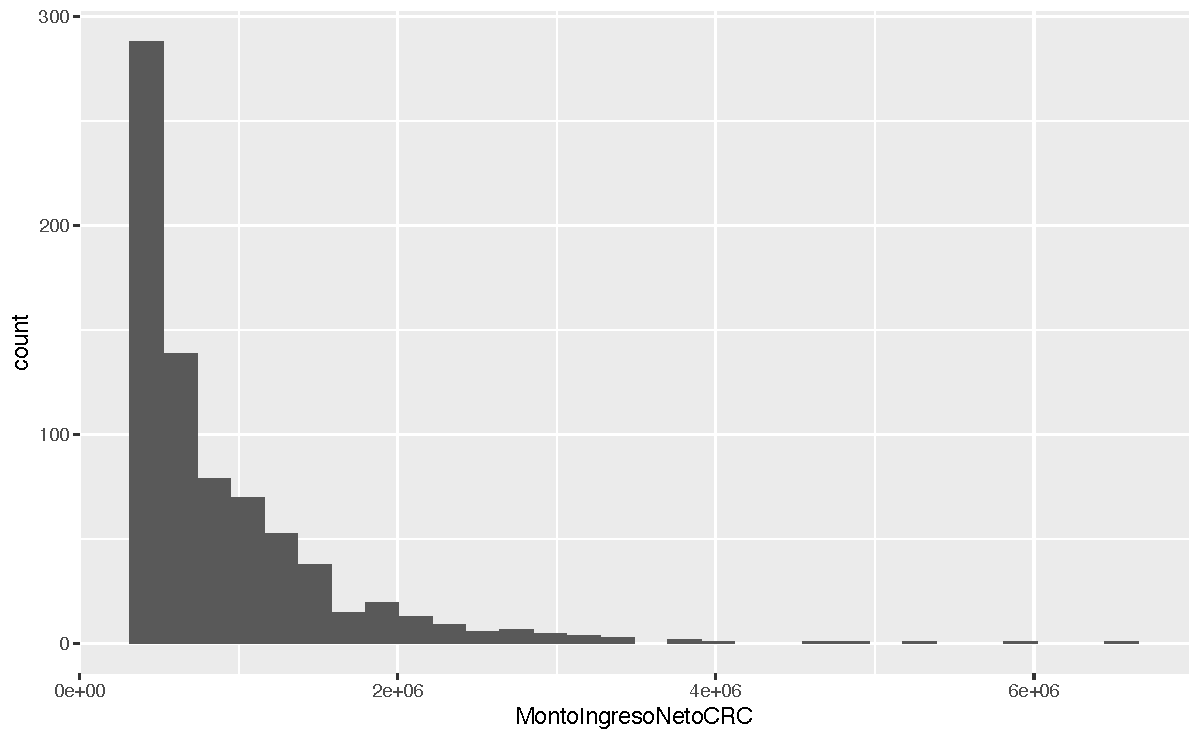
\includegraphics[width=1\linewidth]{Notas-Curso-Basico-R_files/figure-latex/notas-curso-138-1} \end{center}

Dos cosas a considerar del histograma anterior:

\begin{itemize}
\tightlist
\item
  Por defecto, el número de intervalos es de 30. Es posible establecer el número de intervalos (bins), la amplitud del intervalo (binwidth) o fijar los puntos de corte de los intervalos (breaks).
\item
  El eje Y corresponde al número de observaciones (frecuencias absolutas). Si estamos interesados en representar un histogramas de forma que el área del mismo sume 1, entonces tenemos que cambiar la estética de la siguiente forma:
\end{itemize}

\begin{Shaded}
\begin{Highlighting}[]
\FunctionTok{ggplot}\NormalTok{(datos.ingresos, }\FunctionTok{aes}\NormalTok{(}\AttributeTok{x =}\NormalTok{ monto\_ingreso\_neto\_crc)) }\SpecialCharTok{+}
  \FunctionTok{geom\_histogram}\NormalTok{(}\FunctionTok{aes}\NormalTok{(}\AttributeTok{y =}\NormalTok{ ..density..))}
\end{Highlighting}
\end{Shaded}

\begin{center}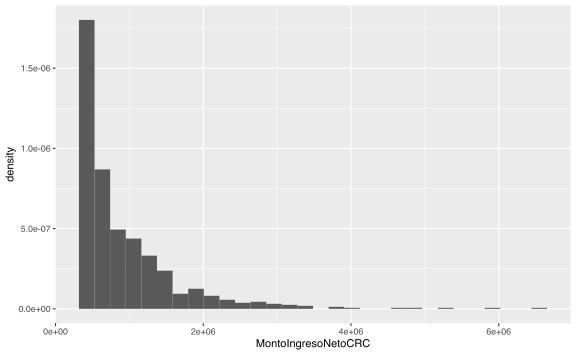
\includegraphics[width=1\linewidth]{Notas-Curso-Basico-R_files/figure-latex/notas-curso-139-1} \end{center}

A partir de esta estructura básica, podemos ir añadiendo elementos para mejorar la presentación.

\begin{Shaded}
\begin{Highlighting}[]
\CommentTok{\# Histograma con 20 intervalos}
\FunctionTok{ggplot}\NormalTok{(datos.ingresos, }\FunctionTok{aes}\NormalTok{(}\AttributeTok{x =}\NormalTok{ monto\_ingreso\_neto\_crc)) }\SpecialCharTok{+}
  \FunctionTok{geom\_histogram}\NormalTok{(}\AttributeTok{bins =} \DecValTok{20}\NormalTok{, }\AttributeTok{color =} \StringTok{"white"}\NormalTok{, }\AttributeTok{fill =} \StringTok{"blue"}\NormalTok{)}
\end{Highlighting}
\end{Shaded}

\begin{center}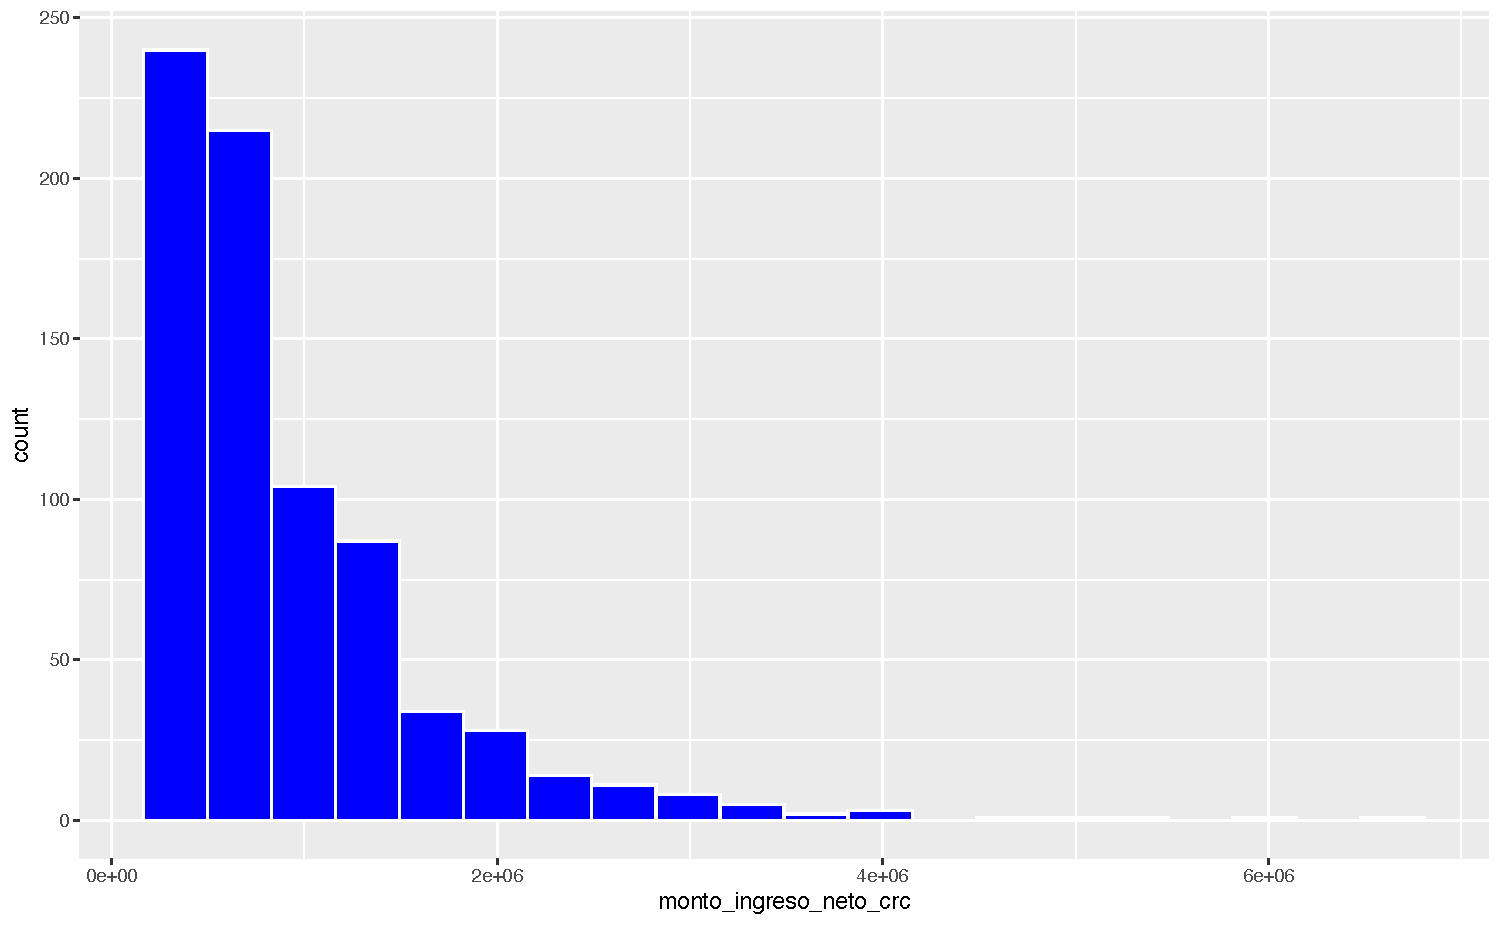
\includegraphics[width=1\linewidth]{Notas-Curso-Basico-R_files/figure-latex/notas-curso-140-1} \end{center}

Ahora vamos a insertar un título al gráfico y también rotularemos los ejes. Para modificar las etiquetas de los ejes se utilizan las funciones xlab() y ylab(). Si, por ejemplo, quisiéramos omitir la etiqueta del eje Y agregamos: ylab(NULL).

También se pueden modificar los límites de los ejes, para esto se utilizan las funciones xlim() y ylim().

\begin{Shaded}
\begin{Highlighting}[]
\FunctionTok{ggplot}\NormalTok{(datos.ingresos, }\FunctionTok{aes}\NormalTok{(}\AttributeTok{x =}\NormalTok{ monto\_ingreso\_neto\_crc)) }\SpecialCharTok{+}
  \FunctionTok{geom\_histogram}\NormalTok{(}\AttributeTok{bins =} \DecValTok{20}\NormalTok{, }\AttributeTok{color =} \StringTok{"white"}\NormalTok{, }\AttributeTok{fill =} \StringTok{"blue"}\NormalTok{) }\SpecialCharTok{+}
  \FunctionTok{ggtitle}\NormalTok{(}\StringTok{"Distribución del ingreso neto "}\NormalTok{) }\SpecialCharTok{+}
  \FunctionTok{xlab}\NormalTok{(}\StringTok{"Salario"}\NormalTok{) }\SpecialCharTok{+}
  \FunctionTok{ylab}\NormalTok{(}\StringTok{"Número de clientes"}\NormalTok{)}
\end{Highlighting}
\end{Shaded}

\begin{center}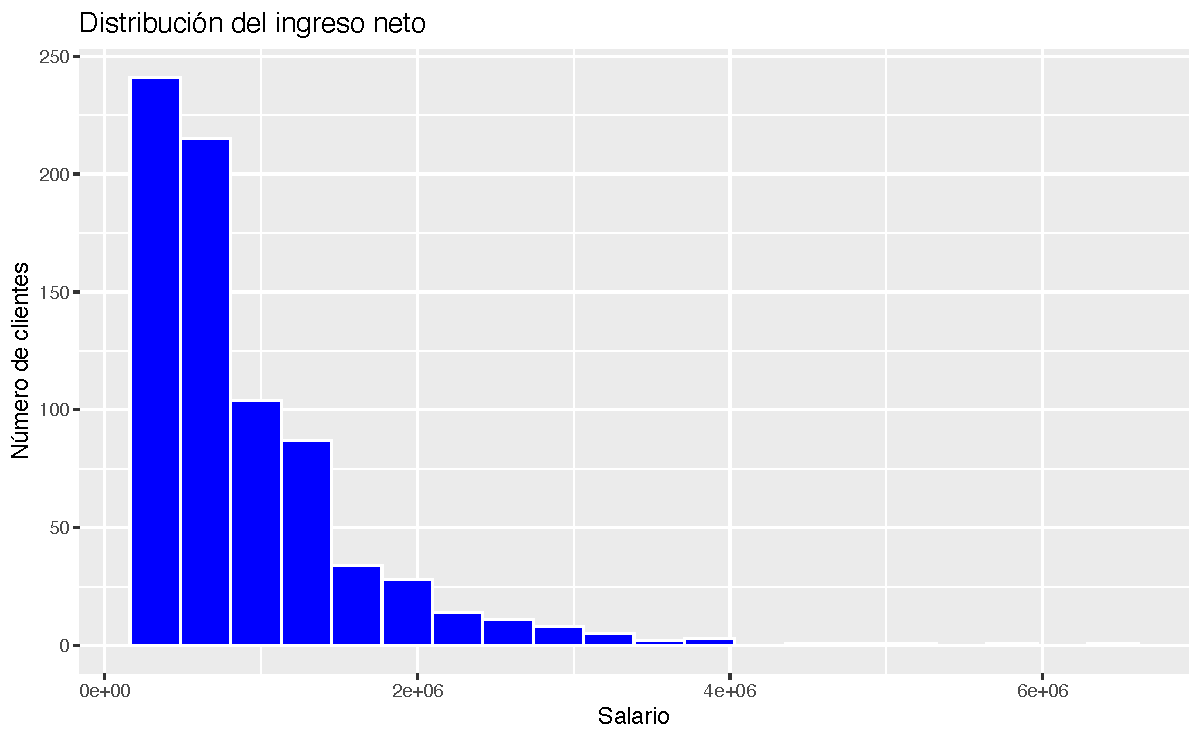
\includegraphics[width=1\linewidth]{Notas-Curso-Basico-R_files/figure-latex/notas-curso-141-1} \end{center}

\begin{Shaded}
\begin{Highlighting}[]
\CommentTok{\# Una alternativa al anterior sería:}

\FunctionTok{ggplot}\NormalTok{(datos.ingresos, }\FunctionTok{aes}\NormalTok{(}\AttributeTok{x =}\NormalTok{ monto\_ingreso\_neto\_crc)) }\SpecialCharTok{+}
  \FunctionTok{geom\_histogram}\NormalTok{(}\AttributeTok{bins =} \DecValTok{20}\NormalTok{, }\AttributeTok{color =} \StringTok{"white"}\NormalTok{, }\AttributeTok{fill =} \StringTok{"blue"}\NormalTok{) }\SpecialCharTok{+}
  \FunctionTok{labs}\NormalTok{(}\AttributeTok{title =} \StringTok{"Distribución del ingreso neto"}\NormalTok{,}
    \AttributeTok{x =} \StringTok{"Ingreso"}\NormalTok{,}
    \AttributeTok{y =} \StringTok{"Número de clientes"}\NormalTok{) }\SpecialCharTok{+}
  \FunctionTok{ylim}\NormalTok{(}\FunctionTok{c}\NormalTok{(}\DecValTok{0}\NormalTok{, }\DecValTok{250}\NormalTok{))}
\end{Highlighting}
\end{Shaded}

\begin{center}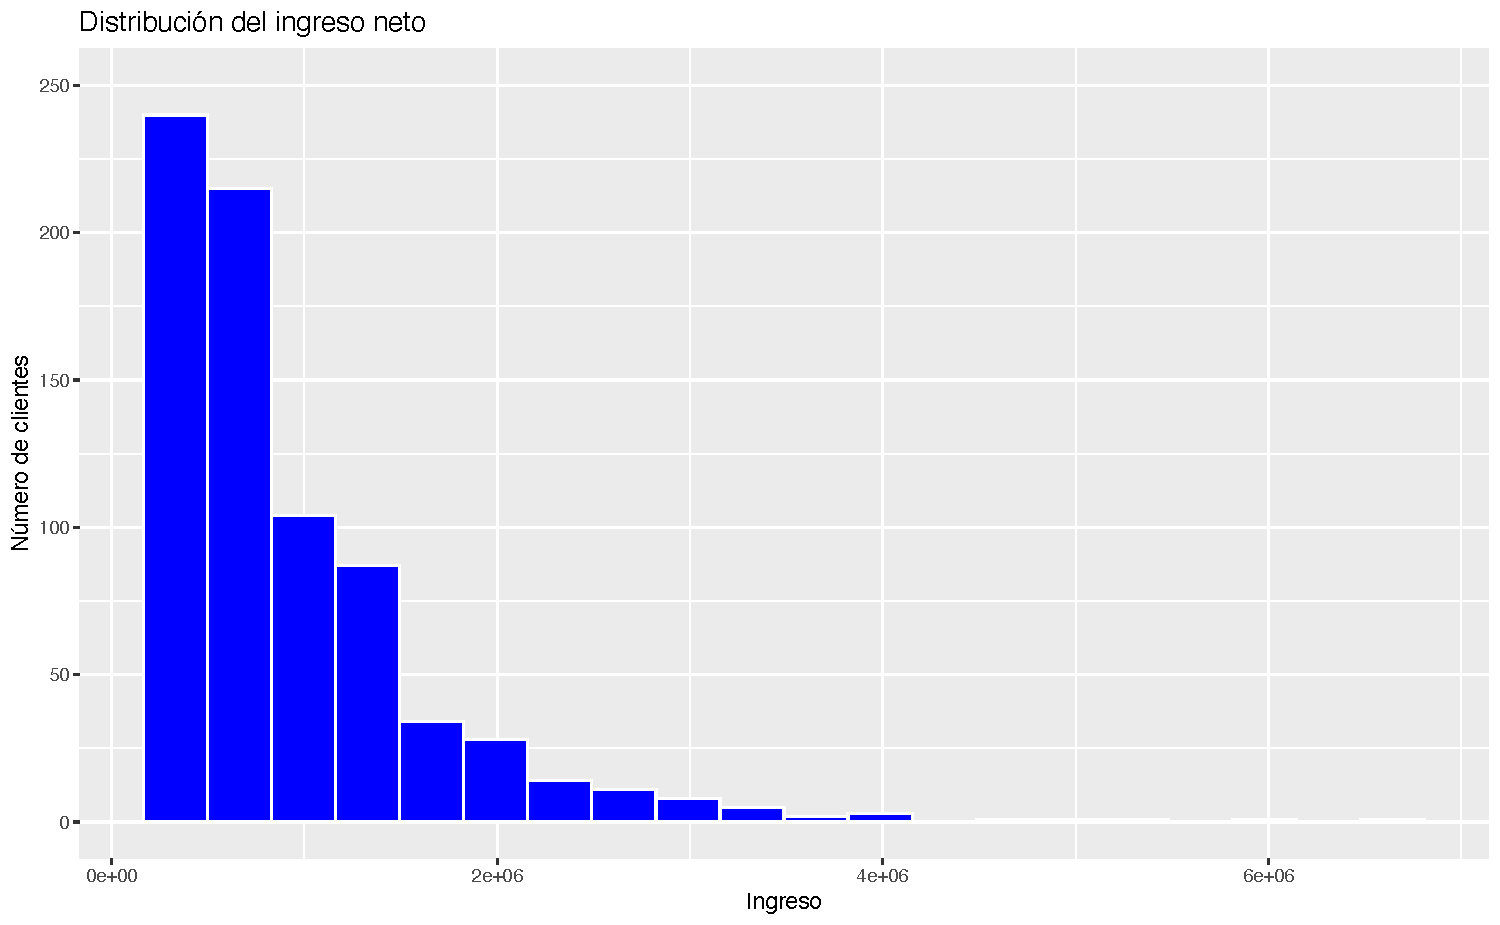
\includegraphics[width=1\linewidth]{Notas-Curso-Basico-R_files/figure-latex/notas-curso-142-1} \end{center}

Para tratar de observar las diferencias en la distribución del salario según distintos grupo, por ejemplo, el género podemos:

Visualizar cada subconjunto de datos (ingreso neto para asalariados e independientes ) en distintos paneles. Para ello, utilizamos el elemento facet.

\begin{Shaded}
\begin{Highlighting}[]
\FunctionTok{ggplot}\NormalTok{(datos.ingresos, }\FunctionTok{aes}\NormalTok{(}\AttributeTok{x =}\NormalTok{ monto\_ingreso\_neto\_crc)) }\SpecialCharTok{+}
  \FunctionTok{geom\_histogram}\NormalTok{(}\AttributeTok{bins =} \DecValTok{20}\NormalTok{, }\AttributeTok{color =} \StringTok{"white"}\NormalTok{, }\AttributeTok{fill =} \StringTok{"blue"}\NormalTok{) }\SpecialCharTok{+}
  \FunctionTok{facet\_grid}\NormalTok{(tipo\_empleado }\SpecialCharTok{\textasciitilde{}}\NormalTok{ .)}
\end{Highlighting}
\end{Shaded}

\begin{center}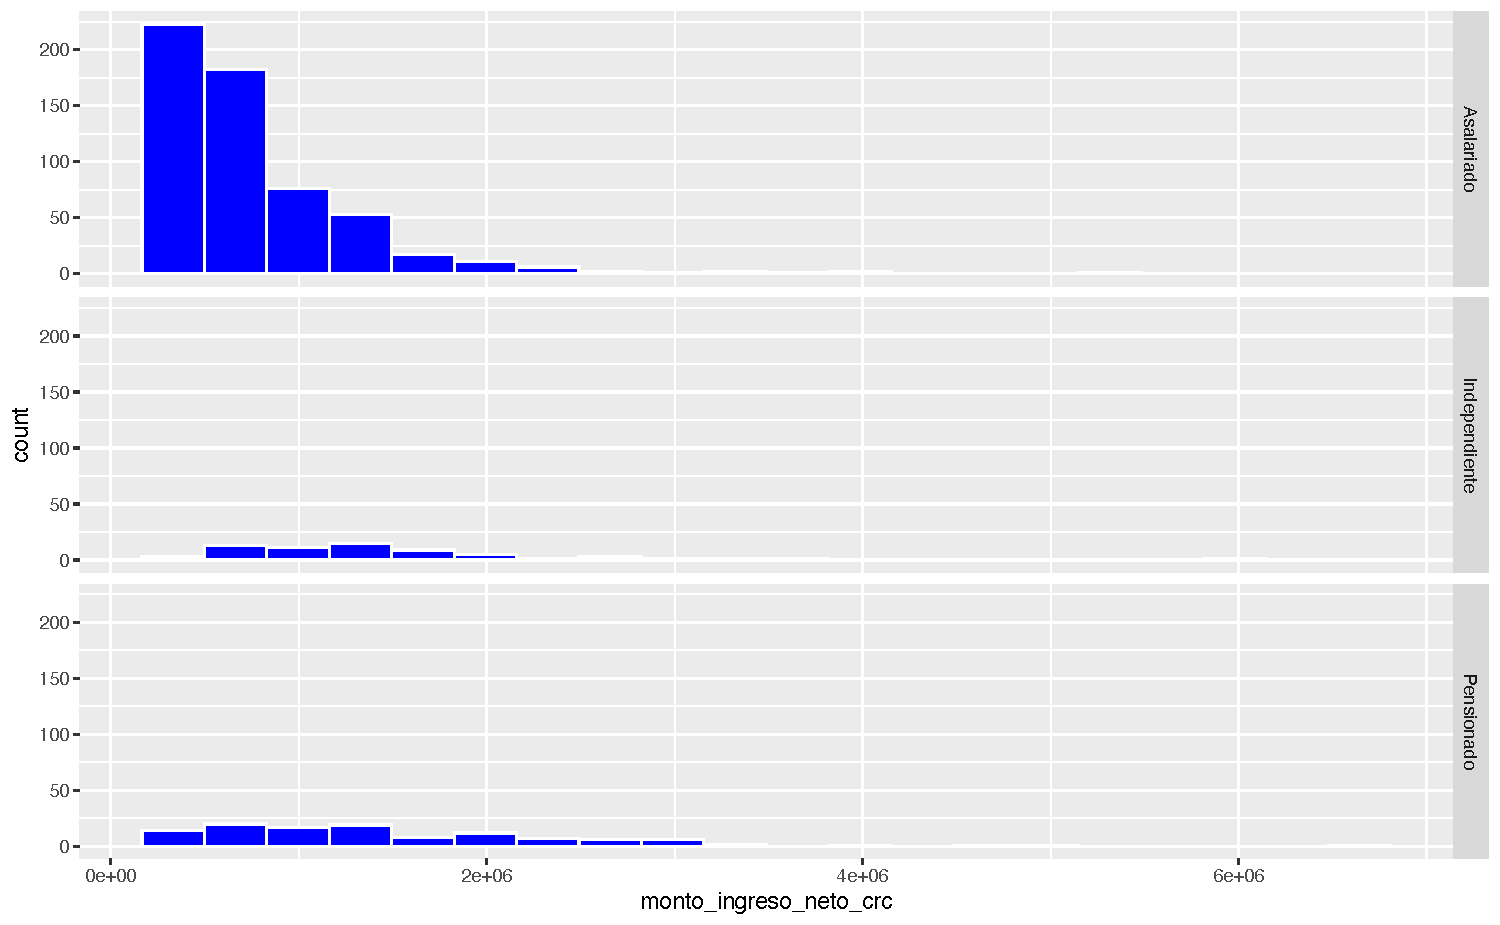
\includegraphics[width=1\linewidth]{Notas-Curso-Basico-R_files/figure-latex/notas-curso-143-1} \end{center}

\begin{Shaded}
\begin{Highlighting}[]
\FunctionTok{ggplot}\NormalTok{(datos.ingresos, }\FunctionTok{aes}\NormalTok{(}\AttributeTok{x =}\NormalTok{ monto\_ingreso\_neto\_crc)) }\SpecialCharTok{+}
  \FunctionTok{geom\_histogram}\NormalTok{(}\AttributeTok{bins =} \DecValTok{20}\NormalTok{, }\AttributeTok{color =} \StringTok{"white"}\NormalTok{, }\AttributeTok{fill =} \StringTok{"blue"}\NormalTok{) }\SpecialCharTok{+}
  \FunctionTok{facet\_wrap}\NormalTok{(}\SpecialCharTok{\textasciitilde{}}\NormalTok{tipo\_empleado)}
\end{Highlighting}
\end{Shaded}

\begin{center}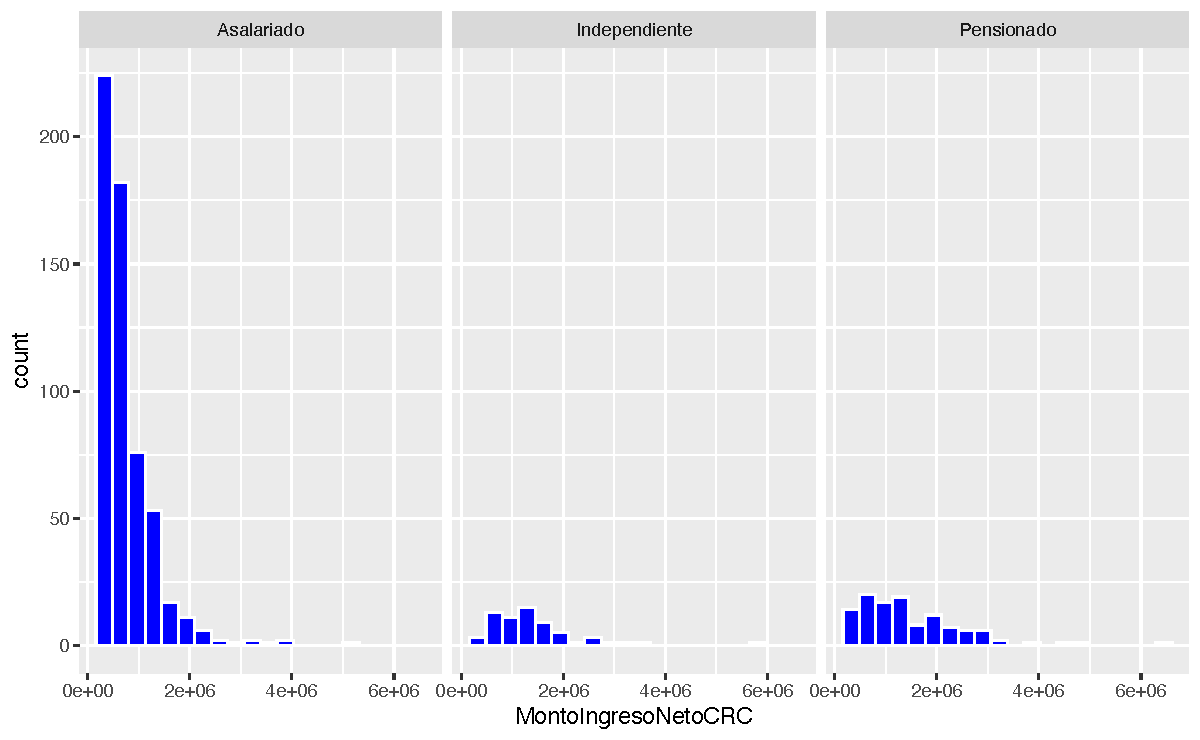
\includegraphics[width=1\linewidth]{Notas-Curso-Basico-R_files/figure-latex/notas-curso-144-1} \end{center}

Hacemos el histograma pero usamos el tipo\_empleado de cliente para colorear las partes que de cada intervalo corresponden a asalariados, independientes y a pensionados.

\begin{Shaded}
\begin{Highlighting}[]
\FunctionTok{ggplot}\NormalTok{(datos.ingresos, }\FunctionTok{aes}\NormalTok{(}\AttributeTok{x =}\NormalTok{ monto\_ingreso\_neto\_crc, }\AttributeTok{fill =}\NormalTok{ tipo\_empleado)) }\SpecialCharTok{+}
  \FunctionTok{geom\_histogram}\NormalTok{(}\AttributeTok{bins =} \DecValTok{20}\NormalTok{) }\SpecialCharTok{+}
  \FunctionTok{ylim}\NormalTok{(}\FunctionTok{c}\NormalTok{(}\DecValTok{0}\NormalTok{, }\DecValTok{250}\NormalTok{))}
\end{Highlighting}
\end{Shaded}

\begin{center}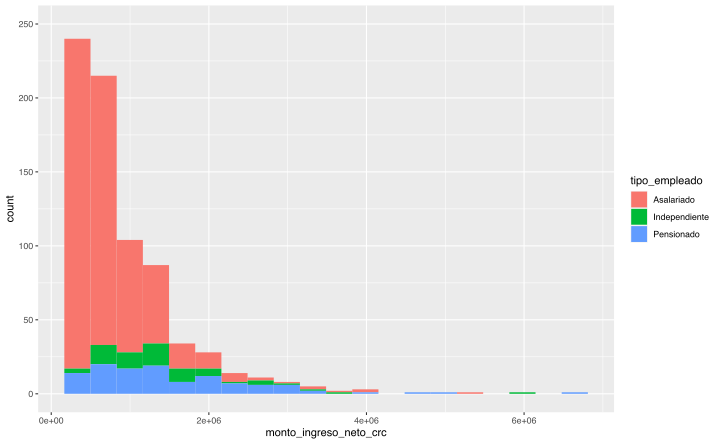
\includegraphics[width=1\linewidth]{Notas-Curso-Basico-R_files/figure-latex/notas-curso-145-1} \end{center}

\begin{Shaded}
\begin{Highlighting}[]
\FunctionTok{ggplot}\NormalTok{(datos.ingresos, }\FunctionTok{aes}\NormalTok{(}\AttributeTok{x =}\NormalTok{ monto\_ingreso\_neto\_crc)) }\SpecialCharTok{+}
  \FunctionTok{geom\_histogram}\NormalTok{(}\AttributeTok{bins =} \DecValTok{10}\NormalTok{, }\FunctionTok{aes}\NormalTok{(}\AttributeTok{fill =}\NormalTok{ tipo\_empleado), }\AttributeTok{position =} \StringTok{"fill"}\NormalTok{, }\AttributeTok{alpha =} \FloatTok{0.4}\NormalTok{) }\SpecialCharTok{+}
  \FunctionTok{labs}\NormalTok{(}\AttributeTok{x =} \StringTok{"Ingreso neto"}\NormalTok{, }\AttributeTok{y =} \StringTok{"Clientes"}\NormalTok{, }\AttributeTok{fill =} \StringTok{"tipo\_empleado"}\NormalTok{) }\SpecialCharTok{+}  \CommentTok{\# títulos de ejes y leyenda}
  \FunctionTok{scale\_fill\_discrete}\NormalTok{(}\AttributeTok{labels =} \FunctionTok{c}\NormalTok{(}\StringTok{"Asalariado"}\NormalTok{, }\StringTok{"Independiente"}\NormalTok{, }\StringTok{"Pensionado"}\NormalTok{))     }\CommentTok{\# títulos claves leyenda}
\end{Highlighting}
\end{Shaded}

\begin{center}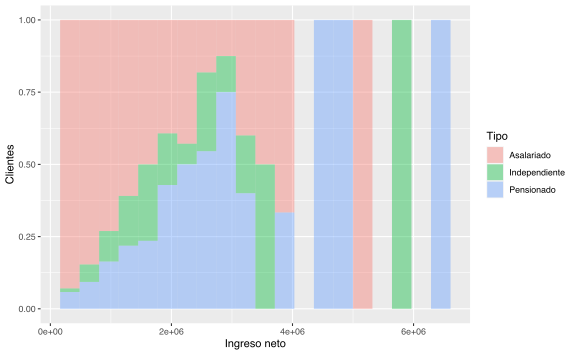
\includegraphics[width=1\linewidth]{Notas-Curso-Basico-R_files/figure-latex/notas-curso-146-1} \end{center}

\hypertarget{gruxe1ficos-de-dispersiuxf3n}{%
\section{\texorpdfstring{\textbf{Gráficos de dispersión}}{Gráficos de dispersión}}\label{gruxe1ficos-de-dispersiuxf3n}}

\begin{Shaded}
\begin{Highlighting}[]
\CommentTok{\# Opción 1}
\FunctionTok{ggplot}\NormalTok{(datos.ingresos, }\FunctionTok{aes}\NormalTok{(monto\_ingreso\_bruto\_crc, monto\_ingreso\_neto\_crc, }\AttributeTok{color =}\NormalTok{ tipo\_empleado)) }\SpecialCharTok{+}
  \FunctionTok{geom\_point}\NormalTok{() }\SpecialCharTok{+}
  \FunctionTok{labs}\NormalTok{(}\AttributeTok{title =} \StringTok{"Gráfico de dispersión"}\NormalTok{,}
    \AttributeTok{subtitle =} \StringTok{"ScatterPlot"}\NormalTok{,}
    \AttributeTok{caption =} \StringTok{"Fuente: DGR"}\NormalTok{,}
    \AttributeTok{x =} \StringTok{"Ingreso bruto"}\NormalTok{,}
    \AttributeTok{y =} \StringTok{"Ingreso neto"}\NormalTok{) }\SpecialCharTok{+}
  \FunctionTok{scale\_color\_discrete}\NormalTok{(}\AttributeTok{name =} \StringTok{"tipo\_empleado"}\NormalTok{, }\AttributeTok{labels =} \FunctionTok{c}\NormalTok{(}\StringTok{"Asalariado"}\NormalTok{, }\StringTok{"Independiente"}\NormalTok{, }\StringTok{"Pensionado"}\NormalTok{))}
\end{Highlighting}
\end{Shaded}

\begin{center}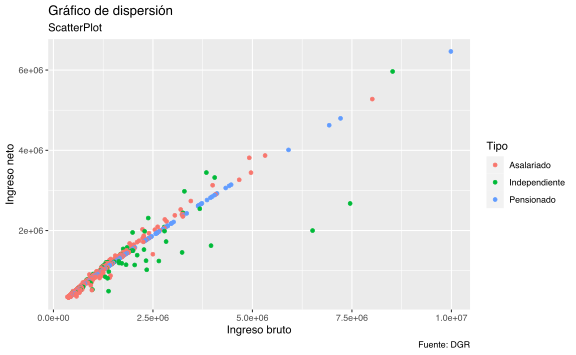
\includegraphics[width=1\linewidth]{Notas-Curso-Basico-R_files/figure-latex/notas-curso-147-1} \end{center}

\begin{Shaded}
\begin{Highlighting}[]
\FunctionTok{ggplot}\NormalTok{(datos.ingresos, }\FunctionTok{aes}\NormalTok{(monto\_ingreso\_bruto\_crc, monto\_ingreso\_neto\_crc, }\AttributeTok{color =}\NormalTok{ tipo\_empleado)) }\SpecialCharTok{+}
  \FunctionTok{geom\_point}\NormalTok{() }\SpecialCharTok{+}
  \FunctionTok{geom\_smooth}\NormalTok{(}\AttributeTok{method =} \StringTok{"lm"}\NormalTok{, }\AttributeTok{se =} \ConstantTok{FALSE}\NormalTok{) }\SpecialCharTok{+}
  \FunctionTok{labs}\NormalTok{(}\AttributeTok{title =} \StringTok{"Gráfico de dispersión"}\NormalTok{,}
    \AttributeTok{subtitle =} \StringTok{"ScatterPlot"}\NormalTok{,}
    \AttributeTok{caption =} \StringTok{"Fuente: DGR"}\NormalTok{,}
    \AttributeTok{x =} \StringTok{"Ingreso bruto"}\NormalTok{,}
    \AttributeTok{y =} \StringTok{"Ingreso neto"}\NormalTok{) }\SpecialCharTok{+}
  \FunctionTok{scale\_color\_discrete}\NormalTok{(}\AttributeTok{name =} \StringTok{"tipo\_empleado"}\NormalTok{, }\AttributeTok{labels =} \FunctionTok{c}\NormalTok{(}\StringTok{"Asalariado"}\NormalTok{, }\StringTok{"Independiente"}\NormalTok{, }\StringTok{"Pensionado"}\NormalTok{))}
\end{Highlighting}
\end{Shaded}

\begin{center}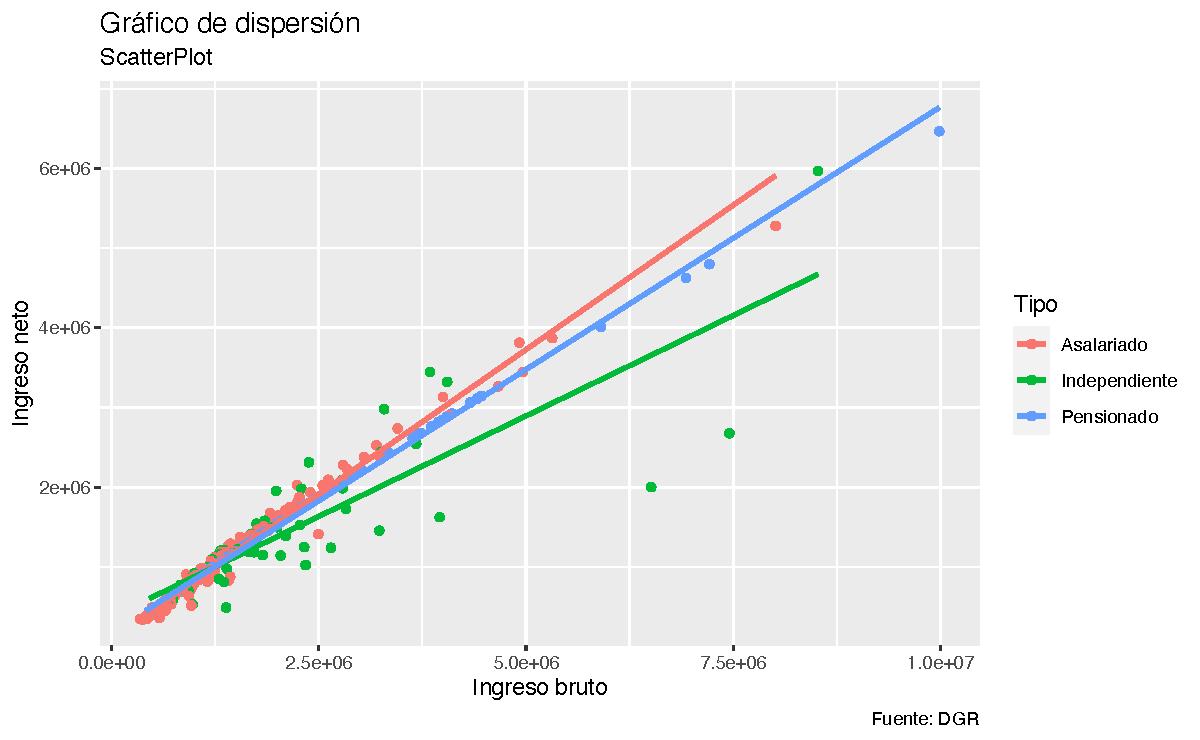
\includegraphics[width=1\linewidth]{Notas-Curso-Basico-R_files/figure-latex/notas-curso-148-1} \end{center}

\begin{Shaded}
\begin{Highlighting}[]
\FunctionTok{ggplot}\NormalTok{(datos.ingresos, }\FunctionTok{aes}\NormalTok{(monto\_ingreso\_bruto\_crc, monto\_ingreso\_neto\_crc, }\AttributeTok{color =}\NormalTok{ tipo\_empleado)) }\SpecialCharTok{+}
  \FunctionTok{geom\_point}\NormalTok{() }\SpecialCharTok{+}
  \FunctionTok{geom\_smooth}\NormalTok{(}\AttributeTok{method =} \StringTok{"lm"}\NormalTok{) }\SpecialCharTok{+}
  \FunctionTok{labs}\NormalTok{(}\AttributeTok{title =} \StringTok{"Gráfico de dispersión"}\NormalTok{,}
    \AttributeTok{subtitle =} \StringTok{"ScatterPlot"}\NormalTok{,}
    \AttributeTok{caption =} \StringTok{"Fuente: DGR"}\NormalTok{,}
    \AttributeTok{x =} \StringTok{"Ingreso bruto"}\NormalTok{,}
    \AttributeTok{y =} \StringTok{"Ingreso neto"}\NormalTok{) }\SpecialCharTok{+}
  \FunctionTok{scale\_color\_discrete}\NormalTok{(}\AttributeTok{name =} \StringTok{"tipo\_empleado"}\NormalTok{, }\AttributeTok{labels =} \FunctionTok{c}\NormalTok{(}\StringTok{"Asalariado"}\NormalTok{, }\StringTok{"Independiente"}\NormalTok{, }\StringTok{"Pensionado"}\NormalTok{))}
\end{Highlighting}
\end{Shaded}

\begin{center}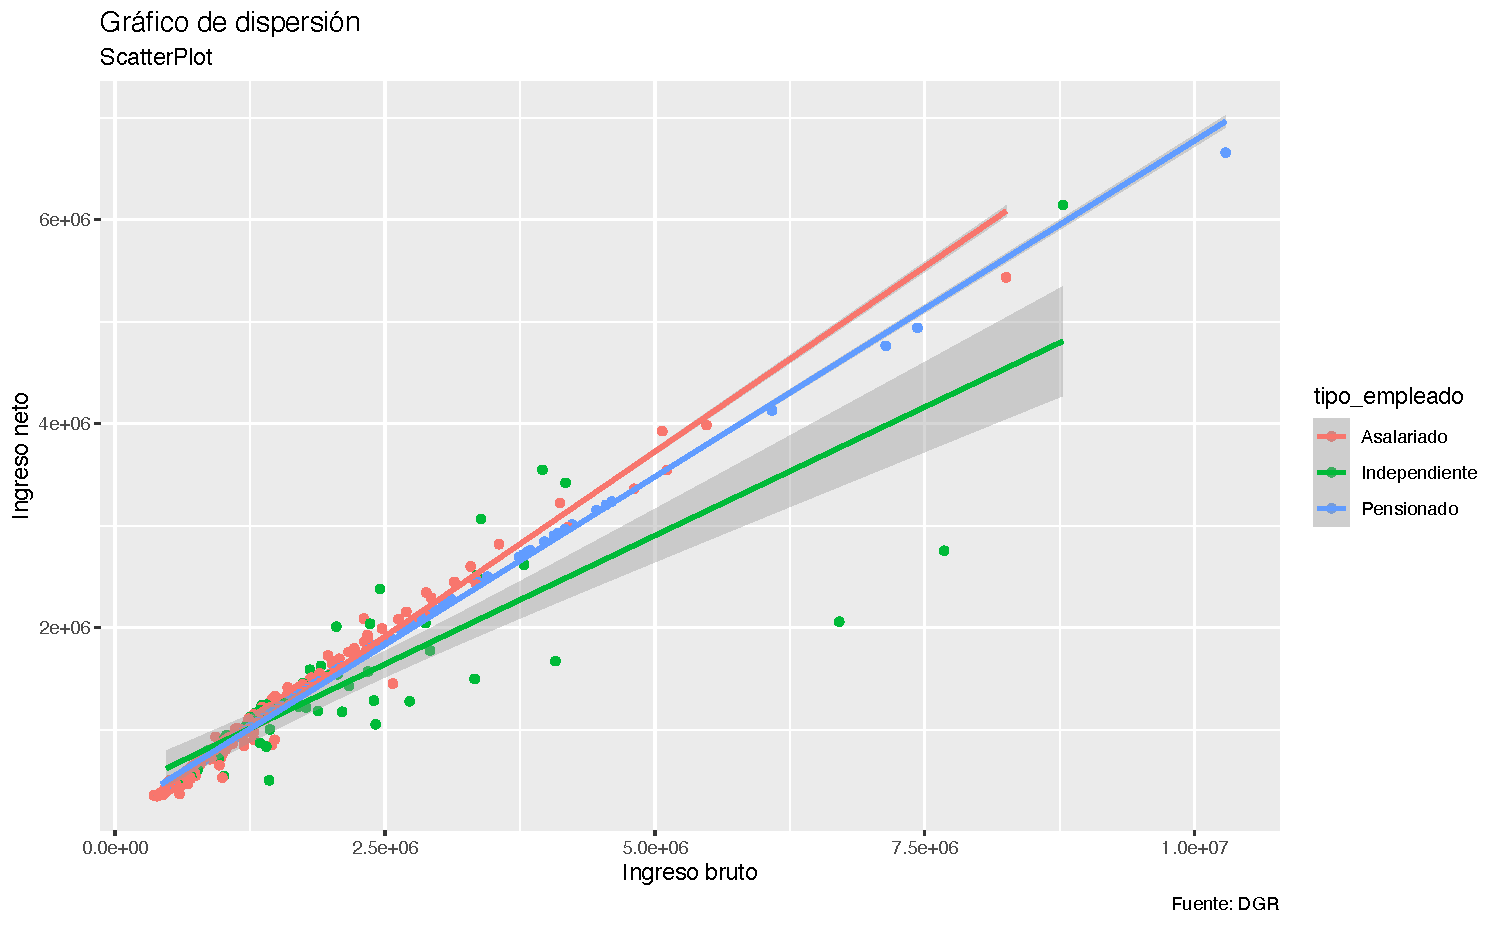
\includegraphics[width=1\linewidth]{Notas-Curso-Basico-R_files/figure-latex/notas-curso-149-1} \end{center}

\hypertarget{gruxe1ficos-de-cajas}{%
\section{\texorpdfstring{\textbf{Gráficos de cajas}}{Gráficos de cajas}}\label{gruxe1ficos-de-cajas}}

\begin{Shaded}
\begin{Highlighting}[]
\FunctionTok{ggplot}\NormalTok{(datos.ingresos, }\FunctionTok{aes}\NormalTok{(}\AttributeTok{x =}\NormalTok{ tipo\_empleado, }\AttributeTok{y =}\NormalTok{ monto\_ingreso\_neto\_crc)) }\SpecialCharTok{+}
  \FunctionTok{geom\_boxplot}\NormalTok{()}
\end{Highlighting}
\end{Shaded}

\begin{center}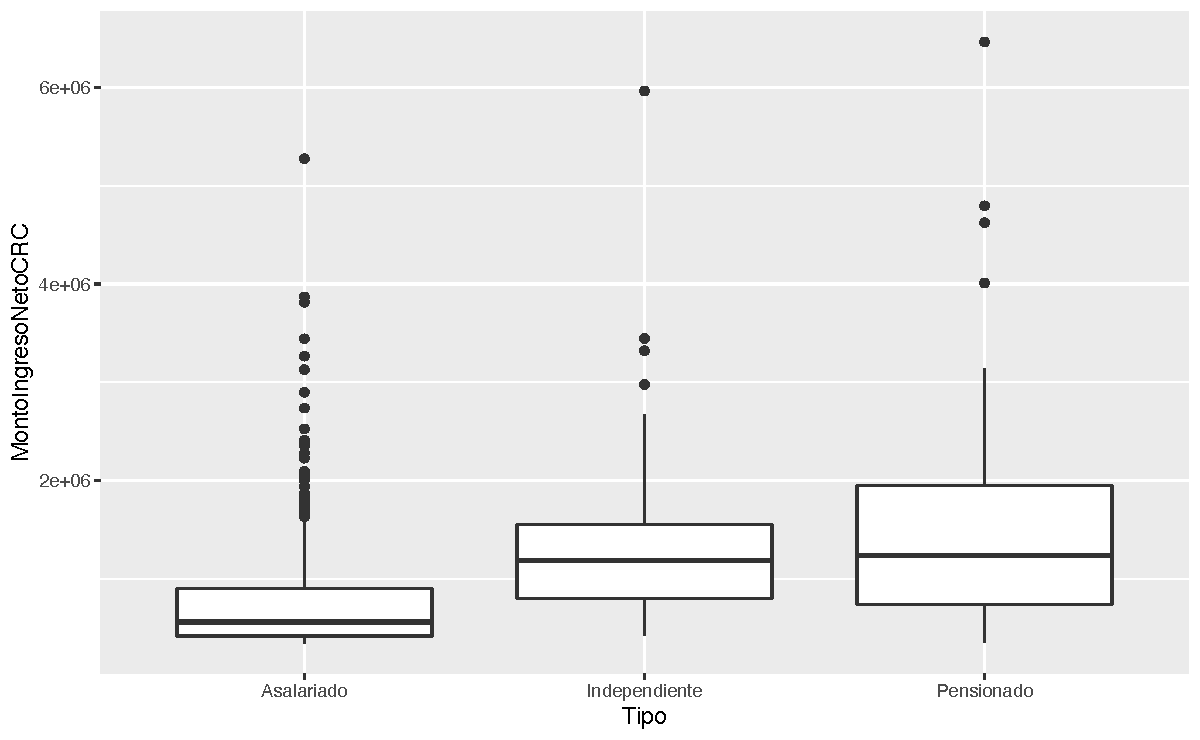
\includegraphics[width=1\linewidth]{Notas-Curso-Basico-R_files/figure-latex/notas-curso-150-1} \end{center}

\begin{Shaded}
\begin{Highlighting}[]
\CommentTok{\# Diagrama de caja con color de relleno}
\FunctionTok{ggplot}\NormalTok{(datos.ingresos, }\FunctionTok{aes}\NormalTok{(}\AttributeTok{x =}\NormalTok{ tipo\_empleado, }\AttributeTok{y =}\NormalTok{ monto\_ingreso\_neto\_crc, }\AttributeTok{fill =}\NormalTok{ tipo\_empleado))  }\SpecialCharTok{+}
  \FunctionTok{geom\_boxplot}\NormalTok{() }\SpecialCharTok{+}
  \FunctionTok{labs}\NormalTok{(}\AttributeTok{x =} \StringTok{"Tipo de cliente"}\NormalTok{, }\AttributeTok{y =} \StringTok{"Ingreso"}\NormalTok{, }\AttributeTok{fill =} \StringTok{"tipo\_empleado"}\NormalTok{) }\SpecialCharTok{+}   \CommentTok{\# titulo ejes y leyenda}
  \FunctionTok{scale\_x\_discrete}\NormalTok{(}\AttributeTok{labels =} \FunctionTok{c}\NormalTok{(}\StringTok{"Asalariado"}\NormalTok{, }\StringTok{"Independiente"}\NormalTok{, }\StringTok{"Pensionado"}\NormalTok{)) }\SpecialCharTok{+}   \CommentTok{\# etiquetas del eje x}
  \FunctionTok{scale\_fill\_discrete}\NormalTok{(}\AttributeTok{labels =} \FunctionTok{c}\NormalTok{(}\StringTok{"Asalariado"}\NormalTok{, }\StringTok{"Independiente"}\NormalTok{, }\StringTok{"Pensionado"}\NormalTok{))  }\CommentTok{\# etiquetas claves leyenda}
\end{Highlighting}
\end{Shaded}

\begin{center}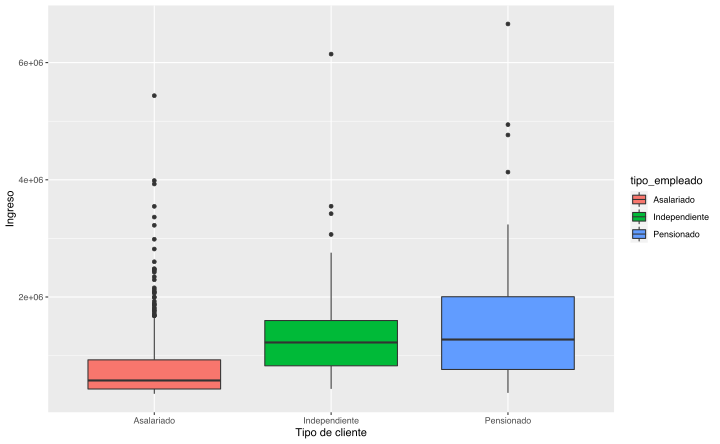
\includegraphics[width=1\linewidth]{Notas-Curso-Basico-R_files/figure-latex/notas-curso-151-1} \end{center}

\begin{Shaded}
\begin{Highlighting}[]
\CommentTok{\# Diagrama de caja sin leyenda por considerar redundante la información}

\FunctionTok{ggplot}\NormalTok{(datos.ingresos, }\FunctionTok{aes}\NormalTok{(}\AttributeTok{x =}\NormalTok{ tipo\_empleado, }\AttributeTok{y =}\NormalTok{ monto\_ingreso\_neto\_crc, }\AttributeTok{fill =}\NormalTok{ tipo\_empleado))   }\SpecialCharTok{+}
  \FunctionTok{geom\_boxplot}\NormalTok{(}\AttributeTok{outlier.colour =} \StringTok{"blue"}\NormalTok{) }\SpecialCharTok{+}             \CommentTok{\# color de los outliers}
  \FunctionTok{labs}\NormalTok{(}\AttributeTok{x =} \StringTok{"Tipo cliente"}\NormalTok{, }\AttributeTok{y =} \StringTok{"Ingreso"}\NormalTok{) }\SpecialCharTok{+}
  \FunctionTok{scale\_x\_discrete}\NormalTok{(}\AttributeTok{labels =} \FunctionTok{c}\NormalTok{(}\StringTok{"Asalariado"}\NormalTok{, }\StringTok{"Independiente"}\NormalTok{, }\StringTok{"Pensionado"}\NormalTok{)) }\SpecialCharTok{+}
  \FunctionTok{guides}\NormalTok{(}\AttributeTok{fill =} \ConstantTok{FALSE}\NormalTok{)}
\end{Highlighting}
\end{Shaded}

\begin{center}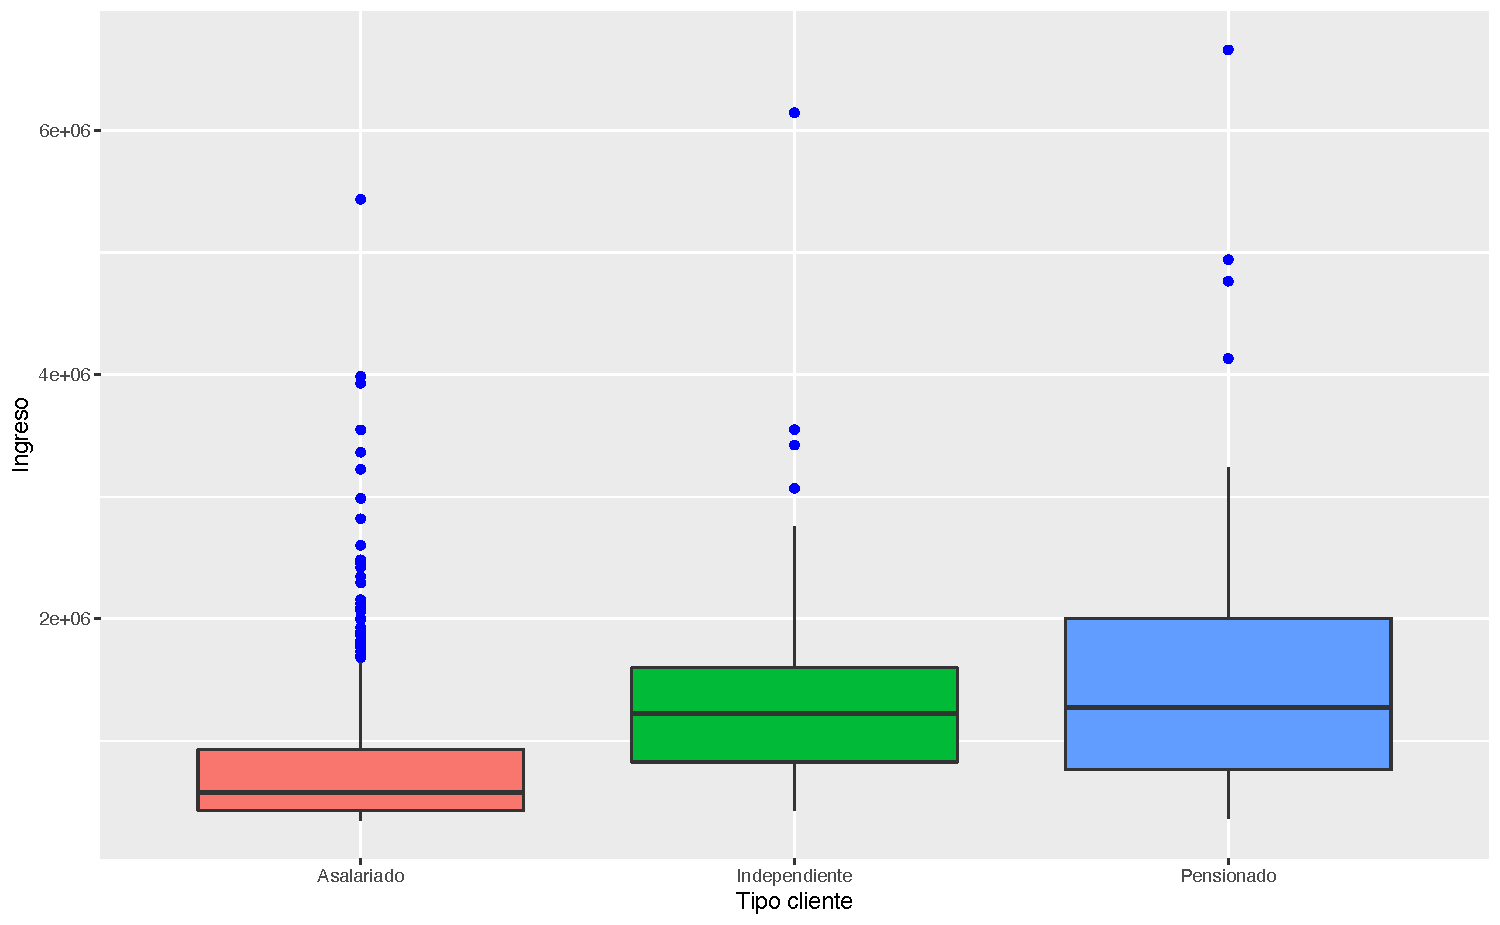
\includegraphics[width=1\linewidth]{Notas-Curso-Basico-R_files/figure-latex/notas-curso-152-1} \end{center}

\begin{Shaded}
\begin{Highlighting}[]
\CommentTok{\# eliminamos la leyenda}
\end{Highlighting}
\end{Shaded}

\begin{Shaded}
\begin{Highlighting}[]
\FunctionTok{ggplot}\NormalTok{(datos.ingresos, }\FunctionTok{aes}\NormalTok{(}\AttributeTok{x =}\NormalTok{ tipo\_empleado, }\AttributeTok{y =}\NormalTok{ monto\_ingreso\_neto\_crc, }\AttributeTok{fill =}\NormalTok{ tipo\_empleado))  }\SpecialCharTok{+}
  \FunctionTok{geom\_boxplot}\NormalTok{(}\AttributeTok{outlier.colour =} \StringTok{"blue"}\NormalTok{) }\SpecialCharTok{+}
  \FunctionTok{labs}\NormalTok{(}\AttributeTok{x =} \StringTok{"Tipo cliente"}\NormalTok{, }\AttributeTok{y =} \StringTok{"Ingreso"}\NormalTok{) }\SpecialCharTok{+}
  \FunctionTok{scale\_x\_discrete}\NormalTok{(}\AttributeTok{labels =} \FunctionTok{c}\NormalTok{(}\StringTok{"Asalariado"}\NormalTok{, }\StringTok{"Independiente"}\NormalTok{, }\StringTok{"Pensionado"}\NormalTok{)) }\SpecialCharTok{+}
  \FunctionTok{guides}\NormalTok{(}\AttributeTok{fill =} \ConstantTok{FALSE}\NormalTok{) }\SpecialCharTok{+}
  \FunctionTok{coord\_flip}\NormalTok{()                       }\CommentTok{\# cambio dirección de las cajas}
\end{Highlighting}
\end{Shaded}

\begin{center}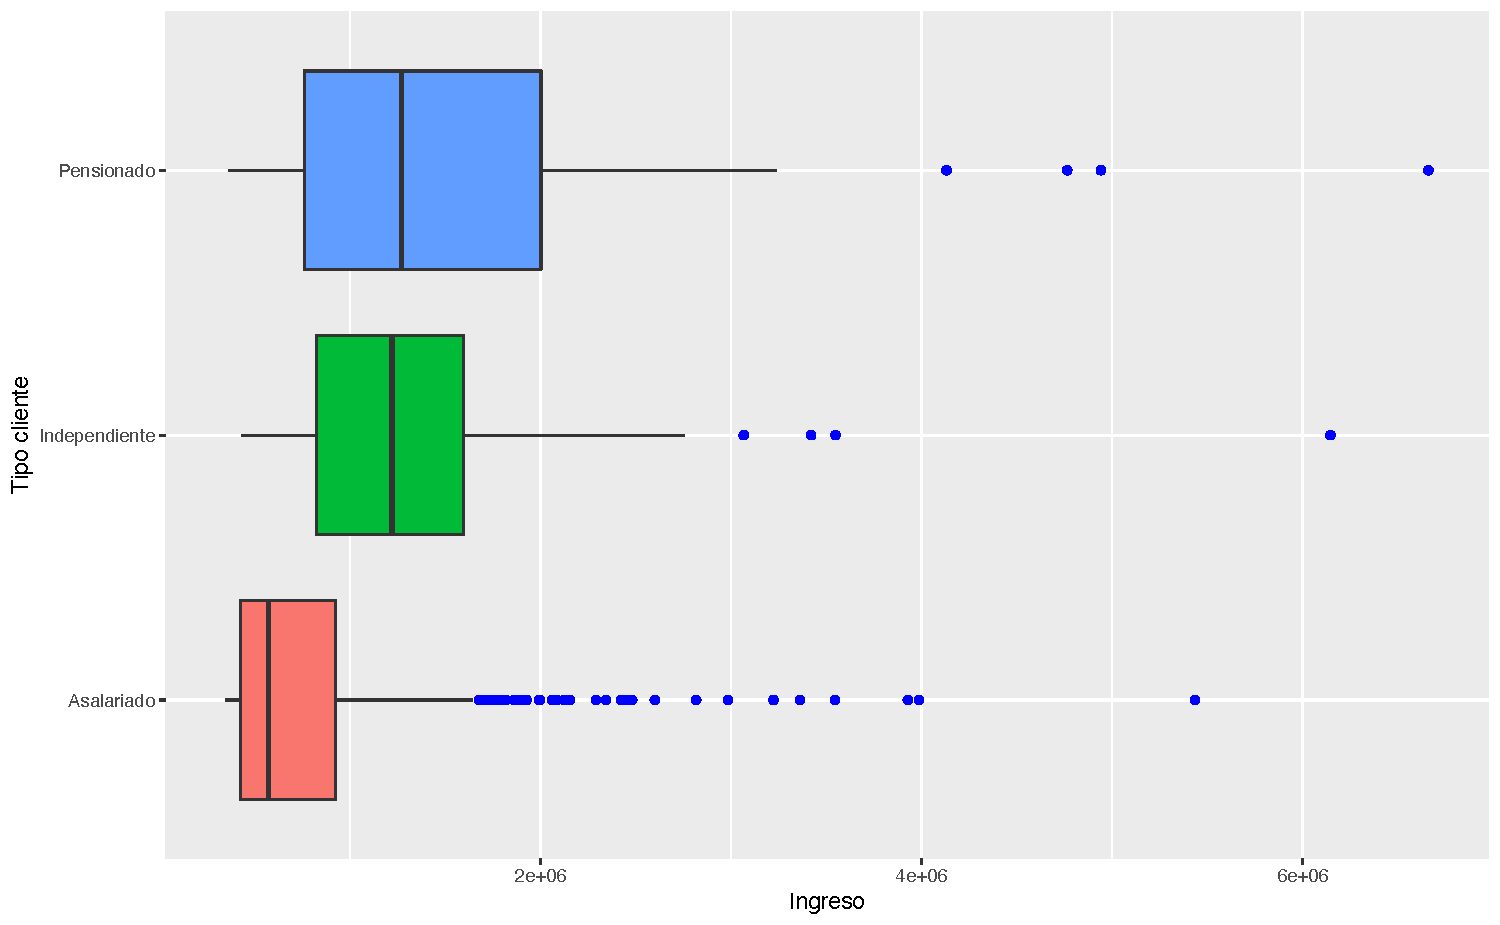
\includegraphics[width=1\linewidth]{Notas-Curso-Basico-R_files/figure-latex/notas-curso-153-1} \end{center}

Puede resultar interesante localizar la media de cada grupo en los diagramas de caja. Para ello, hacemos uso del elemento stat (transformación estadística). Se puede añadir stat, básicamente, de dos formas:

\begin{enumerate}
\def\labelenumi{\arabic{enumi}.}
\tightlist
\item
  Añadir directamente una función stat\_() y de esa forma anular su valor por defecto en la geometría.
\item
  Añadir una función geom\_() e introducir el elemento stat para anular el valor por defecto.
\end{enumerate}

Veamos las dos formas comentadas de añadir.

\begin{Shaded}
\begin{Highlighting}[]
\CommentTok{\# Añadimos la media utilizando la función geom\_() y modificando el elemento stat}
\FunctionTok{ggplot}\NormalTok{(datos.ingresos, }\FunctionTok{aes}\NormalTok{(}\AttributeTok{x =}\NormalTok{ tipo\_empleado, }\AttributeTok{y =}\NormalTok{ monto\_ingreso\_neto\_crc, }\AttributeTok{fill =}\NormalTok{ tipo\_empleado)) }\SpecialCharTok{+}
  \FunctionTok{geom\_boxplot}\NormalTok{(}\AttributeTok{alpha =} \FloatTok{0.3}\NormalTok{, }\AttributeTok{outlier.colour =} \StringTok{"blue"}\NormalTok{) }\SpecialCharTok{+}
  \FunctionTok{labs}\NormalTok{(}\AttributeTok{x =} \StringTok{"Género"}\NormalTok{, }\AttributeTok{y =} \StringTok{"Salario"}\NormalTok{) }\SpecialCharTok{+}
  \FunctionTok{scale\_x\_discrete}\NormalTok{(}\AttributeTok{labels =} \FunctionTok{c}\NormalTok{(}\StringTok{"Asalariado"}\NormalTok{, }\StringTok{"Independiente"}\NormalTok{, }\StringTok{"Pensionado"}\NormalTok{)) }\SpecialCharTok{+}
  \FunctionTok{guides}\NormalTok{(}\AttributeTok{fill =} \ConstantTok{FALSE}\NormalTok{) }\SpecialCharTok{+}
  \FunctionTok{coord\_flip}\NormalTok{() }\SpecialCharTok{+}
  \FunctionTok{geom\_point}\NormalTok{(}\AttributeTok{stat =} \StringTok{"summary"}\NormalTok{, }\AttributeTok{fun.y =}\NormalTok{ mean, }\AttributeTok{shape =} \DecValTok{16}\NormalTok{, }\AttributeTok{size =} \DecValTok{2}\NormalTok{, }\AttributeTok{color =} \StringTok{"red"}\NormalTok{)}
\end{Highlighting}
\end{Shaded}

\begin{center}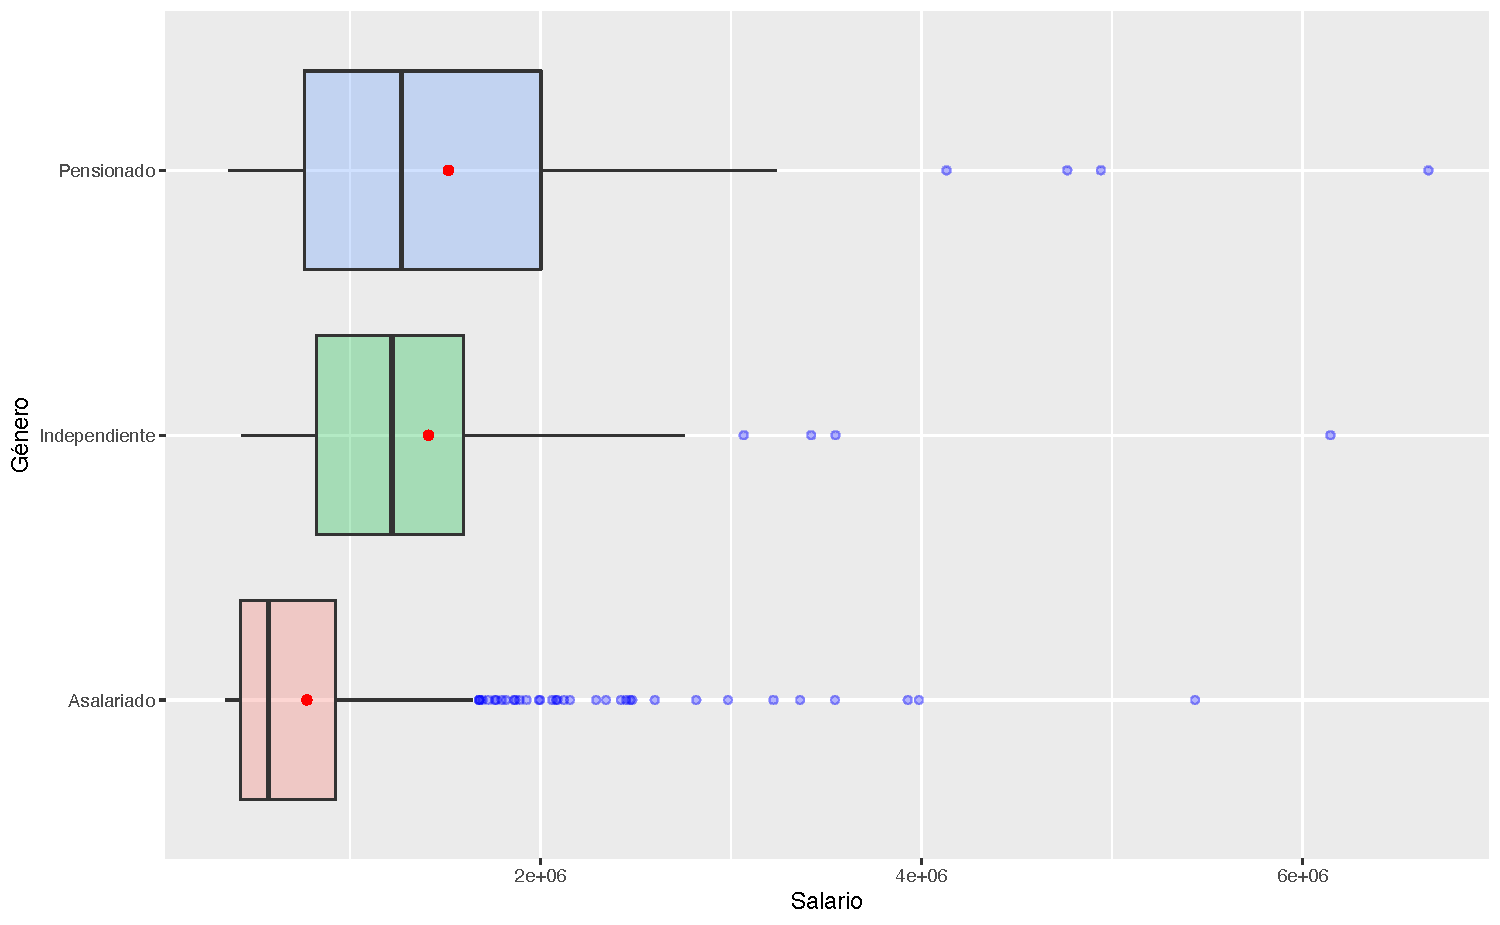
\includegraphics[width=1\linewidth]{Notas-Curso-Basico-R_files/figure-latex/notas-curso-154-1} \end{center}

\hypertarget{gruxe1ficos-de-barras}{%
\section{\texorpdfstring{\textbf{Gráficos de barras}}{Gráficos de barras}}\label{gruxe1ficos-de-barras}}

Los gráficos de barras, se utilizan comúnmente para representar variables categóricas (atributos u ordinales) y variables cuantitativas discretas.

\begin{Shaded}
\begin{Highlighting}[]
\FunctionTok{ggplot}\NormalTok{(datos.ingresos, }\FunctionTok{aes}\NormalTok{(tipo\_empleado)) }\SpecialCharTok{+}
  \FunctionTok{geom\_bar}\NormalTok{()}
\end{Highlighting}
\end{Shaded}

\begin{center}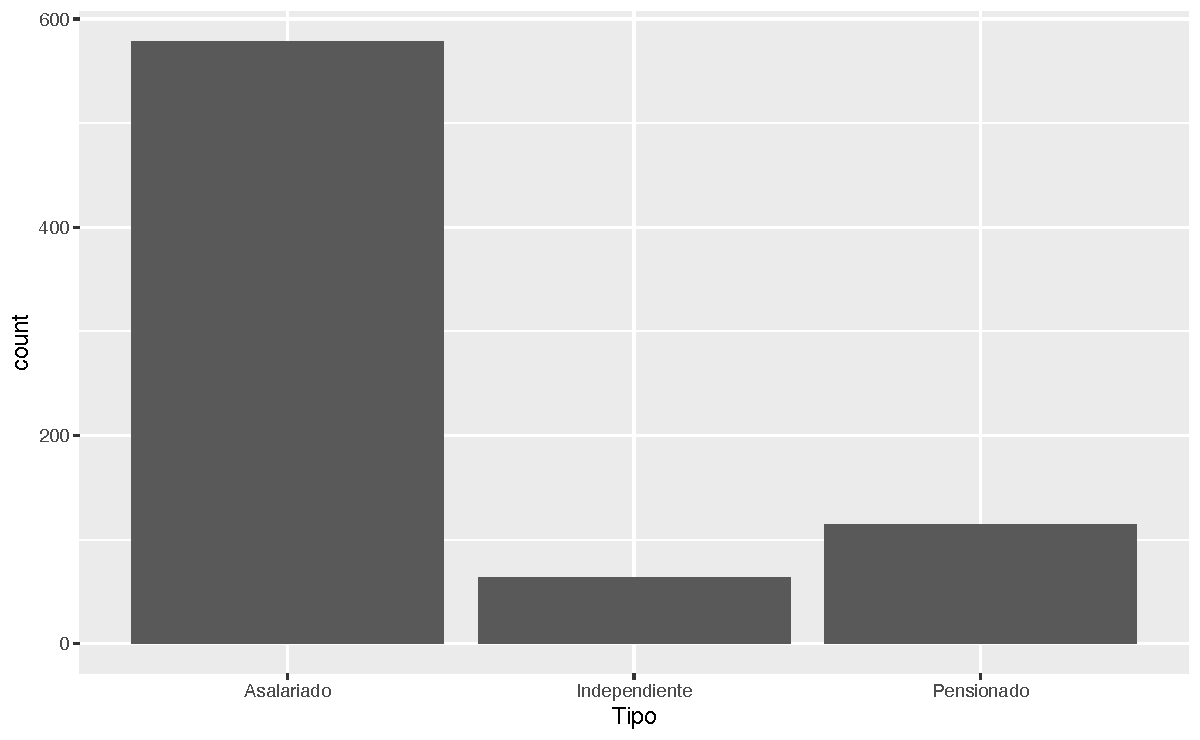
\includegraphics[width=1\linewidth]{Notas-Curso-Basico-R_files/figure-latex/notas-curso-155-1} \end{center}

\begin{Shaded}
\begin{Highlighting}[]
\FunctionTok{ggplot}\NormalTok{(datos.ingresos, }\FunctionTok{aes}\NormalTok{(tipo\_empleado)) }\SpecialCharTok{+}
  \FunctionTok{geom\_bar}\NormalTok{() }\SpecialCharTok{+}
  \FunctionTok{labs}\NormalTok{(}\AttributeTok{title =} \StringTok{"Gráfico de barras"}\NormalTok{,}
    \AttributeTok{x =} \StringTok{"Tipo cliente"}\NormalTok{,}
    \AttributeTok{y =} \StringTok{"Cantidad"}\NormalTok{)}
\end{Highlighting}
\end{Shaded}

\begin{center}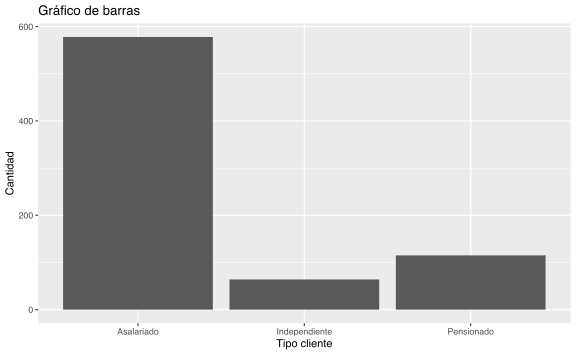
\includegraphics[width=1\linewidth]{Notas-Curso-Basico-R_files/figure-latex/notas-curso-156-1} \end{center}

\begin{Shaded}
\begin{Highlighting}[]
\FunctionTok{ggplot}\NormalTok{(datos.ingresos, }\FunctionTok{aes}\NormalTok{(tipo\_empleado, }\AttributeTok{fill =}\NormalTok{ sector\_empleo)) }\SpecialCharTok{+}
  \FunctionTok{geom\_bar}\NormalTok{() }\SpecialCharTok{+}
  \FunctionTok{labs}\NormalTok{(}\AttributeTok{title =} \StringTok{"Gráfico de barras"}\NormalTok{,}
    \AttributeTok{x =} \StringTok{"Tipo cliente"}\NormalTok{,}
    \AttributeTok{y =} \StringTok{"Cantidad"}\NormalTok{)}
\end{Highlighting}
\end{Shaded}

\begin{center}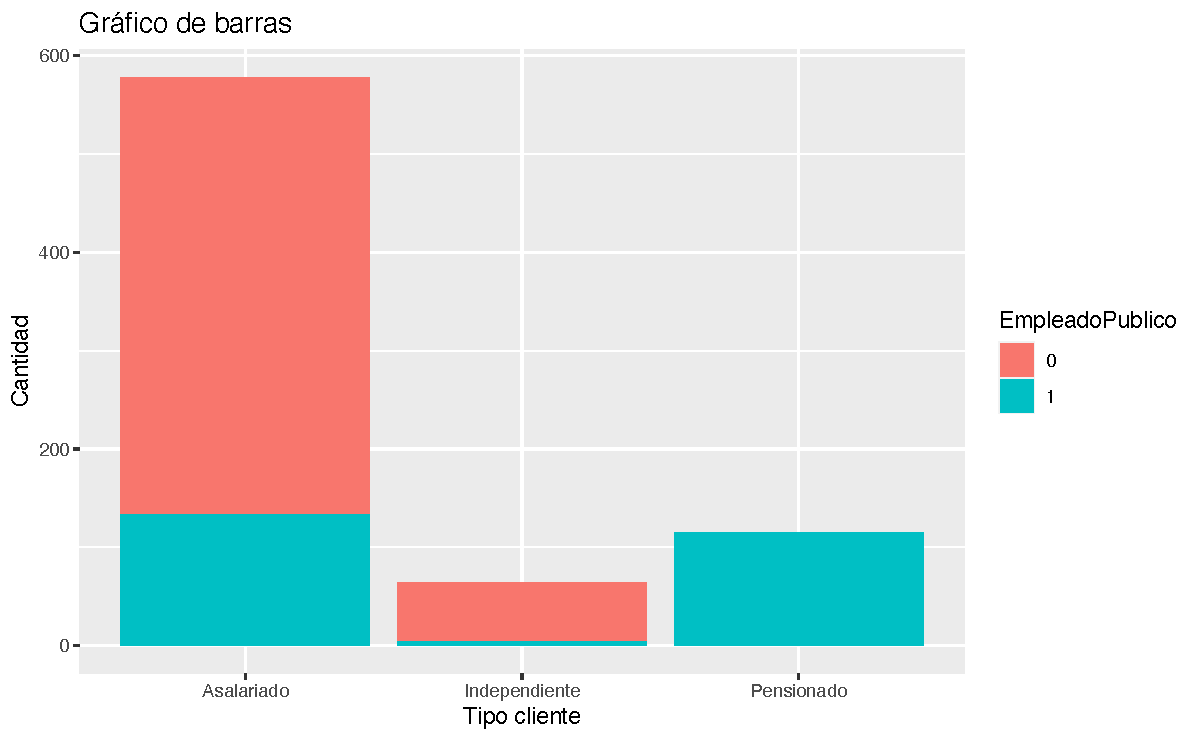
\includegraphics[width=1\linewidth]{Notas-Curso-Basico-R_files/figure-latex/notas-curso-157-1} \end{center}

\begin{Shaded}
\begin{Highlighting}[]
\FunctionTok{ggplot}\NormalTok{(datos.ingresos, }\FunctionTok{aes}\NormalTok{(}\AttributeTok{x =}\NormalTok{ tipo\_empleado, }\AttributeTok{fill =}\NormalTok{ sector\_empleo))  }\SpecialCharTok{+}
  \FunctionTok{geom\_bar}\NormalTok{() }\SpecialCharTok{+}
  \FunctionTok{labs}\NormalTok{(}\AttributeTok{x =} \StringTok{"Tipo cliente"}\NormalTok{, }\AttributeTok{y =} \StringTok{"Cantidad"}\NormalTok{) }\SpecialCharTok{+}
  \FunctionTok{scale\_x\_discrete}\NormalTok{(}\AttributeTok{labels =} \FunctionTok{c}\NormalTok{(}\StringTok{"Asalariado"}\NormalTok{, }\StringTok{"Independiente"}\NormalTok{, }\StringTok{"Pensionado"}\NormalTok{)) }\SpecialCharTok{+}
  \FunctionTok{scale\_fill\_discrete}\NormalTok{(}\StringTok{"Tipo empleado"}\NormalTok{,}
    \AttributeTok{labels =} \FunctionTok{c}\NormalTok{(}\StringTok{"Público"}\NormalTok{, }\StringTok{"Privado"}\NormalTok{))}
\end{Highlighting}
\end{Shaded}

\begin{center}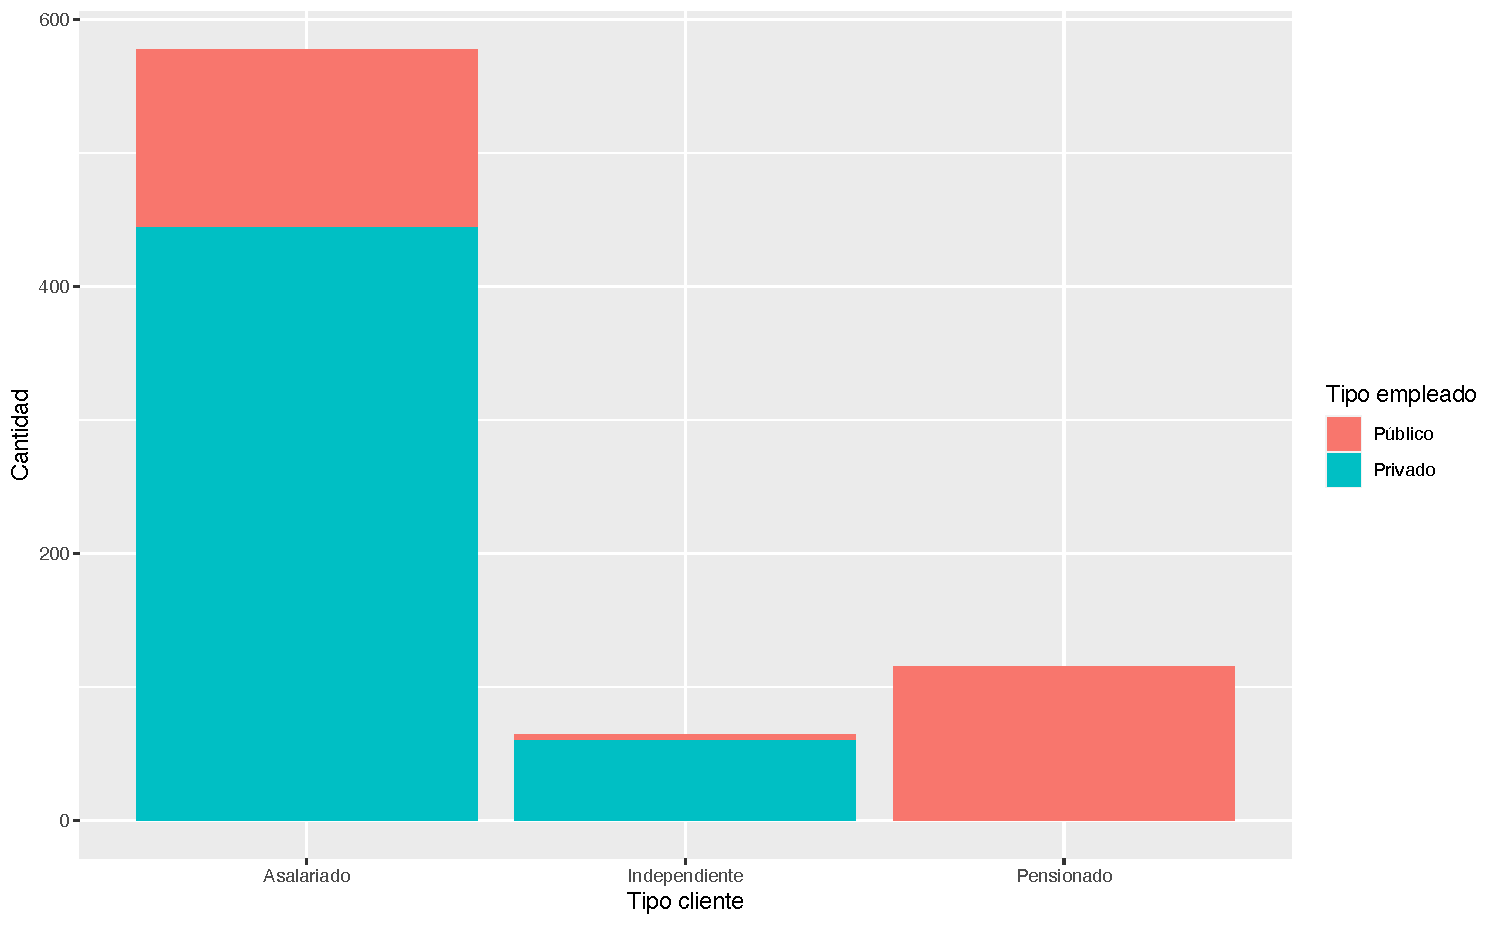
\includegraphics[width=1\linewidth]{Notas-Curso-Basico-R_files/figure-latex/notas-curso-158-1} \end{center}

\begin{Shaded}
\begin{Highlighting}[]
\FunctionTok{ggplot}\NormalTok{(datos.ingresos, }\FunctionTok{aes}\NormalTok{(}\AttributeTok{x =}\NormalTok{ tipo\_empleado, }\AttributeTok{fill =}\NormalTok{ sector\_empleo))  }\SpecialCharTok{+}
  \FunctionTok{geom\_bar}\NormalTok{() }\SpecialCharTok{+}
  \FunctionTok{labs}\NormalTok{(}\AttributeTok{x =} \StringTok{"Tipo cliente"}\NormalTok{, }\AttributeTok{y =} \StringTok{"Cantidad"}\NormalTok{) }\SpecialCharTok{+}
  \FunctionTok{scale\_x\_discrete}\NormalTok{(}\AttributeTok{labels =} \FunctionTok{c}\NormalTok{(}\StringTok{"Asalariado"}\NormalTok{, }\StringTok{"Independiente"}\NormalTok{, }\StringTok{"Pensionado"}\NormalTok{)) }\SpecialCharTok{+}
  \FunctionTok{scale\_fill\_discrete}\NormalTok{(}\StringTok{"Tipo empleado"}\NormalTok{,}
    \AttributeTok{labels =} \FunctionTok{c}\NormalTok{(}\StringTok{"Público"}\NormalTok{, }\StringTok{"Privado"}\NormalTok{)) }\SpecialCharTok{+}
  \FunctionTok{geom\_text}\NormalTok{(}\AttributeTok{stat =} \StringTok{"count"}\NormalTok{, }\FunctionTok{aes}\NormalTok{(}\AttributeTok{label =}\NormalTok{ ..count..),}
    \AttributeTok{position =} \StringTok{"stack"}\NormalTok{,}
    \AttributeTok{vjust =} \DecValTok{1}\NormalTok{,}
    \AttributeTok{size =} \DecValTok{2}\NormalTok{,}
    \AttributeTok{color =} \StringTok{"black"}\NormalTok{)}
\end{Highlighting}
\end{Shaded}

\begin{center}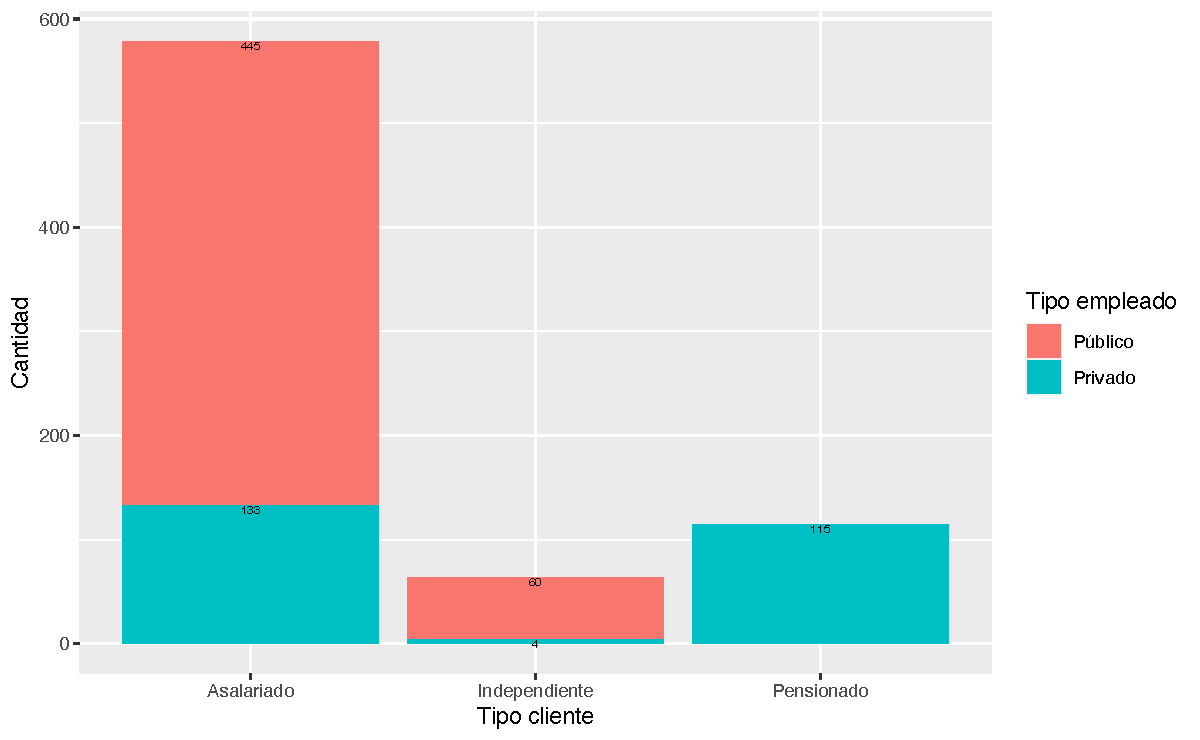
\includegraphics[width=1\linewidth]{Notas-Curso-Basico-R_files/figure-latex/notas-curso-159-1} \end{center}

\begin{Shaded}
\begin{Highlighting}[]
\FunctionTok{ggplot}\NormalTok{(datos.ingresos, }\FunctionTok{aes}\NormalTok{(}\AttributeTok{x =}\NormalTok{ tipo\_empleado, }\AttributeTok{fill =}\NormalTok{ sector\_empleo))  }\SpecialCharTok{+}
  \FunctionTok{geom\_bar}\NormalTok{() }\SpecialCharTok{+}
  \FunctionTok{labs}\NormalTok{(}\AttributeTok{x =} \StringTok{"Tipo cliente"}\NormalTok{, }\AttributeTok{y =} \StringTok{"Cantidad"}\NormalTok{) }\SpecialCharTok{+}
  \FunctionTok{scale\_x\_discrete}\NormalTok{(}\AttributeTok{labels =} \FunctionTok{c}\NormalTok{(}\StringTok{"Asalariado"}\NormalTok{, }\StringTok{"Independiente"}\NormalTok{, }\StringTok{"Pensionado"}\NormalTok{)) }\SpecialCharTok{+}
  \FunctionTok{scale\_fill\_discrete}\NormalTok{(}\StringTok{"Tipo empleado"}\NormalTok{,}
    \AttributeTok{labels =} \FunctionTok{c}\NormalTok{(}\StringTok{"Público"}\NormalTok{, }\StringTok{"Privado"}\NormalTok{)) }\SpecialCharTok{+}
  \FunctionTok{geom\_text}\NormalTok{(}\AttributeTok{stat =} \StringTok{"count"}\NormalTok{,}
    \FunctionTok{aes}\NormalTok{(}\AttributeTok{label =} \FunctionTok{paste}\NormalTok{(}\FunctionTok{round}\NormalTok{((..count..) }\SpecialCharTok{/} \FunctionTok{sum}\NormalTok{(..count..) }\SpecialCharTok{*} \DecValTok{100}\NormalTok{), }\StringTok{"\%"}\NormalTok{)),}
    \AttributeTok{position =} \StringTok{"stack"}\NormalTok{,}
    \AttributeTok{vjust =} \DecValTok{1}\NormalTok{,}
    \AttributeTok{size =} \DecValTok{2}\NormalTok{,}
    \AttributeTok{color =} \StringTok{"black"}\NormalTok{)}
\end{Highlighting}
\end{Shaded}

\begin{center}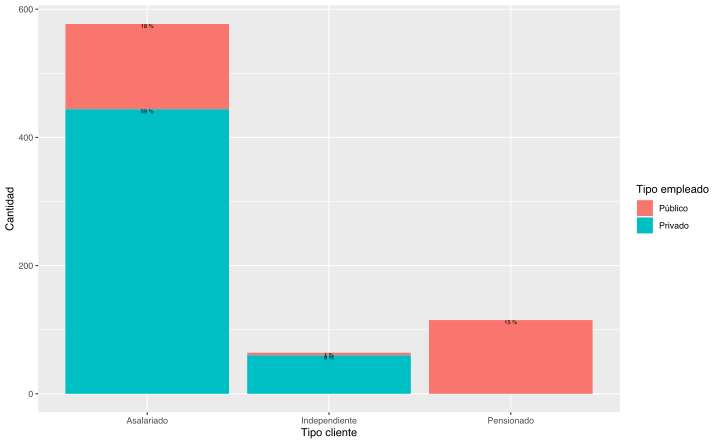
\includegraphics[width=1\linewidth]{Notas-Curso-Basico-R_files/figure-latex/notas-curso-160-1} \end{center}

\begin{Shaded}
\begin{Highlighting}[]
\FunctionTok{ggplot}\NormalTok{(datos.ingresos, }\FunctionTok{aes}\NormalTok{(}\AttributeTok{x =}\NormalTok{ tipo\_empleado, }\AttributeTok{fill =}\NormalTok{ sector\_empleo))  }\SpecialCharTok{+}
  \FunctionTok{geom\_bar}\NormalTok{(}\AttributeTok{position =} \StringTok{"fill"}\NormalTok{) }\SpecialCharTok{+}
  \FunctionTok{labs}\NormalTok{(}\AttributeTok{x =} \StringTok{"Tipo cliente"}\NormalTok{, }\AttributeTok{y =} \StringTok{"Cantidad"}\NormalTok{) }\SpecialCharTok{+}
  \FunctionTok{scale\_x\_discrete}\NormalTok{(}\AttributeTok{labels =} \FunctionTok{c}\NormalTok{(}\StringTok{"Asalariado"}\NormalTok{, }\StringTok{"Independiente"}\NormalTok{, }\StringTok{"Pensionado"}\NormalTok{)) }\SpecialCharTok{+}
  \FunctionTok{scale\_fill\_discrete}\NormalTok{(}\StringTok{"Tipo empleado"}\NormalTok{,}
    \AttributeTok{labels =} \FunctionTok{c}\NormalTok{(}\StringTok{"Público"}\NormalTok{, }\StringTok{"Privado"}\NormalTok{))}
\end{Highlighting}
\end{Shaded}

\begin{center}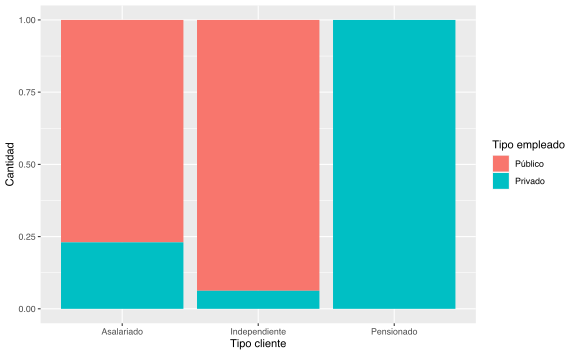
\includegraphics[width=1\linewidth]{Notas-Curso-Basico-R_files/figure-latex/notas-curso-161-1} \end{center}

\begin{Shaded}
\begin{Highlighting}[]
\FunctionTok{ggplot}\NormalTok{(datos.ingresos, }\FunctionTok{aes}\NormalTok{(}\AttributeTok{x =}\NormalTok{ tipo\_empleado, }\AttributeTok{fill =}\NormalTok{ sector\_empleo))  }\SpecialCharTok{+}
  \FunctionTok{geom\_bar}\NormalTok{(}\AttributeTok{position =} \StringTok{"dodge"}\NormalTok{) }\SpecialCharTok{+}
  \FunctionTok{labs}\NormalTok{(}\AttributeTok{x =} \StringTok{"Tipo cliente"}\NormalTok{, }\AttributeTok{y =} \StringTok{"Cantidad"}\NormalTok{) }\SpecialCharTok{+}
  \FunctionTok{scale\_x\_discrete}\NormalTok{(}\AttributeTok{labels =} \FunctionTok{c}\NormalTok{(}\StringTok{"Asalariado"}\NormalTok{, }\StringTok{"Independiente"}\NormalTok{, }\StringTok{"Pensionado"}\NormalTok{)) }\SpecialCharTok{+}
  \FunctionTok{scale\_fill\_discrete}\NormalTok{(}\StringTok{"Tipo empleado"}\NormalTok{,}
    \AttributeTok{labels =} \FunctionTok{c}\NormalTok{(}\StringTok{"Público"}\NormalTok{, }\StringTok{"Privado"}\NormalTok{))}
\end{Highlighting}
\end{Shaded}

\begin{center}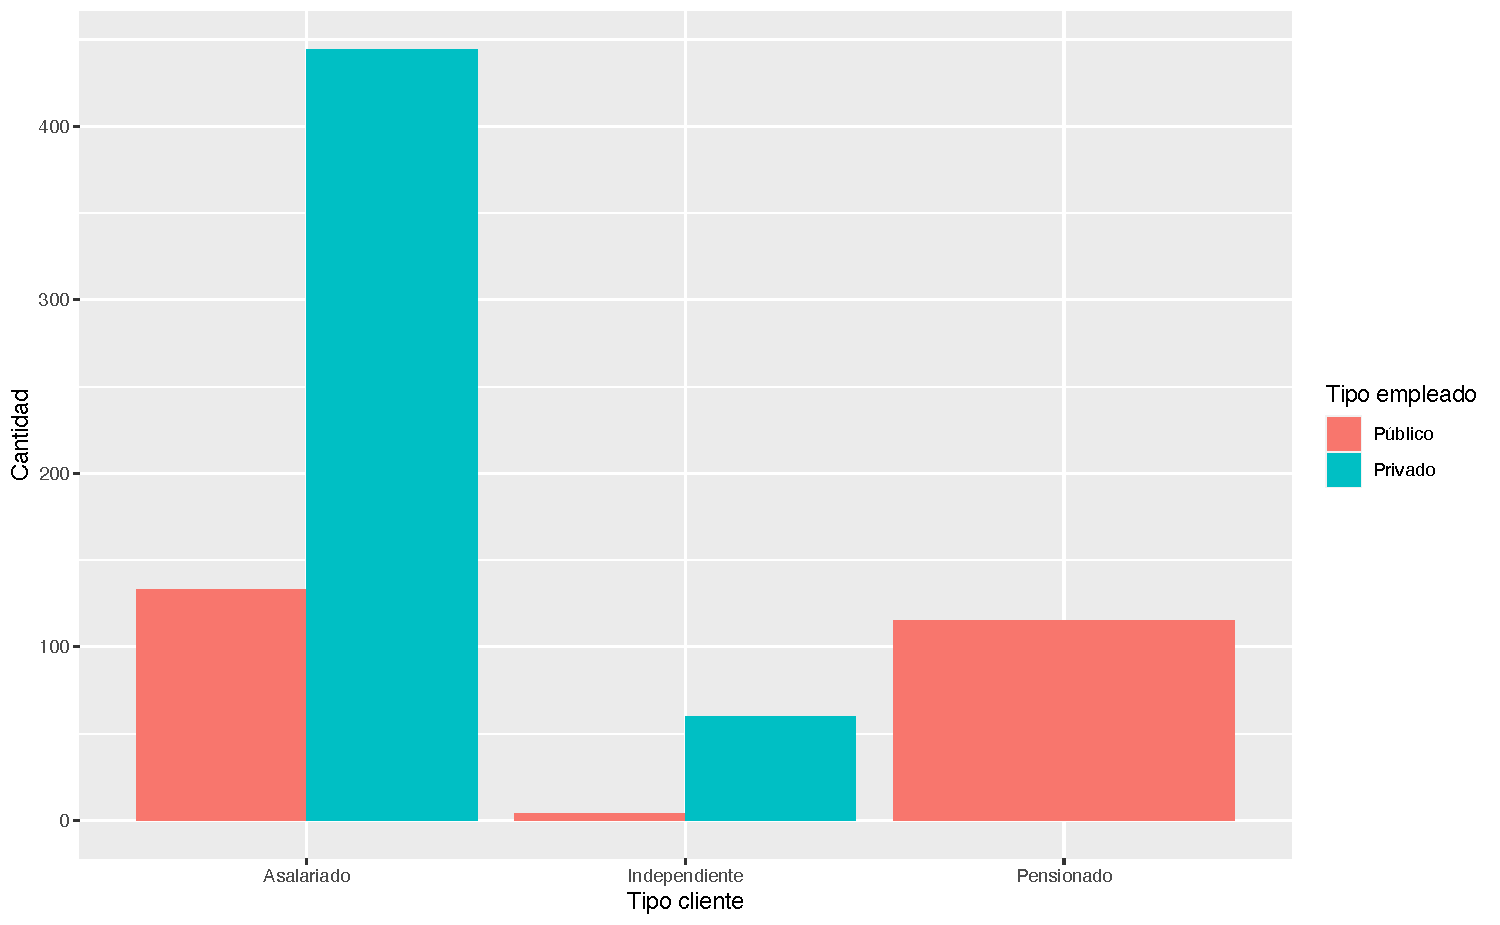
\includegraphics[width=1\linewidth]{Notas-Curso-Basico-R_files/figure-latex/notas-curso-162-1} \end{center}

\end{document}
